% XeTeX-Header zur Definition des Dokuments
% XeTeX-Vorlage für Abschlußarbeiten an der Universität Bielefeld
% ---------------------------------------------------------------------
% Stand, 07. Juni 2010
%
% Timo Reuter (treuter@cit-ec.uni-bielefeld.de), AG Semantic Computing
% Exzellenzcluster für Cognitive Interaction Technology
%
% Dies Vorlage setzt die Schriftart FagoNo sowie einen XeTeX-Kompiler 
% voraus. Alle Dokumente müssen zwingend mit Unicode (UTF-8) als
% Kodierung abgespeichert werden.

\documentclass[
  a4paper,              % Wir verwenden A4 Papier
  %oneside,             % Einseitiger Druck
  twoside,              % Zweiseitiger Druck
  12pt,                 % Große Schrift, besser geeignet für A4
  halfparskip,          % Halbe Zeile Abstand zwischen Absätzen
  chapterprefix,        % Kapitel mit 'Kapitel' anschreiben
  headsepline,          % Linie nach Kopfzeile
  footsepline,          % Linie vor Fußzeile
  bibtotocnumbered,     % Literaturverzeichnis im Inhaltsverzeichnis numeriert einfügen
  DIV=15,
  BCOR=8mm
]{scrbook}

% Kopf-/ und Fußzeilen
\usepackage{footmisc}

% Parts haben im Inhaltsverzeichnis keine Seitenzahlen
\makeatletter
\let\partbackup\l@part
\renewcommand*\l@part[2]{\partbackup{#1}{}}
\makeatother

% Zeichencodierung des Dokuments und des Zeichensatzes.
\usepackage{pifont}
\usepackage{fontspec}
\usepackage{xunicode}
\usepackage{xltxtra}
\usepackage{textcomp}
\usepackage{csquotes}

% Lokalisierung auf deutsch (Silbentrennung usw.)
%\usepackage[german]{babel}
\usepackage[english]{babel}

% Paket um Grafiken im Dokument einbetten zu können.
\usepackage{graphicx}
\graphicspath{{images/}}

% PDF-Merkmale
\usepackage[
  pdftitle={Memory-based exploratory online learning of simple object manipulation},            % Titel des PDF Dokuments.
  pdfauthor={Jan Pöppel},                 % Autor des PDF Dokuments.
  pdfsubject={Memory-based exploratory online learning of simple object manipulation},          % Thema des PDF Dokuments.
  pdfcreator={Texlive, XeTeX},           % Erzeuger des PDF Dokuments.
  pdfkeywords={Keyword1, keyword2},      % Schlüsselwörter für das PDF.
  pdfpagemode=UseOutlines,               % Inhaltsverzeichnis anzeigen beim Öffnen
  bookmarksopen=false,                   % Inhaltsverzeichnisbaum geöffnet anzeigen
  pdfdisplaydoctitle=true,               % Dokumenttitel statt Dateiname anzeigen.
  pdflang=en                             % Sprache des Dokuments.
]{hyperref}

% Schriften
\defaultfontfeatures{Mapping=tex-text}
\setmainfont[ItalicFont={FagoNo}, BoldFont={FagoNoLf-Bold}]{Latin Modern Roman} %{GoudyOlSt BT}
\setsansfont{FagoNo}
%{\setmonofont{Arial}\fontsize{48pt}{\baselineskip}\selectfont}
%\usepackage{default}

% Farben definieren
\usepackage{color, colortbl}
\definecolor{LinkColor}{rgb}{0,0,0}
\definecolor{ListingBackground}{rgb}{0.85,0.85,0.85}
\definecolor{LightGrey}{rgb}{0.93,0.93,0.93}
\definecolor{LightGrey2}{rgb}{0.9,0.9,0.9}
\definecolor{DarkGrey}{rgb}{0.65,0.65,0.65}
\definecolor{UniBiGreen}{rgb}{0.0,0.457,0.336}
\definecolor{CitecOrange}{rgb}{0.93,0.453,0.004}

% Farbeinstellungen für die Verweise im PDF-Dokument.
\hypersetup{
  colorlinks=true,       % Aktivieren von farbigen Verweisen im Dokument (ohne Rahmen)
  linkcolor=LinkColor,   % Farbe festlegen.
  citecolor=LinkColor,   % Farbe festlegen.
  filecolor=LinkColor,   % Farbe festlegen.
  menucolor=LinkColor,   % Farbe festlegen.
  urlcolor=LinkColor,    % Farbe von URL's im Dokument.
  bookmarksnumbered=true % Überschriftsnummerierung im PDF Inhalt anzeigen.
}

% Beschriftungen für Bilder und Tabellen
\setcapindent{1em} % Zeilenumbruch bei Bildbeschreibungen.
\setkomafont{captionlabel}{\fontspec[Color=656565, Scale=0.7]{FagoNoLf-Bold}} % Beschriftungen für Bilder und Tabellen
\setkomafont{caption}{\fontspec[Color=656565, Scale=0.7]{FagoNoLf-Bold}} % Beschriftungen für Bilder und Tabellen
\setkomafont{descriptionlabel}{\fontspec{FagoNoLf-Bold}} % Optionales Label in der description-Umgebung


% Stil der Kopf- und Fußzeilen
\usepackage[footsepline,plainfootsepline]{scrpage2}
\pagestyle{scrheadings}
\setheadsepline{}[\color{DarkGrey}]    % Kopfzeilenlinie
\setfootsepline{}[\color{DarkGrey}]    % Fußzeilenlinie
\renewcommand*{\partpagestyle}{empty}  % Parts haben keine Kopf-/Fußzeile

% Überschriften
\setkomafont{sectioning}{\normalfont\bfseries} % Titel mit Normalschrift
\addtokomafont{sectioning}{\fontspec{FagoNoLf-Bold}}
\addtokomafont{pagehead}{\fontspec[Color=656565]{FagoNoLf-Bold}}   % Seitentitel
\addtokomafont{pagenumber}{\fontspec[Color=656565]{FagoNoLf-Bold}} % Fußnoten

% Stil der Überschriften
\usepackage[Lenny]{sty/fncychapleo}

% Paket um Quelltext sauber zu formatieren.
%\usepackage[savemem]{listings}
%% Einstellungen für das 'listings' Paket.
%\lstloadlanguages{C}            % Sprache laden, notwendig wegen Option 'savemem'
%\lstset{
%	language=C,                 % Sprache des Quelltexts ist C
%	numbers=left,               % Zelennummern links
%	stepnumber=1,               % Jede Zeile numerieren.
%	numbersep=5pt,              % 5pt Abstand zum Quellcode
%	numberstyle=\tiny,          % Zeichengröße 'tiny' für die Nummern.
%	breaklines=true,            % Zeilen umbrechen, wenn notwendig.
%	breakautoindent=true,       % Nach dem Zeilenumbruch Zeile einrücken.
%	postbreak=\space,           % Bei Leerzeichen umbrechen.
%	tabsize=2,                  % Tabulatorgröße (Indent) ist 2
%	basicstyle=\ttfamily\scriptsize, % Schrift
%	showspaces=false,           % Leerzeichen nicht anzeigen.
%	showstringspaces=false,     % Leerzeichen auch in Zeichenketten ('') nicht anzeigen.
%	extendedchars=true,         % Alle Zeichen vom Latin1 Zeichensatz anzeigen.
%	backgroundcolor=\color{ListingBackground}, % Hintergrundfarbe des Quelltexts setzen.
%	captionpos=b,               % Caption unten
%    %linewidth=0.9\textwidth,   % base line width
%    xleftmargin=0.02\textwidth, % margin left
%    xrightmargin=0.02\textwidth % margin right
%}


\usepackage[linesnumbered]{algorithm2e}
\SetAlFnt{\ttfamily\small}

\usepackage{amsmath}
%\DeclareMathOperator*{\argmin}{arg\,min}
\newcommand{\argmin}{\operatornamewithlimits{argmin}}

\usepackage[e]{esvect}
\makeatletter
\def\traitfill@#1#2#3#4{%
  $\m@th\mkern2mu\relax#4#1\mkern-6.0mu%
   \cleaders\hbox{$#4\mkern0mu#2\mkern0mu$}\hfill%
   \mkern-1.5mu#3$%
}
 \makeatother
\renewcommand{\vec}[1]{\vv{#1}}

% Tabellen
\usepackage{array}                  % Paket für erweiterte Tabelleneigenschaften
\usepackage{multirow}               % Zusammengefaßte Reihen in Tabellen ermöglichen
\setlength{\arrayrulewidth}{0.7pt}
\setlength{\extrarowheight}{3pt}
\arrayrulecolor{DarkGrey}           
\usepackage{longtable}              % Ermöglicht sich über mehrere Seiten erstreckende Tabellen
\usepackage{tabularx}               % Mächtigere Tabellenumgebung


% Stil für Designboxen
\newcommand{\designbox}[2]{
  \hspace*{17pt}
  \begin{tabular*}{402pt}{p{378pt}p{0pt}}
    \begin{flushright}\fontspec[Color=656565, Scale=0.9]{FagoNoLf-Bold}#1\hspace*{-18.5pt}\vspace*{-16pt}\end{flushright}\\
    \hline
    \cellcolor{LightGrey}\fontspec{FagoNo}#2 & \cellcolor{DarkGrey}\\
    \begin{picture}(0,0)
      \put(245,13){\color{DarkGrey}\rule{151pt}{0.5pt}}
    \end{picture}
  \end{tabular*}
}

% Bibliographie-Stil
%\usepackage{apacite}         % Psychologie
\usepackage[numbers]{natbib}  % Linguistik und Naturwissenschaften

% Silbentrennung für Wörter, die nicht vom Babel-Paket erkannt werden
\hyphenation{Dezi-mal-trenn-zeichen In-stal-la-ti-ons-as-sis-tent}

%Abkürzungen
%\usepackage{acronym}

%Glossary and Acronyms

\usepackage[nomain,toc,acronyms]{glossaries}
%\chapter{Acronyms}
%\begin{acronym}[Bash]
% \acro{ITM}{Instantaneous Topological Map}
% \acro{GNG}{Growing Neural Gas}
% \acro{LLM}{Local Linear Map}
%\end{acronym}

\newacronym{itm}{ITM}{Instantaneous Topological Map}
\newacronym{aitm}{AITM}{Adapted Instantaneous Topological Map}
\newacronym{gng}{GNG}{Growing Neural Gas}
\newacronym{llm}{LLM}{Local Linear Map}
\newacronym{nn}{NN}{Nearest Neighbour}
\newacronym{knn}{\textit{k}-NN}{k-Nearest Neighbour}
\newacronym{rnn}{RNN}{recurrent neural network}
\newacronym{bn}{BN}{Bayesian Network}
\makeglossaries
% Überschriften anpassen
%\usepackage{titlesec}
%\titleformat{\subsection}{\bfseries\large\sffamily\itshape}{}{0em}{\thesubsection~}
% Folgende Dinge tut man in TeX NICHT, da das Ganze gegen die Grundregeln des
% Textsatzes verstößt. Wer meint, es trotzdem verwenden zu müssen, um ein "Word"-ähnlicheres 
% Satzbild zu bekommen, sollte mit dem Verantwortlichen über Sinn oder Unsinn dieses 
% Vorhabens diskutieren und diese "Hacks" möglichst unterlassen.

% Zeilenabstand ändern (Standard bei TeX ist 1,2)
%\usepackage{setspace}
%\onehalfspacing % Ergibt 1,5 Zeilenabstand
%\doublespacing % Ergibt 2,0 Zeilenabstand

% Seitenränder ändern
%\usepackage{anysize}
%\marginsize{2.5cm}{2cm}{2.5cm}{2.5cm}




\begin{document}
  % Römische Nummerierung für Einleitung mit Index usw.
  \pagenumbering{roman}

  % Titelseite definieren
\begin{titlepage}

  % Alles zentriert darstellen
  \begin{center}

    \setlength{\unitlength}{1mm}
    
    % Graphische Elemente auf der Seite platzieren
    \begin{picture}(0,0)
      \put(-55,5){\color{CitecOrange}\rule{15cm}{5mm}}
      \put(-105,-10){\color{CitecOrange}\rule{20cm}{1.52cm}}
      \put(-105,-15){\color{CitecOrange}\rule{18cm}{5.2mm}}
      
      \put(-40,-8){\fontspec[Color=fefefe, Scale=3.6]{FagoNoLf-Bold}Master Thesis}

      %\put(-90,12){\color{UniBiGreen}\rule{12mm}{12mm}}
     % \put(-84,10){\color{UniBiGreen}\rule{29mm}{10mm}}      
     % \put(-82.5,12){\fontspec[Color=fefefe, Scale=0.66]{FagoNoLf-Bold}Universität Bielefeld}
      
      \put(-90,-230){\color{CitecOrange}\rule{20cm}{2.5mm}}
    \end{picture}

    \vspace{3cm} % Vertikaler Abstand von 25pt

    % Name der Universität, der Fakultät und (optional) des Studiengangs
    {\fontspec[Color=101010, Scale=2.0]{FagoNoLf-Bold}Bielefeld University} \\
    \vspace{10pt} % Vertikaler Abstand von 10pt
    {\fontspec[Color=101010, Scale=1.7]{FagoNo}Faculty of Technology }
    %\vspace{10pt} % Vertikaler Abstand von 10pt
    %{\huge Studiengang ISY}

    \vspace{35pt} % Vertikaler Abstand von 35pt

    % Titel der Arbeit
    {\fontspec[Color=101010, Scale=2.5]{FagoNoLf-Bold} Memory-based exploratory online learning of simple object manipulation} \\
    \vspace{10pt} % Vertikaler Abstand von 10pt
    %{\fontspec[Color=101010, Scale=2.5]{FagoNoLf-Bold} \textbf{einen schönen Titel hat}} \\
    %\vspace{10pt} % Vertikaler Abstand von 10pt

    \vspace{40pt} % Vertikaler Abstand von 40pt

    % Angestrebter Abschluß wird hier eingetragen (B.Sc./M.Sc./B.A./etc.)
    {\fontspec[Color=101010, Scale=1.0]{FagoNo}In Partial Fulfillment of the Requirements for the Degree of} \\
    \vspace{5pt}
    {\fontspec[Color=101010, Scale=1.5]{FagoNoLf-Bold}Master of Science (M.Sc.)}

    \vspace{40pt} % Vertikaler Abstand von 40pt

    % Name des Students/der Studenten
    {\fontspec[Color=101010, Scale=1.5]{FagoNo}Jan Pöppel} \\
    \vspace{5pt} % Vertikaler Abstand von 5pt
  
    % Monat und Jahr der Arbeit (Abgabedatum)
    {\fontspec[Color=101010, Scale=1.2]{FagoNo}September 2015}

    \vspace{50pt} % Vertikaler Abstand von 40pt

  \end{center}

    {
      \begin{tabular}{ll}
        \vspace{5pt} % Vertikaler Abstand von 5pt
        \fontspec[Color=101010, Scale=1.0]{FagoNo}Referee:  & \fontspec[Color=101010, Scale=1.0]{FagoNo}Apl. Prof. Dr.-Ing. Stefan Kopp \\
        \vspace{5pt} % Vertikaler Abstand von 5pt
        \fontspec[Color=101010, Scale=1.0]{FagoNo}Referee: & \fontspec[Color=101010, Scale=1.0]{FagoNo}Dipl.-Inf. Maximilian Panzner \\
      \end{tabular}
    }
    


\end{titlepage}
  % Abstract

% Der Abstract wird nicht ins Inhaltsverzeichnis aufgenommen

%\chapter*{\enskip Abstract}

%Dies ist eine gute Zusammenfassung, warum der Leser diesen Text lesen sollte.

% Übersetzte Version
\chapter*{\enskip Abstract}

The classical machine learning approach is to train suitable models on reasonable big data sets before deployment. However, this approach is not suitable in many scenarios such as robotics due to scarcity of data. Furthermore, general purpose robots are expected to be able to deal with unknown circumstances. This requires the ability to incrementally adapt to unknown situations.

This thesis considers learning about simply object manipulations such as pushing as a simplified scenario of adapting to unknown environments.
Within this context, this thesis suggests and discusses two memory-based concepts that challenge the tasks of incremental online learning with limited domain knowledge.
The concepts learn forward and inverse models of their environment, allowing them to predict future states as well as incrementally reach desired target states.

The learned forward and inverse models of the environment's dynamics are evaluated separately in different scenarios.
The evaluations show that the proposed methods both successfully learn to predict future states and interact with their given environment while providing insight of remaining problems.


 % Abstract
  %% Widmung/Zitat/Motto der Arbeit

\cleardoublepage

  ~
  \vspace{370pt} % Vertikaler Abstand von 370pt

  \begin{tabularx}{0.9\textwidth}{Xl}
      & {\large »Hier könnte eine} \\
      & {\large Widmung für jemanden} \\
      & {\large stehen«} \\
  \end{tabularx}

  \vspace{0pt}

  \begin{tabularx}{0.9\textwidth}{Xr}
      & \textit{Zitierter Autor}\\
  \end{tabularx}

\cleardoublepage
 % Widmung/Zitat
  
  \tableofcontents  % Inhaltsverzeichnis
%  \listoffigures    % Bildverzeichnis
%  \listoftables     % Tabellenverzeichnis

  \cleardoublepage  % Seitennummerierung neustarten

  % Arabische Nummerierung für den Hauptteil
  \pagenumbering{arabic}
  
  % Einzelne Kapitel werden hier eingefügt
  \chapter{Introduction}

%Motivate necessity
%State goals
%Structure of thesis
%What is the problem that we try to solve?
%Why is it relevant to solve it?


%TODO delete? Most likely not good...
%The defining quality that any agent, artificial or natural, requires is learning. Also used for many different 
%phenomenons, the term learning at its core means adaptation. The agent or some part of it adapts in order to
%better deal with its environment. Natural agents, especially humans, display impressive learning capabilities,
%allowing them to quickly adapt to ever changing environments and new tasks.
%
%In recent years, machine learning has come a long way in understanding and reproducing some of the learning
%capabilities of humans. We now have a wide range of different techniques and algorithms that can yield good
%classification and regression results. %TODO make glossary to explain what classification and regression is
%In introduction to these can for example be found in book by Bishop \cite{bishop}.
%
%The quality of the results achieved by machine learning is however more dependent on the chosen representation
%of the problem then on the actual technique used. For example it is generally not sufficient to use the raw audio signals 
%for speech recognition \cite{speechRecog}. Instead most speech recognizers use carefully selected pre-computed
%features that allow the underlying machine learner to correctly distinguish the words. 
%
%Because finding the best features is as challenging as learning a problem itself, a lot of focus as recently 
%shifted to deep learning \cite{deepLearning}. Deep learning is a technique that is inspired by the human brain and refers to
%training neural networks with many thousands of artificial neurons. Properly trained, these networks are capable of finding 
%relevant features in the presented data by themselves \cite{deepLearningFeatures}. Currently the biggest
%problem with deep learning is the required amount of training before the network can be used successfully. Although recent
%advances such as the development of Hinton's dropout technique \cite{dropout} allows to train bigger networks with fewer data,
%this criteria still limits the potential use cases of deep learning and neural networks in general.

After decades of research a vast amount of powerful tools have been developed for machine learning. A good overview can be found in the book by Bishop \cite{bishop}. Each of these methods has its own advantages and disadvantages and are applicable to certain situations. Currently, research in machine learning is often performed by choosing a problem, e.g. image recognition or movement control, and trying to find and tune the most successful method to solve the chosen problem. This way the researchers were able to create better classifiers for image recognition (e.g. \cite{imageRecList}) and better controllers for complex movements (e.g.\cite{movementList}).
%TODO Adrianas Anmerkung: 1. Im ersten Absatz würde ich das "e.g. image recognition or movement
%control" weglassen. Das kommt direkt im nächsten Satz schon wieder
%(und image recognition im 3. Absatz noch einmal), das stört dann etwas
%den Lesefluss, wenn man so denkt "häh, déjà vu?!"


In most of these cases the machine is trained to solve one specific problem. Depending on the chosen methods it is not possible to extend the machines knowledge easily without retraining the entire system afterwards because of the stability-plasticity-problem \cite{stability-plasticity}. More precisely because of the phenomenon of catastrophic forgetting \cite{catastrophicForgetting1}.

With advances in robotic hardware and the successful application of machine learning in specialized tasks, such as image recognition, the goal of robotic research trends towards multi-purpose robots. However, the biggest problem for multi-purpose machines is that the current approach to machine learning is not applicable. Since the number of tasks the robot has to face is not known in advance, suitable tools cannot be training in advance. Furthermore, even if one would attempt to train specialized parts for all kinds of problems, acquiring sufficient and accurate training data beforehand is infeasible at best. 
%TODO glossary for model or some footnode on what is meant by model
Therefore, instead of trying to train the machine beforehand, it might be better to provide it with the means to adapt to new situations on its own while it is encountering them. Instead of learning on previously recorded training data, the robot adapts its model to the continuous stream of data while it is already using what it learned beforehand. The biggest reason against such an continuous incremental approach is its difficulty. When incrementally training a single model to solve multiple different problems, the catastrophic forgetting effect is usually experienced. The usual approach is learn local models for each task separately, however this introduces the need to recognize and distinguish the different problems in order to know which kind of local model the robot needs to employ. 

Instead of challenging the entire problem of incrementally learning an unlimited number of arbitrary tasks, this thesis concentrates on the incremental learning of one task without prior training. 
While there are multiple machine learning methods that allow incremental updates, not all of them are suitable for this kind of task. First of all, the method should be as independent on prior knowledge as possible so that it can be used for a wide variety of task the robot might encounter. Furthermore, the update and query times of the chosen method need to be quick enough to allow continuous interaction with the environment. On top of that, the chosen method should not suffer from the catastrophic forgetting effect since the robot would constantly keep updating it. For this thesis a memory based learning approach was chosen in order to solve these problems. Due to their one-shot learning ability, memory based methods can produce good prediction results from very little training data. 

One important aspect of general purpose robotics is object manipulation. In order to successfully interact with the objects in its environment the robot needs to learn what kind of interactions are possible and what their effects are. 
Furthermore, object interactions are hard to model manually as they follow complex dynamics. On top of that, different object can behave completely differently, so that knowledge acquired in previous training sessions might not be useful later on. It is for these reasons object interactions make an ideal target for online self adaptation. 

This thesis provides two concepts that provide incremental learning of pushing interactions between an actuator controlled by action primitives and some object in the environment.
While pushing interactions are only a very small subset of possible interactions a robot can have with objects, their dynamics still provide sufficient complexity to evaluate incremental learning systems. Since the behavior of differently shaped objects can vary a lot, learning about different kind of objects can even be regarded as learning similar but different tasks.%TODO Maybe more on this?
The proposed concepts need to provide a forward model as well as an inverse model. The forward model makes predictions about the state of all entities in the environment after an action primitives as been performed. The inverse model provides an action primitive that is used to reach a specified target configuration within the environment.

The goal of this thesis can summarized to provide and evaluate simple models that:
%TODO planning and lifelong are mentioned here for the first time and not explained!!!
\begin{enumerate}
	\item Update themselves incrementally during the interaction
	\item Allow prediction and planning of simple object interactions % with minimal domain knowledge
	\item Allow lifelong learning
\end{enumerate}

This thesis is structured as follows: In chapter \ref{chap:stateOfTheArt} an overview over memory based learning as well as recently proposed models for learning object interactions for robotics is given. Two concepts were developed in order to fulfill the stated goals. Their general idea is described in \ref{chap:concept} before concrete implementation details are given in chapter \ref{chap:modelReal}. These models are then evaluated with regards to their prediction and planning performance in chapter \ref{chap:evaluation}. Finally, this thesis concludes with a discussion of these results in chapter \ref{chap:conclusion}.


  \chapter{Related Work \label{chap:stateOfTheArt}}


%What kinds of interaction models are there
%Incremental/online models
%Memory based approaches
%What have others tried to solve this/similar problems?
%TODO get authors automatically

%TODO mention at least one paper where a pairwise interaction representation is used!
\section{Memory based models}

In machine learning, one generally assumes that data, for example class labels, are given by some function $f^*$. Given some training data $D$ with $d^i =(\vec{x}^i,\vec{y}^i)$ where $\vec{x}^i$ represents the given input and $\vec{y}^i$ the corresponding output of the $i$'s data point, one tries to estimate $f^*$. 
Although different algorithms approximate $f^*$ differently, they can be categorized in two general families: The first one tries to detect \textit{correlations} between features in order to make predictions. The simplest example for this is given by the linear regression \cite{linearRegression} where they find weights $w_j$ so that $f(\vec{x}) = \sum w_j \cdot x_j$. 

The other family focuses more on \textit{similarities} in the input space instead of feature correlations. Maybe the most prominent example for this is the \gls{knn} regression \cite{knn}. Previously seen training data is stored and compared to new input data. New input data $\vec{x}$ is then labeled according to the $k$ closest stored instances. The easiest form is to average the outputs of the $k$ closest instances around $\vec{x}$ (here denoted as the set $N(\vec{x}$)):
\begin{equation}
\vec{y}(\vec{x}) = \frac{1}{k} \sum_{\vec{y} \in N(\vec{x})} \vec{y}
\end{equation} %TODO double y, change?

These instances are also often called prototypes, if only a few instances are used to represent a subspace in the input space. Since the closest instance is determined by similarity, the used features and metric is usually critical for these methods \cite{importanceOfMetric/Features}. This dependence on careful preprocessing of the used features and metric can be considered the biggest disadvantage of these methods. However, there has also been a lot of research in automatically adapting the used metric while training in order to better fit the data, e.g. by Hammer et al. \cite{lvq}. Unfortunately, online metric adaptation often needs a lot of iterations before yielding satisfying results. 

Another disadvantage of memory based models is the memory consumption over time. Since the training examples need to be stored in order to be retrieved later, a lot of memory can be consumed. This can also lead to increased query and update times, since these scale linearly with the number of stored instances. Geva et al. \cite{protReduction} showed already 1991 that the number of required instances can be reduced depending on the used algorithm. Extending the area of influence of the given instances, for example by using \glspl{llm} \cite{LLM}, can further decrease the number of required instances.

The advantages of memory, or instance based models is that they are local by design. This means that their output only depends on a small part, located around the given input, of the model. Likewise, when they are updated by adding or removing some stored instances, they do so based on local criteria. This is also the reason that memory based models usually do not suffer from the catastrophic forgetting phenomenon.

For the implementation of the concepts developed in this thesis, an adaptation of the \gls{gng} using \gls{llm} as output function is used as underlying regression model. The \gls{aitm} is explained in section \ref{sec:ITM} in detail.

%TODO consider putting it in, when we actually talk about exploration
%\section{Learning forward and inverse models}
%
%Much research in the field of robotics has gone into learning forward and inverse models for robot control \cite{listOfControlPaper}. 
%
%
%\item \cite{baranes2013active} Robot architecture for active, online learning of forward and inverse models
%\begin{itemize}
%	\item Limited to only the robot, not including external objects and their interactions
%	\item Highlights some of the challenges when trying to (actively) learn online
%\end{itemize}

\section{Learning object interactions}

Because of the importance for robotics, a lot of research is being done regarding object interactions.  However, most systems are trained in an offline fashion \cite{nishide2008predicting, moldovan2012learning, contactPrediction}. Out of these, the works of Moldovan et al. and Kroemer et al. are most notable:
Moldovan et al. use a probabilistic approach to learn affordance models useful for object interactions in \cite{moldovan2012learning}. Affordances, as introduced by Gibson \cite{affordances}, describe the relations between object, actions and effects. Moldovan et al. are able to extend their approach to multiple object scenarios. The biggest difference of their approach to the here presented one, apart from the required offline training and tuning, is that it uses more prior knowledge in order to construct a suitable \gls{bn}.

More recently, Kroemer et al. developed a memory based model that uses the similarities between contact distributions between objects in order to classify different kind of interactions in \cite{contactPrediction}. In their work an interaction is for example if one object supports another object or if an object can be lifted given a certain grasp configuration. The approach of Kroemer et al. also works with multiple objects since only the contact distributions between two objects were considered. Unfortunately, their approach is limited to binary predictions of predefined interaction classes. The robot still needs to learn a suitable forward model. Furthermore, their proposed sampling approach showed poor performance and is likely to become infeasible in unconstrained complex environments.

Learning object interaction incrementally has also been done:
In \cite{levine2015learning} Levine et al. achieved great results in learning policies of complex dynamics %TODO \gls{policy}.
such as assembling plastic toys. They require much fewer training iterations than earlier policy search approaches, i.e in \cite{otherPolicySearchs}. They achieve this by training linear-Gaussian controllers on trajectories which are later combined by a guided policy search component.
However, the main difference to the given problem for this thesis is that Levine et al. consider the objects already firmly grasped which eliminates most of the dynamics in the interaction between the grasped object and the actuator.

The most similar work to this thesis both in terms of setting and in their approach has been done by 
Lau et al. in \cite{pushing}. The authors use \gls{knn} regression to make predictions about pushing an object. They also provide an algorithm to extract suitable actions that allow to push the object towards a specified target. Unfortunately, the authors restrict their model to the pushing interaction: Moving the actuator, here the entire circular mobile robot, around or towards the object is not part of the learned model but provided instead. Furthermore, while they describe their approach to work with position and orientation, they only provide results for position. 
%Although, developed from a different point of view, the work presented here can be considered an extension to their work. Especially the proposed alternative inverse model (see section \ref{sec:invModel}) 

%\begin{itemize}
%	\item \cite{pushing} Paper using similar idea of instance based memory in order to predict pushing
%	\begin{itemize}
%		\item restricted to only pushing interactions (no getting closer etc learned by model)
%		\item is mainly used to move object to target position
%		\item General strategy is the same as in my model: First figure out preconditions, then perform best action
%		\item Uses nearest neighbor to find best action
%		\item Works for complex shaped objects
%		\item Paper only shows results based on position, not orientation
%		
%	\end{itemize}
%	\item \cite{nishide2008predicting} RNN and HNN system that learns interactions between objects from camera images
%	\begin{itemize}
%		\item Tries to solve more complex problem (includes feature extraction from images in the system)
%		\item But is learned in a batch mode. Prerecorded by controlling the robot and training on recorded images (~ 20min offline)
%		\item They call it \textit{active sensing} regardless
%	\end{itemize}
%	\item \cite{baranes2013active} Robot architecture for active, online learning of forward and inverse models
%	\begin{itemize}
%		\item Limited to only the robot, not including external objects and their interactions
%		\item Highlights some of the challenges when trying to (actively) learn online
%	\end{itemize}
%	\item \cite{flanagan2006control} Recent (2006) paper about human object manipulation control strategies
%	\item \cite{moldovan2012learning} Learning object affordances with probabilistic model. Actually extends to multiple objects
%	\item \cite{levine2015learning} Impressive (batch) results of object manipulation.
%	\begin{itemize}
%		\item Restriction is that objects are fixed to robot
%		\item Basically \textit{only} learns a trajectory
%	\end{itemize}
%	\item \cite{contactPrediction} Exemplar-based learning of contact/support interaction between (multiple) objects.
%	\begin{itemize}
%		\item Contact distributions are estimated from contact points extracted from the point clouds of objects
%		\item Similarity between distributions determines whether the given contact allows a special interaction
%		\item Binary classification if a certain interaction is possible/happening
%		\item Does not make predictions about the future state of the interacted objects
%		\item Has not been trained online, but rather with previously labeled training data
%	\end{itemize}
%	\begin{itemize}
%		\item Look at experience graphs
%		\item Can be mentioned here as well (\cite{phillips2012graphs}) as somewhat similar idea regarding the use of previous experiences, maybe better in introduction?
%	\end{itemize}
%\end{itemize}

  \chapter{Concept \label{chap:concept}}

%Big picture
%General ideas how to solve goals
%Present equal concepts with theoretical pro's and cons
%What are the general ideas that we try to solve the problem with?

%TODO check possible acronyms: nearest neighbor, abstract collection!!
%TODO make sure to write things like abstract collection the same every time (ie abstract collection vs Abstract Collection) !!

Instead of using only a single regression model that is constantly updated and queried, the robot needs some sort of architecture in order to deal with the continuous information stream. This architecture needs to organize the incoming data and determine what should be learned from these experiences. Furthermore, the architecture can combine different components in order to make the best use of what it has learned. 
This chapter presents the two concepts that were developed in order to fulfill these tasks. These two concepts differentiate mainly in the way they represent the interactions that they learn about. The first concept, further described in section \ref{sec:pairInt}, uses pairwise interactions to represent the objects in the environment. In the alternative approach, described in section \ref{sec:gate}, the objects are represented individually. Additionally, a gating function is introduced to distinguish when one object actually influences another. 
A special inverse model is proposed in section \ref{sec:invModel} that is tailored to the continuous interaction with the environment. %TODO more either here or in the introduction?
Before going into the description of both concepts and the inverse model, section \ref{sec:problem} summarizes the actual problem these concepts need to solve. 

%Unlike in isolated classification or regression tasks, it is not enough to employ one specialized machine learning algorithm in order to solve the given problem. Since the model is supposed to interact with its environment and update itself while experiencing new interactions, a more important complex model is required. While the chosen underlying regression and classification methods need to fulfill certain conditions and greatly influence the resulting model performance, they could easily replaced by suitable alternatives. Even more important is the architecture around them, that organizes the information coming from the environment and adapts where necessary. This chapter presents the general concepts behind the two developed models and the way the information is organized.
%
%First a more detailed specification about the problem is given in section \ref{sec:problem}. Afterwards,
%section \ref{sec:pairInt} describes the first developed concepts working solely in what is called the interaction space in this thesis. The alternative approach of modeling object states directly is described in section \ref{sec:gate}.

\section{Problem specification \label{sec:problem}}

As stated in the introduction, the goal of this thesis is to provide possible models that incrementally learn simple pushing interactions between physical objects. 
More specifically, the model needs to learn two tasks:

1) Given some known action primitive that controls the robots actuator, the models need to learn to predict the next states of all objects in the environment (\textit{forward model}). 
While these action primitives are determined beforehand, the model does not necessarily know the effects of the primitives. In this case, the model needs to not only learn about the pushing interactions, but also about the consequences of its own actions.

2) The robot is supposed to be able to reach some specified target configuration (\textit{inverse model}). Any object in the environment, not just the actuator, can be specified which means that the model must learn how it can influence the objects through its actuator. The target configurations will rarely be reachable within a single action primitive but the inverse model should provide actions that reduce the distance to the target configuration. 
Since the actuator can only influence another object by pushing it, the actuator might be required to circle around an object in order to be able to move it towards the desired configuration.

A sequence of action primitives that would reach the target after their execution is not requested. This is because the models are expected to react to changes in the environment directly. Furthermore, if such a sequence is required, for example in order to make higher level plans, they can be created using the two features provided these two tasks.

Both of these tasks need to be learned incrementally without prior training. This requires the model to be tightly coupled to the environment. An overview about the models interaction with the environment can be seen in figure \ref{fig:overview}. The model is updated each time feedback from the environment is received, allowing better predictions.

\begin{figure}
	\centering
	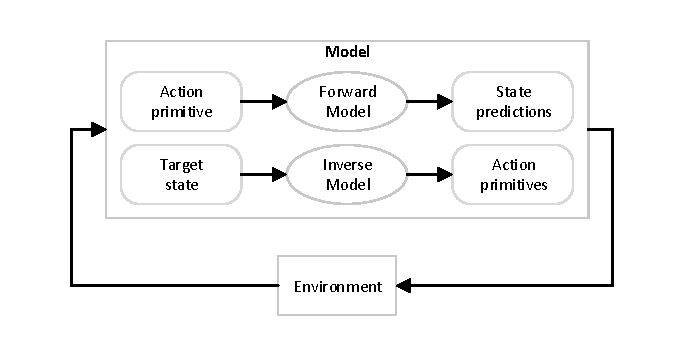
\includegraphics{Overview.pdf}
	\caption{Overview of the problem. The model includes a forward model in order to make predictions given the current environment state and a certain action primitive. When given a target state the inverse model provides suitable action primitives to reach the desired state.}
	\label{fig:overview}
\end{figure}

\section{Modeling pairwise interactions \label{sec:pairInt}}
%TODO rework, don't quite like this yet...
The first approach tries to find distinct subspaces in the \textit{interaction space} between two objects. In this context, the pairwise interaction space represents the space of all interactions between two objects. This includes their relative placement and movement to each other, as well as their influence, for example by pushing, on each other. Instead of modeling and learning forward and inverse models for each object separately, only the pairwise interaction space between two objects is considered. %TODO this kind of already determins differential/local features. Check how those are introduced later! 

For every object pair an \textit{interaction state} is considered. This interaction state represents one object's state relative to the other object's state. This includes for example transforming each objects position and orientation to the local coordinate system of the reference object. %For the realization, described in section \ref{sec:pairRealization}, he actuator is not used as reference.
The predicted object states are extracted from the predicted interaction states. The way these interaction states are computed from the object states and how the object states can be extracted from the predicted interaction states, need to be provided to the model beforehand. %TODO elaborate more on this?

At each update step the current interaction states for all object pairs are computed from the information provided by the environment. The previous state, the performed action and the resulting state are collected and stored as an \textit{episode} $e$. The general idea is to store these episodes as past knowledge, similar to the approach in case based reasoning \cite{cbr}. When predicting, these episodes can be searched for the most similar one. The similarity can be determined by comparing the previous state of each episode to the given interaction state and the used action to the current action:

\begin{equation}
e^{best} = \argmin_{e^i \in E} ||e^i_{preState}-curState, e^i_{action}-curAction||_{ep}
\label{eq:bestEpisode}
\end{equation}


$e^i$ represents the i's episode that has been stored yet. $e^i_{preState}$ means only the previous interaction state of the episode, while $e^i_{action}$ represents the used action in that episode.
The norm $||a,b||_{ep}$ is used to allow different weighting of the features from the previous state and the action. For planning, the action difference can be replaced by the difference between the resulting state of each episode and the desired target state.

Once the most similar episode has been found, the desired information can be extracted from it. For prediction, this corresponds to the resulting state in the episode, whereas it corresponds to the action for the inverse case. The formula above represents a nearest neighbor search on all episodes. Although such an approach can work, it quickly becomes infeasible when the number of stored episode keeps growing. Since the nearest neighbor search scales linearly with the number of stored examples it is unsuitable for lifelong learning. %TODO lifelong not introduced...
Furthermore, the simple nearest neighbor approach does not offer good generalization since it does not interpolate between similar episodes. 

As mentioned at the beginning of this chapter, the idea of this concept is to split the interaction space into subspaces and train local models for each of these subspaces. An overview of the proposed architecture can be seen in figure \ref{fig:PairOverview}.
All episodes corresponding to the same subspace are collected in \textit{Abstract Collections}. Each collection can train its own local forward and inverse model which is explained in section \ref{sec:ACs}.
An \textit{Abstract Collection Selector} is needed in order to choose the most appropriate abstract collection in a given situation. 

%The realization of this concept is described in section \ref{sec:pairRealization}.

\begin{figure}
	\centering
	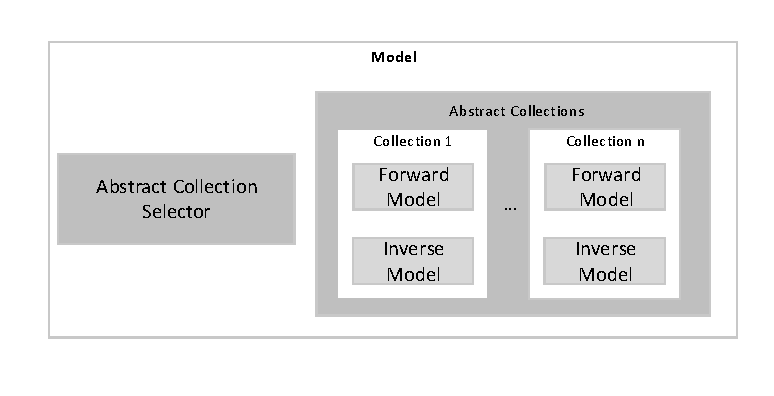
\includegraphics{PairwiseOverview.pdf}
	\caption{Overview of the model in interaction space. The different abstract collections contain forward and inverse models of distinct subspaces of the interaction space. The selector is needed in order to select the correct submodel for prediction.}%TODO consider adding transformation to interaction state and back to object states as well?} %TODO
	\label{fig:PairOverview}
\end{figure}

\subsection{Abstract Collection \label{sec:ACs}}

The interaction space can be split in a multitude of subspaces. Ideally, one would want to split the space in subspaces with some semantic meaning, for example into \textit{no interaction}, \textit{turning} and \textit{pushing}. In this example, the no interaction subspace would correspond to the episodes where the actuator moves without influencing another object. Turning would correspond to an interaction where mainly the orientation of an object changes through the interaction. Lastly, the position of an object changes mainly in the pushing subspace. However, in order to separate the episodes like that, accurate labels are required. Such a classification is infeasible without prior domain knowledge. 
Instead of relying on domain knowledge, this approach uses the information available to the robot from the environment: The changing features within an episode.

In order to split the interaction space into subspaces, episodes that correspond to the same local group are clustered together.
The clustering of episodes suggested here is based on the set of features that changed between the previous state and the resulting state while performing an action. The set $S$ of features that changed is defined as follows 
\begin{equation}
S = \{f | f \in F ~ \wedge ~ ||Pre(f)-Post(f)|| > \epsilon_{Noise}\}
\label{eq:difSet}
\end{equation}
where $F$ denotes the set of all features. $Pre(f)$ and $Post(f)$ denote the value of 
feature $f$ in the initial and resulting state of the episode respectively. $\epsilon_{Noise}$ is a threshold to cancel out potential noise of the environment and should be set according to the accuracy of the used sensors. Ideally, one would like to have feature specific thresholds since the possible range of the features might vary. However, this would require the model to have additional information about each feature.

Each different set is represented by its own \gls{ac}. The 
idea is that, while not necessarily holding semantic meaning directly, these collections correspond to different interaction scenarios. Depending on the features used, some \glspl{ac} might even be interpreted semantically.
Consider an exemplary interaction state with two features. The first feature represents the closest distance between the two objects in the interaction state. The second feature represents the angular direction of the second object with respect to the local coordinate system of the reference object. While the model itself has no knowledge about what each feature represents, a maximum of four \glspl{ac} can be created: No feature changes, either one of the two features changes and both change at the same time. In this example the \gls{ac} containing only the distance feature represents all interactions where one object moves straight towards or away from the other object. The set where nothing changes would signal a pushing interaction, considering a movement action was performed. While not all created \glspl{ac} can be interpreted semantically, the model can create these separations without any knowledge about what is represented by the features.

Since each distinct interaction scenario results in a different set of changing features, the interaction space is split into subspaces by these collections. The resulting collections create an abstract representation for each of these interaction scenarios. 

These collections can train their respective local forward and inverse models based on the episodes associated with them. Any suitable regression method can be used for these local models. The above mentioned nearest neighbor structure that works directly on the recorded episodes is just one simple example. Since the collections are independent of each other, different collections can even use different methods if desired. Furthermore, local optimizations such as feature selection could be performed in each collection. %TODO mention feature selection when it is not done/evaluated currently?

\subsection{Object state prediction with the Abstract Collection Selector \label{sec:pairPrediction}}

Prediction within this architecture requires several steps. The general idea of the information flow when predicting one interaction state is visualized in figure \ref{fig:PairPrediction}. The model expects an interaction state that has been computed from the objects information provided by the environment. This interaction state is used together with the given action primitive as input for the Abstract Collection Selector. The selector needs to estimate which \gls{ac} is most likely responsible for the next interaction. In order to make this estimation, any suitable classifier, e.g. a decision tree \cite{decisionTree}, is trained on all input-collection pairs the model experienced so far. 
%TODO maybe remove/rewrite this following passage
The total number of collections is limited to the size of the superset of $F$, although in practice, not all possibilities are likely. Furthermore, collections with less than $\epsilon_{min}$ training examples can be ignored. This threshold is used to reduce the number of outliers when training the classifier. %TODO this threshold does not exist anymore in the current implementation!!

After the most likely \gls{ac} has been selected, its forward model can be consulted for the prediction. The local model is queried using the interaction state together with the given action primitive as input. The output of the local model is the predicted interaction state. 
More precisely, the local model predicts how the current interaction state changes. These predicted changes are then added to features of the given interaction state this \gls{ac} is responsible for.
The predictions of the actual object states need to be extracted from this interaction state. The extraction depends on the actual features used and needs to be provided to the user just like the structure of the interaction state itself.

\begin{figure}
	\centering
	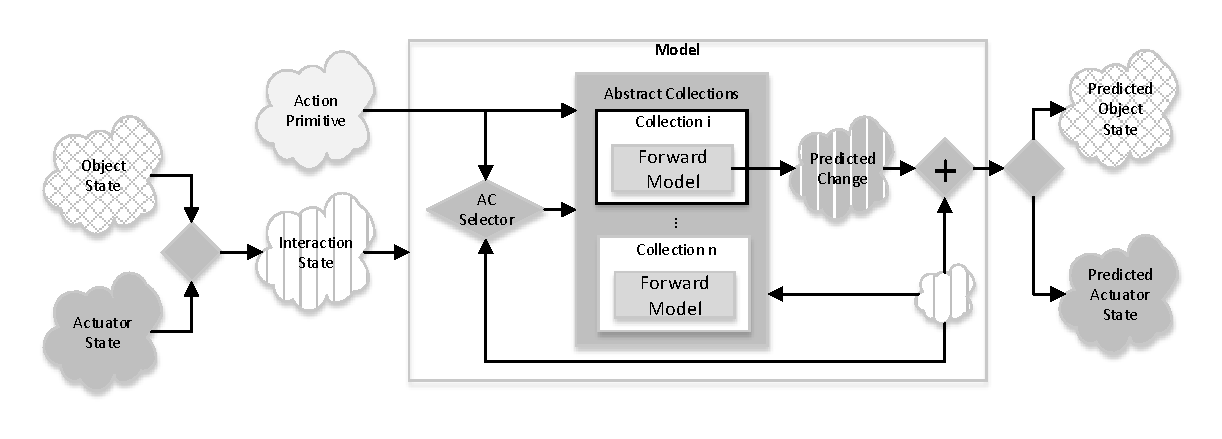
\includegraphics[width=\textwidth]{PairwisePrediction2.pdf}
	\caption{Concept of prediction in the pairwise interaction space with Abstract Collections. First the interaction state is computed. This state is then fed to the model together with the chosen action primitive. The AC Selector uses those to select the responsible Abstract Collection. The collection then uses its forward model to predict the changes in the interaction state. These changes are added to the given interaction state in order to compute the resulting prediction. The actual predicted object states are finally extracted from this interaction state.} 
	\label{fig:PairPrediction}
\end{figure}

\subsection{From target state to action primitive \label{sec:pairPlanning}}

%TODO
%(TODO consider redoing the planning algorithm more similar to the way it is done
%in the most recent model, which works, maybe the same ideas can be employed 
%here)

In order to get a suitable action primitive given a target configuration several steps are required as visualized in figure \ref{fig:PairPlanning}. 
First the difference state between the current situation and the target configuration is computed. Similar to the computation within the episodes above, a difference set $S$ can be computed from this difference state. Afterwards, the \gls{ac} that corresponds to the same set of features is selected. In the case that this collection is not yet known, the most similar collection is chosen instead. In this context, the most similar \gls{ac} is the one that covers most of the changed features in the computed difference set. If multiple alternatives exist, the \gls{ac} responsible for the changes in the most features is chosen. This is because more changing features means that the inverse model has more degrees of freedom to reach the target.

The selected \gls{ac} queries its own inverse model for preconditions that produce a change in the direction of the desired target configuration. 
Since it might not be possible to move an object directly in the desired direction due to the current position of the actuator, simply returning the action primitive is not sufficient.

The preconditions need to be checked against the currently given configuration of the target object and the actuator. If these preconditions are mostly fulfilled an action primitive can be extracted, otherwise, an intermediate target needs to be determined. This intermediate target represents a configuration for the actuator where the preconditions are met.

\begin{figure}
	\centering
	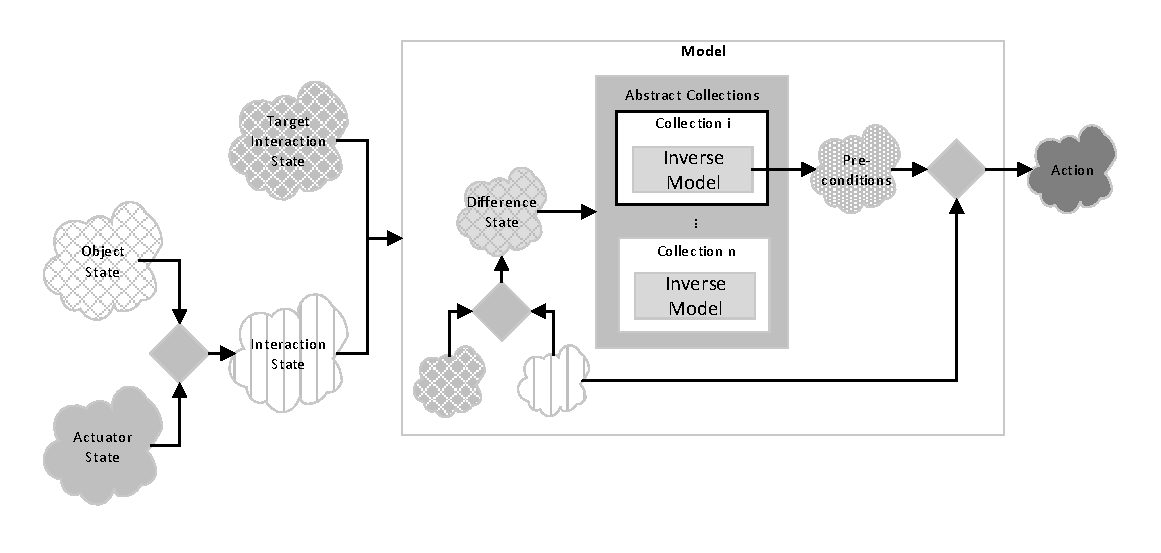
\includegraphics[width=\textwidth]{PairwisePlanning.pdf}
	\caption{Concept of computing suitable action primitives in order to reach a given target configuration. The suitable Abstract Collection is determined by the Difference State. An action primitive is computed from the preconditions returned by the inverse model.} 
	\label{fig:PairPlanning}
\end{figure}

%The action is then checked by consulting the already trained forward models. 
%In case the forward models predict that the selected action does not reduce the difference to the target, a different action needs to be selected. This is done by querying a different abstract collection. Alternatively, a random action can be performed in order to produce new episodes. These in turn would improve both the forward as well as the inverse models of their respective abstract collections.

\subsection{Theoretical discussion \label{sec:interactionTheory}}
%TODO do not really like this yet
The two core ideas of this concept are the use of a pairwise representation and splitting the interaction space. The splitting is done in order to allow the training of simpler local regression models. Furthermore, using local models avoids having to compare to all previously seen training examples. 
Using a global regression model, for example for the inverse model, is obviously possible as well, especially if the used model does not suffer from the complexity of the used interaction state and the continuous training. In this case, there is no need to determine the responsible \acrlong{ac}.

Using pairwise interaction states in order to represent the interactions between objects is often used in robotics, for example in \cite{pairwiseExamples}. 
Its advantage is that it represents both objects involved in an interaction at the same time. This means that only one regression model needs to be trained in order to make predictions about both objects. In theory this should also make it less likely that impossible configurations are predicted such as solid objects being inside of each other. Furthermore, such an interaction state can contain all the necessary information about the objects in one representation. 

The downside of this approach is that the actual object states need to be inferred from these interaction states. When using only differential features to construct the pairwise interaction state, this will only involve simple coordinate transformations. Some other object attributes might not be as easily transformable. Furthermore, in order to contain all the necessary information about both objects, these interaction states can become high dimensional. All computations from object to interaction states and vise versa need to be performed outside this proposed model.

Although the coupling of the two objects can have its advantages as stated above, the dependence between the objects can also be a problem when predicting. Any erroneous prediction will immediately affect two objects. 
Furthermore, when one of the two objects is represented relative to the coordinate frame of the other object, all predictions are also made with regard to the reference object's coordinate frame. 
In case the state of the reference object is not accurate, for example because of a sensor malfunction, the predictions for both objects will be influenced by this error. Imagine an error in the reference object's position. When using differential features, this error will directly be included in the prediction for both objects since the second object's position needs to be computed based on the inaccurate reference object's position.

An even bigger disadvantage is the fact that this approach cannot easily be extended to multiple objects. In environments with at least two objects and an actuator at least three pairwise interaction states are necessary: One for the first object and the actuator, one for the second object and the actuator and at least one for both objects. 
While one can argue for and against using the actuator as the reference object for the general case, depending on the actual scenario, this decision is not trivial between two objects. 
Even if one finds suitable reference objects, there is still a problem with the extraction of the actual object states after prediction. All objects are part of at least two interaction states in this scene. Therefore, at least two extracted predictions exist for all objects in the environment. Unfortunately, these predictions are likely to be different from another. It is therefore required to compute a final prediction for each object which is not trivial in the general case. Furthermore, the presented concept does not even know about object states, meaning that the final computation would need to be performed outside of the concept.
On top of that, the local models of the Abstract Collections need to be applicable to interaction states featuring different objects, making them more complicated.

%Regardless of the used representation, the proposed concept might have further issues:
Regarding the Abstract Collections:
Unfortunately, no guarantees can be given about how well the interaction space is split. Depending on the used features, as well as the actual interaction scenarios that are encountered, some abstract collections might cover most of the interaction space. 

%TODO Maybe this is rather discussion?
%Furthermore, if the Abstract Collection Selector, selects wrong collections it is still possible to predict impossible configurations. Just consider the situation where the actuator is in contact with an object but the Abstract Collection Selector selects a collection where only the actuator changes its position. In this case the actuator would be predicted to be inside the object, although no such interaction state has ever been seen.

\section{Object space with gating function \label{sec:gate}}

The alternative to modeling the interaction space, is to model each object and perform predictions for each object separately. 
The general components of this architecture are visualized in figure \ref{fig:GateOverview}.
The idea is to train local forward and inverse models for each object, or object group in the \textit{Predictor}. %TODO consider changing this name
Instead of distinguishing between different interaction scenarios as in the previous concept, objects that behave differently are distinguished. 
An object group can be considered a collection of objects that are similar in the way they behave during interactions. Therefore they can be represented by a single local model. One example would be two identically shaped block objects that only have different colors. In order to detect if two objects should be grouped together or not, one can start with training separate local models and compare their outputs. If two models appear to be similar, they can be merged together. Ideally, a similarity measure for objects is provided. Following the assumption that similar objects should behave similarly, such a measure would allow immediate grouping of objects.

Apart from the difference in representation, the other big difference in the two concepts is the introduction of the gating function (\textit{Gate} in the figure). The gating function is used to split the interaction space in two big subspaces. The first subspace represents all scenarios where no actual pushing interactions are taking place. That means that at most the actuator is moving due to some action primitives but no other object is influenced by those movements. Consequently, the other subspace contains all the scenarios where an object is influenced. When making predictions for the first subspace, it is sufficient to make predictions about the next state of the actuator. No knowledge about the behavior of the objects is required which also means that the local models do not need to be trained for these scenarios. The local object models only need to be trained on the scenarios where an object's state actually changes. 
This makes the local subspaces each model needs to learn already simpler then the interaction space learned in the previous concept. Therefore, multiple models for each object are not required.

In order to allow the local models to only train on this restricted subspace, this concept makes an additional assumption about the environment: 
This idea assumes that object states do not change without any interaction. The only exception is the \textit{Actuator}. Here, the actuator is treated as a special kind of object with its own forward and inverse model. These models can be provided beforehand or learned online.  

The current state of each object, including the actuator, is always updated when new information is received from the environment. At each update the gating function and if required the actuator's local models are trained. On top of that, the local models responsible for any object whose state changed with the last update, are trained as well.


\begin{figure}
	\centering
	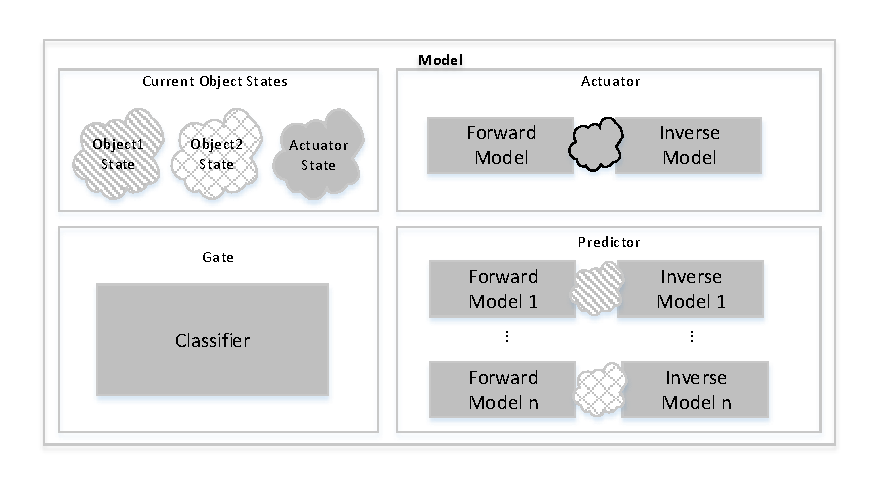
\includegraphics{GateOverview.pdf}
	\caption{Overview of the concept about object state with gate. The actuator is a special object, that can be influenced directly. It's forward and inverse model might even be provided if known. For the other objects/object groups, the Predictor learns these models. The Gate learns a classifier to distinguish interactions between objects from only single object changes.} 
	\label{fig:GateOverview}
\end{figure}

\subsection{Object state prediction \label{sec:gatePrediction}}

Because of the assumption that objects other than the actuator cannot change without any interaction, the way prediction is performed differs between the different object types. The actuator simply queries its own forward model with the selected action primitive in order to predict the next actuator state. 
The general process for predicting the next state of other objects is visualized in figure \ref{fig:GatePrediction}.

\begin{figure}
	\centering
	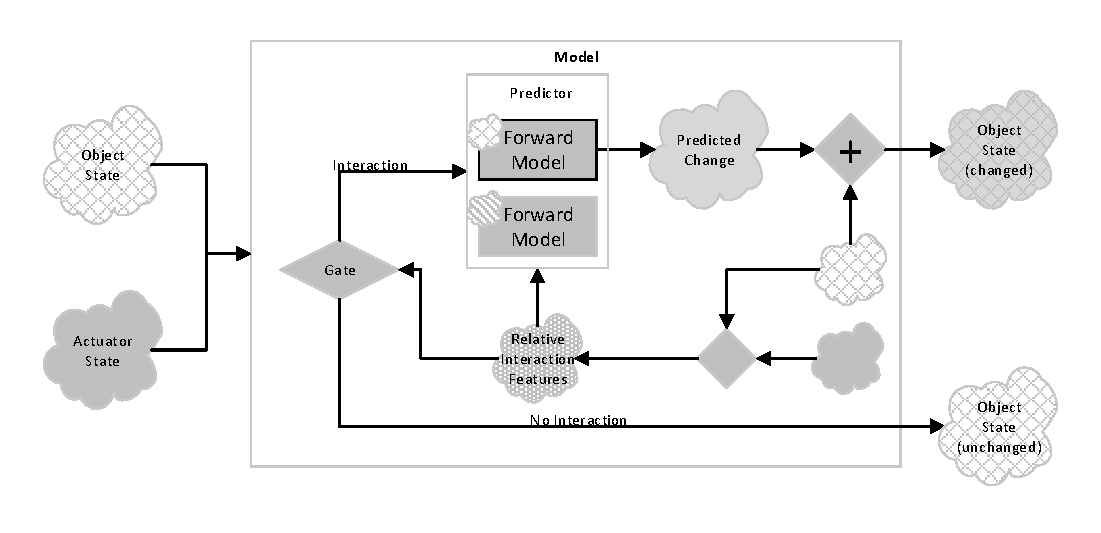
\includegraphics[width=\textwidth]{GatePrediction.pdf}
	\caption{Visualization of the prediction process for non actuator objects in the object space with gating concept. Using the predicted actuator state, relative interaction features are computed. These are used by the gating function to determine if an interaction takes place or not. The responsible local forward model is used to predict 
	changes in the object's state if an interaction is expected. From these changes the actual state prediction is computed.} 
	\label{fig:GatePrediction}
\end{figure}

First the next actuator state is predicted as mentioned above using the selected action primitive.
This predicted state is then used together with the current state of the object that is to be predicted to compute \textit{Relative Interaction Features}. These relative features are similar to the pairwise interaction state that was explained in the previous concept. However, since it is not necessary to extract the entire object states for both objects from these relative features, the dimensionality can be a lot lower than before. In fact, depending on the scenario, it may be sufficient to only represent the actuator in the local coordinate frame of the object. 
The gating function then uses these features to determine if the object will be influenced by the new actuator state. If the gating function predicts no interaction between the object and the actuator, the current object state is returned. 
On the other hand, if an interaction is predicted, the \textit{Predictor} uses the local forward model responsible for the current object. 
The local model predicts the changes in the object states instead of the final states. In order to get the actual predicted object state, these changes are added to the current object state.

When more than one object other than the actuator is present, the same process can be repeated. In order to predict interactions between two non actuator objects, a prediction chain is performed. First the actuator is predicted as described above. Afterwards, the objects that are directly influenced by the actuator are predicted. These predictions can then in turn be used as new \enquote{actuators} for interactions between them and other objects. %TODO consider removing this or moving this elsewhere since it is not done

%TODO decide which is used
%(STILL TO TRY) In order to predict multi object interactions, the gate function can be used to first collect all involved objects before
%invoking the appropriate predictor. (e.g. by interpolating the different input features).

\subsection{From target object state to action primitive \label{sec:gatePlanning}}

Similar to prediction, computing a suitable action primitive is performed differently depending on what kind of object is supposed to reach a given target configuration. In the case that the target object is the actuator, its inverse model is queried for an action primitive with the target configuration as input. 

The more interesting process of moving towards a target configuration for a non actuator object is visualized in figure \ref{fig:GatePlanning}.

\begin{figure}
	\centering
	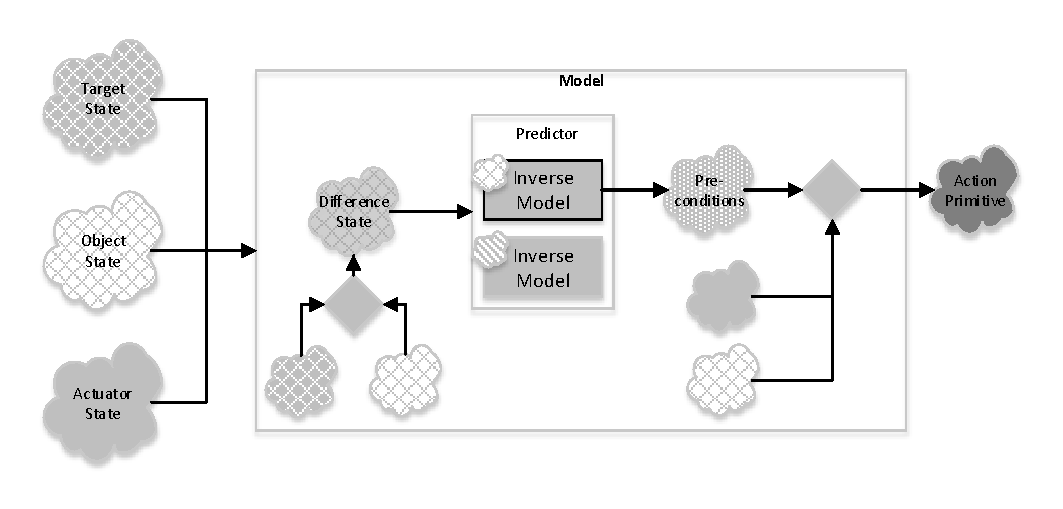
\includegraphics[width=\textwidth]{GatePlanning.pdf}
	\caption{Visualization of the process of computing action primitives to move non actuator objects to wards a target configuration in the object space with gating concept. Using the Difference State as input, the local inverse model queried for Preconditions. The resulting action primitive is computed from these preconditions.}
		\label{fig:GatePlanning}
\end{figure}
	
First the current difference state is computed from the given target configuration and the current object state. This difference state is then used to query the inverse model responsible for the target object. Since only the actuator can be influenced by action primitives directly, these local inverse models do not directly return action primitives. Instead they return preconditions in the form of the relative interaction features. These features represent a situation where the object state changes in the direction of the target configuration. 
	
The current actuator state is then compared to these preconditions. If the actuator is already in a configuration where it meets these preconditions, an action primitive is derived from the local features. This requires that the local features contain information that can be used to compute an action primitive.
However, in most situations the actuator configuration will not meet the preconditions. The given preconditions will often require the actuator to be in a different position relative to the object that is to be moved. In these cases the suitable position for the actuator is used as an intermediate target. 

Considering the current object's position, an action is calculated to move the actuator towards the intermediate target. This might result in a circling movement of the actuator around the object. Moving the actuator directly towards the intermediate target position might result in moving the object in a more unfavorable position and is therefore avoided. Since these steps are performed at every timestep, the model can quickly adapt itself to changes in the environment.
	
\subsection{Theoretical discussion}

Representing each object by itself has the advantage, that no transformations outside of the concept are required. Instead all objects are represented for themselves within the model. 
Consequently, any noise in any object does not directly influence another object's state. Noisy data in one object might still influence the prediction of another object, for example if the noise leads to an erroneous classification by the gating function. However, the effect is not as direct and unavoidable as in the pairwise interaction concept.

The big disadvantage of this approach is that impossible configurations can be predicted more easily. This can happen due to an inaccurate prediction made by either the actuator's or the object's forward model.
An impossible configuration is even bound to be predicted when the gating function misclassifies that no interaction takes place when it should. In this case the actuator is predicted to move into the other object.

Extending this concept to multiple objects is easier in theory since each object can be considered separately. However, training the gating functions with multiple objects is difficult. When one object's state changes during an update from the environment, the model needs to determine which other object caused this change in order to train the gating function on the correct relative interaction features. Depending on the situation, this determination can be very difficult and hardly be done without additional prior knowledge. 
%TODO example for such a situation?

Apart from the representation, this concept requires an additional assumption about the scenario compared to the interaction state concept. The assumption that object states can only change through interactions with an actuator also means that an object does not continue sliding after it has been pushed. This restricts the possible weights of the objects and speeds of the actuator.
%TODO rework/extend

\section{Time invariant inverse model \label{sec:invModel}}
%TODO other name!
%TODO soft introduction/"überleitung" von den anderen Kapiteln
Directly searching in the forward regression model for the inverse has two disadvantages in the given scenario: \\
1) The difference state that is computed can have features orders of magnitude greater than any change the local models have been trained with. In fact any target configuration, that requires multiple timesteps to reach, is already outside the range of the changes the forward models can have seen. 
The inverse model would need to extrapolate into unknown regions in these cases. \\
2) The features in the target state are not necessarily normalized. Therefore, the model does not necessarily know if a reduction of the difference in one feature is better than in another. This especially becomes a problem once only actions can be found that decrease the difference in one feature dimension at the cost of an increase in another feature dimension. Consider the example where a target position and orientation is given for an object. There might be situations where the object needs to be turned away from the target orientation in order to reduce the distance to the target position. In this case the orientation would need to be more or less ignored when using the inverse model to search for an action.

Furthermore, the output of the inverse model does not need to be as precise as the predictions of the forward model. This is mainly due to the fact that the inverse model is used to reach a target interactively. In the context of this thesis, there is no need to provide a sequence of precise action primitives that will then be executed blindly. Instead, as highlighted in figure \ref{fig:overview}, the model is tightly coupled with the environment. This means that the model is constantly updated and can adapt to changing situations. It is therefore sufficient for the inverse model to provide the means to make a step in the direction of the target configuration. In the context of the two concepts presented here, the means are not directly action primitives but rather preconditions that need to be fulfilled in order to be able to influence an object in a certain way.

In order to avoid the mentioned problems, a special inverse model is proposed that is trained separately from the forward model:
It is called \textit{\gls{tiim}} because, unlike a forward model, it does not focus on the actual quantity of the feature changes within one timestep. Instead, the inverse model focuses mainly on the direction, or the sign, of the changes. Furthermore, in order to avoid the problem of weighting feature importance, each feature dimension is considered separately. 

For each feature dimension, the model collects all the preconditions that result in a positive and negative change in that dimension separately. Here preconditions means a representation of the situation in which the change occurred.  
An example of this grouping is visualized in figure \ref{fig:InverseModel}. 

\begin{figure}
	\centering
	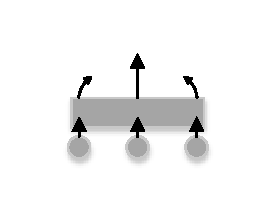
\includegraphics{InverseModel2.pdf}
	\caption{Visualization of the precondition grouping in the proposed time invariant inverse model. The arrows above the block symbolize the change in the object's state corresponding to the actuator situations below the block. All three pushing scenarios indicated by the three balls, will be grouped together since they all result in the same upward positional change.}
	\label{fig:InverseModel}
\end{figure}

The figure shows three different scenarios or preconditions in the form of the three balls that represent the actuator. In the forward model each precondition is tightly coupled to its resulting change. In this example the left situation results in the small positional change upwards and a negative change in orientation. The same tight coupling is present with the other two situations. In the inverse model proposed here, all three situations are grouped together in one \textit{prototype} responsible for a positional change upwards. Other prototypes exist for the two directions of change in orientation. This way one situation will be included in multiple prototypes if it has caused multiple features to change.

Each prototype creates a weighted average\footnote{depending on the used features, a simple average does not work. See the implementation details in section \ref{sec:invModelRealization} for details.} of the preconditions for its feature and sign. The preconditions are weighted by their contribution towards the feature. In the example above, the preconditions for the middle scenario receive the strongest weight since they are responsible for the biggest change in position. 

When the inverse model is queried given some difference vector to the target configuration a greedy strategy is used to reduce the feature with the biggest difference first. 
The feature along with the sign of this feature in the difference vector determine the responsible prototype. The average computed by that prototype can then be used as preconditions that will reduce the distance to the target configuration.



	

  \chapter{Model realization\label{chap:modelReal}}


%Detailed enough to be able to reproduce
%Pseudocode where applicable
%Explain along figure?
%Include technology that's used
%How did we realize/achieve the ideas?
%Present what kind of assumptions/prior knowledge is made!!

%\begin{itemize}
%	\item Actual architectures resemble concepts closely
%	\item Crux lies in the regression model (AITM)
%\end{itemize}
The previous chapter introduced two concepts that were develop with the goal of adapting themselves to unknown situations through interaction.
In order to evaluate the developed ideas, prototypes of the two concepts have been implemented in Python 2.7. Both prototypes are developed as such that they can be evaluated in the same way in the next chapter. The implementations follow the presented concepts very closely in most cases. As such the general data flow is the same as was presented in the figures  \ref{fig:PairPrediction}, \ref{fig:PairPlanning}, \ref{fig:GatePrediction} and \ref{fig:GatePlanning}.
Relevant implementation details as well as made assumptions are highlighted and explained in this chapter.

Section \ref{sec:basics} starts with describing common design decisions that apply to both concepts. Afterwards the relevant implementations details regarding the two prototypes are presented in section \ref{sec:pairRealization} for the interaction state concept and in section \ref{sec:gateRealization} for the object state concept. Finally, section \ref{sec:technologies} describes the used technologies, the underlying regression and classification model and the implementation of the inverse model, in detail.

\section{Basics \label{sec:basics}}

%The following descriptions and assumptions are accurate for all realizations independent of the underlying concept.
%TODO maybe rearrange the sentences

\subsection{Available information about objects}

The kind of information that is provided by the environment obviously depends on the sensors that are available to the robot. From the information provided by these sensors, features can be computed. The models themselves are greatly independent of what features are actually used. In fact the models do not require any knowledge about what the features represent for prediction. This allows the exact same model to be used in various settings with different features, for example if additional or different sensors are available. In order to yield good results, the used features obviously need to have the necessary expressiveness.

Unfortunately, the models do need to have some partial knowledge about the features when it comes to computing action primitives as will be further explained in the corresponding sections for both models.

These prototypes were evaluated using a physics simulation, further explained in section \ref{sec:environment}. From this simulation the information in table \ref{tab:availInformation} is provided for each object at each update.

\begin{table}[h!]
	\centering
	\begin{tabular*}{\textwidth}{@{\extracolsep{\fill} } l l}
		\textbf{Feature} & \textbf{Description} \\ 
		\hline \hline 
		x Position & Global x position of the object \\
		y Position & Global y position of the object \\
		Orientation & Global orientation around the z-axis of the object \\
		x Velocity & Global x velocity of the object \\
		y Velocity & Global y velocity of the object \\
		\hline 
	\end{tabular*} 
	\caption{Summary of all information about objects that is provided by the environment at each update step.}
	\label{tab:availInformation}
\end{table}

Furthermore, a unique identifier, the shape and size of the objects are known and can be used to compute additional features. What kind of features are computed from this information is a design decision by the user of these models. Since the underlying regression model is memory-based, using more features might result in worse performances. This is even more likely, if the features are not normalized or no suitable metric is used.

\subsection{Action primitives}

Action primitives are the collection of possible low level actions a robot can perform directly. Higher level actions are usually composed of multiple action primitives. For example, the action \textit{walking} might be composed of the action primitives \textit{raise leg} and \textit{lower leg}.

In the scope of this thesis, the action primitives are defined by the simulation used for the evaluations in the next chapter. In this case a two dimensional action primitive is used, representing the $x$ and $y$ velocity of the actuator. The velocities are given according to the global coordinate system of the robot. 
In general, the nature of the action is not all that important to the models as long as it can be represented as a vector. 
However, the models assume that an action primitive is selected and performed at every iteration. This is also true for the used velocity action primitives, even if the velocity does not change by using the same action primitive again. 

The used simulation only accepts velocities with a norm not higher than $0.5\frac{m}{s}$. The implementations make sure to scale all computed action primitives accordingly. While moving towards a target, the implementations scale the action primitives to a norm of $0.3\frac{m}{s}$ in order to not push the objects too far.

\subsection{Used regression and classification model}

As already stated in the introduction and motivated in chapter \ref{chap:stateOfTheArt}, this thesis uses a memory-based approach to learn the interactions. For this end, a special adaptation of the \gls{gng} has been developed which can be used for regression as well as classification tasks. This adaptation, called \acrfull{aitm} and explained in section \ref{sec:ITM}, is used for all regression and classification models used in both prototypes unless stated otherwise. 

\subsection{Using local features and predicting differences \label{sec:localFeatures}}

Both prototypes only use local (differential) features as inputs for their trained regression and classification models. 
Local features mean that all features are represented relative to some reference object's coordinate frame. The exact computation of the features is explained in sections \ref{sec:intFeatures} for the interaction model and \ref{sec:gateFeatures} for the object state model.
Using local features assumes that similar interactions behave identical regardless of where they take place in the environment. 
Only the local relations between the involved objects determine the outcome of the interaction. 
For the given task of pushing interactions this assumption will hold true as long as the environment only has constant effects on the objects. The environment used for the evaluations, described in section \ref{sec:environment}, fulfills these conditions since it only affects the objects through gravity and friction, which are constant in the given scenario. 

The great advantage of this approach is that the interactions can be learned regardless of the object's actual configuration in the environment. In fact training data from all configurations can be used to learn a certain interaction. Furthermore, this approach provides free generalization to any configuration in the environment without the need of additional training data.

In more realistic environments, where this assumption does not hold true, the local features can still be used. However, in this case, additional features containing the information about the influence of the environment or the current object configuration might be required. Depending on the actual scenario and its dynamics, this might require absolute global features which offer a lot less generalization.

An additional consequence of these local features is that the forward models of both concepts can only predict the changes instead of resulting features. As already stated in the two concept descriptions, the actual predictions for the interaction state and the object state are computed by adding these predicted changes to the current states.
Without knowledge about the actual position in the input data, the actual position after an interaction cannot be predicted. However, this is not a problem but rather a benefit. Changes are limited in their size compared to the resulting features. 
Consider the feature position: An object cannot change its position from one timestep to another arbitrarily, but rather only by a certain maximum amount. When predicting changes, the learner's output only needs to cover the subspace defined by this maximum amount instead of the entire space. Furthermore, this approach of only predicting the changes can also be applied when using global input features. The models themselves are therefore not restricted by this.


\section{Modeling pairwise interaction \label{sec:pairRealization}}

The implementation of the pairwise interaction model contains the components visualized in the overview figure \ref{fig:PairOverview}.
The \acrfull{acs} trains a classifier that selects any of the $n$ learned \glspl{ac}. Within each \glspl{ac}, there exist a local forward model which performs the predictions.
However, instead of training local inverse models for each \gls{ac}, one global inverse model is used in this implementation. The reasons for this decision are explained in section \ref{sec:pairPlanningReal}.
Just as the local ones would, the global inverse model returns preconditions that result in a specific change of the interaction state.
The forward model as well as the selector both use the same underlying mechanism in the \acrfull{aitm}. For the reasons explained in section \ref{sec:invModel}, the special \acrfull{tiim} is used for the global inverse model.

As mentioned before, the model is constantly updated with new information provided by the environment. The steps that are performed to update the model each time new information is received are explained in algorithm \ref{alg:intUpdate}.

\begin{algorithm}
\begin{algorithmic}[1]
	\Require{New worldstate ws}
	\Require{Used action $act$}
	\Data{Last worldstate ws$_\text{old}$}
	\Data{Set of Abstract Collections L}
	\Data{Inverse Model IM}
	\Data{Abstract Collection Selector ACS}
	\Statex
	\ForAll{interaction state i $\in$ ws}
		\Let{i$_\text{old}$}{extractInteractionState(ws$_\text{old}$, i)}
		\Let{newEpisode}{Episode(i$_\text{old}$, $act$, i)}
		\Let{$S$}{computeChangedFeatures(newEpisode)}
		\If{$S$ $\notin$ L} \Comment{Check if a corresponding AC already known} 
			\Let{newAC}{AbstractCollection($S$)}
			\Let{L}{L $\cup$ newAC}
		\EndIf
		\Let{AC}{L$_S$} \Comment{The Abstract Collection responsible for $S$} 
		\State update AC with newEpisode
		\State update IM with newEpisode
		\State update ACS with i$_\text{old}$, $act$ and AC
	\EndFor
\end{algorithmic}
\caption{Prediction of the update steps in the pairwise interaction model.}
\label{alg:intUpdate}
\end{algorithm}

%\begin{algorithm}
%	\KwIn{New worldstate ws}
%	\KwIn{Used action $act$}
%	\KwData{Last worldstate ws$_\text{old}$}
%	\KwData{Set of Abstract Collections L}
%	\KwData{Inverse Model IM}
%	\KwData{Abstract Collection Selector ACS}
%	\BlankLine
%	\ForEach{interaction state i $\in$ ws}{
%		i$_\text{old}$ = extractInteractionState(ws$_\text{old}$, i)
%		newEpisode = Episode(i$_\text{old}$, $act$, i) \\
%		$S$ = computeChangedFeatures(newEpisode) \\
%		\tcc*[h]{Check if a corresponding AC already known} \\
%		\If{$S$ $\notin$ L}{
%			newAC = AbstractCollection($S$) \\
%			L = L $\cup$ newAC 
%		}
%		AC = L$_S$ \tcc*[f]{The Abstract Collection responsible for $S$} \\
%		update AC with newEpisode \\
%		update IM with newEpisode \\
%		update ACS with i$_\text{old}$, $act$ and AC
%	}
%	\caption{Prediction of the update steps in the pairwise interaction model.}
%	\label{alg:intUpdate}
%\end{algorithm}

The changed feature set $S$ is computed according to equation \ref{eq:difSet}\footnote{Since local features are used, both $Pre$ and $Post$ need to be transformed to the same coordinate frame, see section \ref{sec:episodes} for details.}. The structure and used features within the interaction state are explained in section \ref{sec:intFeatures} while the episodes are explained in section \ref{sec:episodes}.

When updating an \gls{ac} its forward model needs to be updated. The forward model is trained using the combination of the old interaction state  i$_\text{old}$ and the action primitive $act$ as input and the difference vector $\vec{d}$ between the old and the new interaction state as desired output. The exact training of the \gls{aitm} is explained in section \ref{sec:ITM}. 

The global inverse model is trained on the same features as the forward model. The exact process behind the training is explained in section \ref{sec:invModelRealization}.

The \gls{acs} is also trained on the same combination of i$_\text{old}$ and $act$ as input, but it uses the identifier of the responsible \gls{ac} as desired output.
Since the selector also uses the \gls{aitm} as classifier, the exact update rules are explained below.

When used for prediction the model follows the process visualized in figure \ref{fig:PairPrediction} and described in section \ref{sec:pairPrediction}.
Computing suitable action primitives on the other hand is more complicated and requires additional knowledge about the features. While the general process follows what is explained in \ref{sec:pairPlanning}, the process of providing relevant interaction states as targets and extracting relevant action primitives from the returned preconditions is explained in section \ref{sec:pairPlanningReal}.

%The model itself only works on interaction states and action primitives. The specific structure and content of these features is explained in section \ref{sec:intFeatures}.


\subsection{Used features \label{sec:intFeatures}}

The pairwise interaction model basically only uses the interaction state and the action primitive vector as feature vectors. The actual composition of the interaction state depends on the objects that need to be represented. For this thesis, only simple objects (e.g. spheres or rectangular cubes) are present in the scene which allow fairly simple interaction states as described in table \ref{tab:pairInteractionFeatures}.

\begin{table}
	\centering
	\begin{tabular*}{\textwidth}{@{\extracolsep{\fill} } l l}
		\textbf{Feature} & \textbf{Description} \\ 
		\hline \hline 
		 Id 1 & Identifier of the reference object \\ 
		 Id 2 & Identifier of the second object \\ 
		 Local x Position & Local x position of the reference object \\
		 Local y Position & Local y position of the reference object \\
		 Local Orientation & Local orientation of the reference object \\
		 Relative x Position & Relative x position of the second object \\
		 Relative y Position & Relative y position of the second object \\
		 Relative Orientation & Relative orientation of the second object \\
		\hline 
	\end{tabular*} 
	\caption{Features used to represent one interaction state. Relative positions and velocities refer to the coordinate system of the reference object.}
	\label{tab:pairInteractionFeatures}
\end{table}

As already mentioned in section \ref{sec:localFeatures} differential features are used. Apart from the features listed in the table, the interaction state contains the information required for the transformations. Specifically, the matrix $T$ used to transform from the local coordinate frame back to the global frame, its inverse $T^{-1}$ and the orientation of the reference object in the global coordinate frame are stored.

The model assumes, that these interaction states come directly from the environment. Transformations from and to the actual object states need to be performed outside of the actual model. This is achieved by introducing a \textit{Worldstate}. From the point of view of the model, this worldstate is simply a collection of all interaction states in the environment. At each update from the environment, a new worldstate is computed from the provided information. The model predicts a new worldstate by making predictions about all interaction states that are included in a given worldstate. Since one is usually more interested in the actual object states, the model finalizes the worldstate after all interaction states have been predicted. This finalization extracts the object state predictions from the predicted interaction states. 

The interaction states are computed as follows:
All features are computed by transforming the global features of both objects given by the environment to the local coordinate frame. Consider two objects $o_1$ and $o_2$ with positions $\vec{p}_1$ and $\vec{p}_2$ and orientations $\alpha_1$ and $\alpha_2$ respectively. First the transformation matrices $T$ and $T^{-1}$ are computed from the reference object's position and orientation:

\begin{equation}
T = \begin{pmatrix}
\cos(\alpha_1) & -\sin(\alpha_1) & p_{x1} \\
\sin(\alpha_1) & \cos(\alpha_1) & p_{y1} \\
0.0 & 0.0 & 1.0
\end{pmatrix}
\qquad
T^{-1} = inv(T)
\label{eq:transMatrix}
\end{equation}

$p_{x1}$ and $p_{y1}$ correspond to the $x$ and $y$ dimensions of the position $\vec{p}_1$. With the help of the transformation matrix $T^{-1}$ it is possible to compute the local positions, e.g.:

\begin{equation}
\vec{p}' = T^{-1} \times \vec{p}_1^*
\end{equation}

where $\vec{p}_1^*$ is the homogeneous vector of $\vec{p}_1$. Since $\vec{p}'$ is also in homogeneous coordinates, only the first two components are used for the interaction state. The local and relative orientations are computed by subtracting the orientation of the reference object from the given orientations. In fact by doing this, all local fields in the interaction state will be zero after the computation. However, these fields are still required. The \glspl{ac} predict the change in the current interaction state. In order to extract the predicted object states from the interaction state, changes in the reference object need to be predicted as well. 

The object states are extracted by using the inverse transformation. Since the structure of the interaction states are known outside of the model, the predicted local position $\vec{q}$ can easily be extracted. Using the homogeneous coordinates $\vec{q}^*$ of $\vec{q}$, the prediction for the actual object's position $\vec{p}_{pred}$ can be computed:

\begin{equation}
\vec{p}_{pred}^* = T \times \vec{q}^*
\end{equation}

Velocities can be computed analogously if needed.
In order to get the global orientation, the reference object's orientation simply needs to be added to the predicted orientation. 

\subsection{Episodes \label{sec:episodes}}

Episodes are used to store past experiences. The idea comes from case-based-reasoning \cite{cbr} where past experiences are used to reason about new problems. An episode is made up of three parts: 
\begin{enumerate}
\item The initial interaction state $Pre$ that was given before an action was performed.
\item The action that has been performed.
\item The resulting interaction state $Post$.
\end{enumerate}

As explained in the concept, these experiences can be stored and looked up at query time in order to make predictions. However, as highlighted before, the performance of such an operation deteriorates over time as the number of stored experiences increases. Instead, the \glspl{ac} use these episodes as training data for the local regression model. Apart from those three parts, all episodes compute a difference vector between the initial and resulting interaction state. 
However, since the model is working with local coordinates, it is important that both states are transferred to the same coordinate frame before computing the difference. As explained above, the features in all interaction states are always computed relative to the reference object's coordinate frame. As such the positional information of the reference object will always be zero in a freshly computed interaction state. However, this does not mean, that the reference object has not moved within an episode. The model is interested in learning to predict how a given interaction state changes after a special action is performed. Therefore, the difference vector in an episode needs to represent the differences relative to the initial interaction state. This is achieved by first transforming the features of the $Post$ state back to global coordinates via $T_{Post}$ and then transforming them to the local coordinate frame of the $Pre$ state using $T^{-1}_{Pre}$. For the position of the reference object $p_{ref}$ (in homogeneous coordinates) this can be computed as follows:

\begin{equation}
\vec{p}'_{ref} = T^{-1}_{Pre} \times T_{Post} \times \vec{p}_{ref}
\end{equation}

When transforming the orientation of the $Post$ state, first the global orientation of $Post$'s reference object is added before subtracting $Pre$'s global orientation. All transformed features from $Post$ are again collected in a vector $Post^*$ where the features are organized in the same way as in a normal interaction state.

Afterwards the difference vector can simply be computed by:

\begin{equation}
\vec{d} = Post^* - Pre
\end{equation}

During training, the \glspl{ac} extract the feature differences that they are responsible for from $\vec{d}$ and use those as target output of the local regression model.
Finally, the set of changing features $S$ can then again be computed as stated in equation \ref{eq:difSet} while substituting $Post$ with $Post^*$.

\subsection{From target object state to action primitives\label{sec:pairPlanningReal}}

In most cases the robot will have to push a certain object to a given specification. It usually does not matter where the actuator is after the target is reached. Therefore, it would be best if a target object state could be provided instead of a target interaction state. However, the model itself does not know about object states. Therefore, this prototype implements a method to convert a given object state to an interaction state, where only the reference object is correctly set. The actuator is used as secondary object, however the actuator's features are not required. Instead, the features representing the reference object are remembered in order to only focus on these features when trying to reduce the distance to the target interaction state. 

Once a target interaction state has been computed, the current interaction state between the reference object of interest and the actuator can be retrieved. Using the target interaction state as resulting state, an episode with an empty action is computed. The episode provides the difference vector between the current situation and the target configuration. Only the features remembered when constructing the target interaction states are considered from this difference vector. Effectively, these features correspond to the local differences in the object states. 

Following the concept provided in section \ref{sec:pairPlanning}, this reduced difference vector would be used to find the \gls{ac} that is responsible for changes represented in the vector.
Having said that, since only changes of a subset of the entire interaction state are considered, there will usually not be an \gls{ac} that is responsible exactly for these changes. 
Instead there will be several \glspl{ac}, that are responsible for changes in these features. In theory, the \gls{ac} responsible for the most feature changes should be chosen in this situation. 

Unfortunately, the developed inverse model does not work well with the segmentation performed by the \glspl{ac}. The main reason for that is, that the inverse model trains separate prototypes for each feature dimension.
Each prototype tries to learn the preconditions that have the most influence on the given feature dimension. A single feature dimension is often represented in multiple \glspl{ac}. Therefore, each local inverse model would only experience a subset of the preconditions responsible for changes in a specific feature dimension. When the \gls{tiim} is trained only on these local parts, the prototypes do not learn the preconditions well.

On top of that, the \gls{tiim} is a model with close to constant update and query times\footnote{The number of prototypes and averages that are learned per prototype are independent of the number of training examples. See section \ref{sec:invModelRealization} for details.}. Therefore, the main reasons for training multiple local models do not apply to this inverse model.

It is for these reasons, that this implementation deviates from the concept in this point and only trains a single global inverse model.
This global inverse model is queried just as a local one would be and returns suitable preconditions given a difference vector.

Once preconditions have been retrieved from the inverse model, the current situation is compared to these preconditions. Most importantly, the current actuator position needs to be similar to the actuator position in the preconditions. If the distance between these two positions is too great, the actuator is circled around the object. Unfortunately, this requires some world knowledge about the objects. In the given implementation, the interaction states defined by the user provide the ability to compute an action primitive that lets the actuator circle around the reference object at a fixed distance (see Appendix \ref{sec:circling} for details). 
Using this circling action the actuator is able to move towards the desired position without influencing the object.

Once the distance is below a threshold of 0.1m\footnote{The threshold heavily depends on the given environment and the size of the objects. This threshold has been empirically determined and worked well in the evaluation environment described in section \ref{sec:environment}.}, the model assumes that the actuator is on the correct side of the object and can move directly towards the desired position. This can be done by simply following the direction between the target position and the current position.

Once the actuator has come close\footnote{This implementation uses the threshold of 0.01 to determine when it is close enough.} enough to the position defined by the preconditions, the actual desired action primitive can be computed. The preconditions already contain local action primitives that were encountered during training. These can be transformed to the global coordinate frame using the transformation matrix $T$ from the current interaction state as described above. 


\section{Object space with gating function \label{sec:gateRealization}}

The realization of the second prototype consists mainly of the parts visualized in figure \ref{fig:GateOverview}. 
Depending on whether the actuator models are to be learned as well, three to five different parts need to be trained in this model: The predictor occupies a similar role to the \glspl{ac} in the previous model. For each distinct object group, a local forward model is trained using the relative interaction features (described in section \ref{sec:gateFeatures}) as input and the changes in the object states as output. Just as the interaction model, the inverse model is also trained on the same input and output data each time new information is available from the environment. 
In this implementation, object groups are simply divided by the object identifier. 
The gating function trains a classifier in order to predict if an actuator object influences another object. The classifier is trained, using the relative interaction features as input. The output, i.e. if an interaction took place or not, is determined by computing the change between the previous object state and the current one.

Algorithm \ref{alg:gateUpdate} summarizes all steps performed at each update step.

\begin{algorithm}
\begin{algorithmic}[1]
	\Require{New worldstate ws}
	\Require{Used action $act$}
	\Data{Last worldstate ws$_\text{old}$}
	\Data{Predictor}
	\Data{Gate}
	\Statex
	\Let{newActuator}{extractActuator(ws)}
	\State updateActuator(newActuator, $act$)
	\ForAll{object state o $\in$ ws}
		\Let{o$_\text{old}$}{extractObject(ws$_\text{old}$, o)}
		\Let{relFeatures}{computeRelativeFeatures(o$_\text{old}$, newActuator)}
		\Let{change}{computeLocalChange(o$_\text{old}$, o)}
		\Let{hasChanged}{$||$change$|| > \epsilon_{change}$}
		\State updateGate(relFeatures, hasChanged)
		\If{hasChanged}
			\State updatePredictor(relFeatures, change)
		\EndIf
	\EndFor
\end{algorithmic}
\caption{Summary of the steps performed by the object state model at each update from the environment.}
\label{alg:gateUpdate}
\end{algorithm}


%\begin{algorithm}
%	\KwIn{New worldstate ws}
%	\KwIn{Used action $act$}
%	\KwData{Last worldstate ws$_\text{old}$}
%	\KwData{Predictor}
%	\KwData{Gate}
%	\BlankLine
%	newActuator = extractActuator(ws) \\
%	updateActuator(newActuator, $act$) \\
%	\ForEach{object state o $\in$ ws}{
%		o$_\text{old}$ = extractObject(ws$_\text{old}$, o) \\
%		relFeatures = computeRelativeFeatures(o, newActuator) \\ 
%		change = computeLocalChange(o$_\text{old}$, o) \\
%		hasChanged = $||$change$||$ > 0 \\
%		updateGate(relFeatures, hasChanged) \\
%		\If{hasChanged}{
%			updatePredictor(relFeatures, change) \\
%		}
%	}
%	
%	\BlankLine
%\caption{Algorithm summarizing the steps performed by the object state model at each update from the environment.}
%\label{alg:gateUpdate}
%\end{algorithm}

At the beginning of each update step, the current and last states for the actuator as well as the objects is retrieved from the current and last worldstate respectively.
Extracting the actuator or an object state is simply an attribute lookup in the worldstate. 

The actuator is updated first. If no local forward and inverse models are predefined, an \gls{aitm} is updated with the used action primitive as input and the change in the actuator's state as output.

Afterwards each object is considered separately. The object's change needs to be computed. Since the local models want to predict local changes, the change in an object's state needs to be computed with respect to the coordinate frame before the update. This requires the features to be transformed as described in section \ref{sec:gateFeatures}.

Furthermore, the relative interaction features between the old object state and the new actuator state need to be computed. The new actuator state is used because the model uses the predicted actuator state when making predictions instead of the current one. Therefore, the model needs to train using actuator state that results from the last action primitive, instead of the old actuator state.

The computed change is used to determine if the current object has actually changed by comparing the norm of the change with $\epsilon_{change}$. This threshold should be set according to the noise level in the received information. This implementation uses $\epsilon_{change} = 0$.

When the object state has changed, the predictor is updated with the relative interaction features as input and the change as output. In this implementation the predictor determines the object group by the identifier in the relative features in order to train only the local forward and inverse models responsible for the current object group. Ideally, the model would be able to automatically determine object groups through interaction and comparing their behavior.

When used to predict the next world state, the process visualized in figure \ref{fig:GatePrediction} and described in section \ref{sec:gatePrediction} is used for every object in the current worldstate. As mentioned in the concept, prediction is a sequential process in this model: \\
First the next actuator state is predicted by querying its local forward model given the selected action primitive. The predicted actuator state is then used to compute the relative interaction features with the current object. This feature vector is then used to query both the gate and if required the object's local forward model in the predictor. 
As a consequence of this sequential process, the local models in the predictor do not know about the action primitives at all. %TODO explain benefits of this

As in the other model, computing action primitives is more complicated and requires additional knowledge about the features. The steps required to extract action primitives useful to reach a given target are explained in section \ref{sec:gatePlanningReal}

\subsection{Used features \label{sec:gateFeatures}}

Similar to the interaction model, this model also introduces a \textit{Worldstate}. This worldstate is computed at each update from the environment. In this case, the worldstate simply collects the states of all objects in the environment. The actuator, although technically an object, is regarded separately in the worldstate. Since the model directly predicts the new object states, no finalization is required. 
The object states describe the specific features of each object and basically represent what is provided by the environment. This implementation can use dynamic features such as velocities, but does not require them. Table \ref{tab:gateObjectFeatures} summarizes the basic features that are used to represent object states.

\begin{table}
	\centering
	\begin{tabular*}{\textwidth}{@{\extracolsep{\fill} } l l}
		\hline \textbf{Feature} & \textbf{Description} \\ 
		\hline \hline 
		 Id & Unique identifier of each object \\
		 x Position & Global x position in the environment \\ 
		 y Position & Global y position in the environment \\ 
		 Orientation & Object rotation around the z-axis of the global coordinate system \\ 
		\hline 
	\end{tabular*} 
	\caption{The different dynamic features used to represent objects.}
	\label{tab:gateObjectFeatures}
\end{table}

While additional information, such as information about the shape of the objects, is available, the model itself does not require it. However, when computing the relative interaction features, at least information about the shape is required. Furthermore, the model stores not only the current state of each object but also the previous one. This is required in order to make finite difference estimations about the objects dynamics such as velocity. 
In case the dynamics are directly provided by the environment, this previous state does not need to be stored. However, omitting the velocities and only estimating them when needed reduces the output dimensionality of the regression models. This is because the model predicts changes in all features that it experiences. Since the model does not have or require any knowledge about the features for prediction, a selective prediction is not possible. Therefore, it is beneficial to reduce the number of features that need to be predicted. 

The different regression and classification models are trained using relative interaction features as input. As mentioned in the concept description, these features are similar to the interaction state described in the pairwise interaction model above. However, not all information about both objects needs to be expressed. This is because, the each object's information is available. Furthermore, as mentioned before, the model assumes that the global configuration of an object does not influence an interaction.  Therefore it is sufficient to model the actuator relative to the reference object. Additional information that might be useful for the learner is also provided.
The relative interaction features are summarized in table \ref{tab:gateInteractionFeatures}. 

\begin{table}
	\centering
	\begin{tabular*}{\textwidth}{@{\extracolsep{\fill} } l l}
		\hline \textbf{Feature} & \textbf{Description} \\ 
		\hline \hline 
		 Id 1 & Identifier of the reference object \\ 
		 Id 2 & Identifier of the second object \\ 
		 Distance & Closest distance between the two objects \\
		 Closing & Describes how much the objects are moving towards each other \\
		 Relative x Position & Relative x position of the second object \\
		 Relative y Position & Relative y position of the second object \\
		 Relative x Velocity & Relative x velocity of the second object \\
		 Relative y Velocity & Relative y velocity of the second object \\
		\hline 
	\end{tabular*} 
	\caption{The different relative interaction features used to make predictions about interactions. Relative positions and velocities refer to the coordinate system of the reference object.}
	\label{tab:gateInteractionFeatures}
\end{table}

The \textit{Closing} feature $c$ is visualized in figure \ref{fig:closing}. Its computation is given by equation \ref{eq:closing}.

\begin{equation}
  c = \vec{n} \cdot \vec{rv}
 \label{eq:closing}
\end{equation}

$\vec{n}$ represents the normal vector from the reference object towards the second object and $\vec{rv}$ represents the non normalized relative velocity vector of that second object. This equates to the cosine between these two vectors weighted by the magnitude of the relative velocity. This feature is minimal when the objects are moving directly towards one another. A positive closing value on the other hand indicates that the objects are moving away from each other. When the feature becomes 0 it indicates that the distance will not change. As mentioned above, the relative velocity is estimated by the finite difference of the current and last position.

\begin{figure}
	\centering
	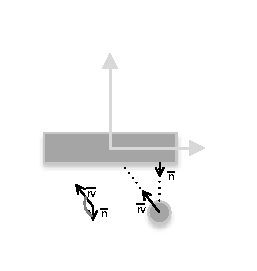
\includegraphics[scale = 1.5]{closing.pdf}
	\caption{Visualization of the closing feature. The gray half circle shows the angle whose cosine is basically computed for the feature.} 
	\label{fig:closing}
\end{figure} 

The other relative features are computed by transforming their global counterparts to the coordinate system of the reference object. Equation \ref{eq:trans} shows this exemplary for the position:

\begin{equation}
	\vec{relPos} = T^{-1} \times \vec{gPos}
\label{eq:trans}
\end{equation}

where $T^{-1}$ is the transformation matrix computed from the reference objects orientation and global position as defined by equation \ref{eq:transMatrix}. $\vec{gPos}$ is the position vector of the second object in homogeneous coordinates. The same transformation is required when computing the change in an object's state. 

The distance is calculated by computing the distances from all corners of one objects to all edges of the second object. 
The distance between the two objects corresponds to the closest of these corner-edge distances. In case of round objects, such as the actuator, the center is considered as a corner and the radius is subtracted from the computed distance.


\subsection{From target object state to action primitive \label{sec:gatePlanningReal}}

The overall process of computing a suitable action primitive that allows to push an object towards a given target configuration is quite similar to the one in the previous model that is explained in section \ref{sec:pairPlanningReal}. However, due to the differences in representation, the process is actually easier in this model. 
First of all, since the model works directly with the object states, the target representation does not need to be changed. A specified target object state can directly be used by the model. 
Furthermore, for each object group only one inverse model exist, which directly avoids the problems with multiple local inverse models mentioned in section \ref{sec:pairPlanningReal}. 

The preconditions are computed as visualized in figure \ref{fig:GatePlanning}: \\
First the difference vector between the current object state and the target state is calculated. Afterwards, the local inverse model responsible for the given object is queried for the preconditions given this difference vector. The actual computation of these preconditions is explained in section \ref{sec:invModelRealization}.

Once the preconditions have been computed, the same analysis as in the other model needs to be performed. These preconditions are in the form of the relative interaction features described above.
Unlike in the prediction case, the model needs to have knowledge about what some of the features represent. Specifically, the information about the local actuator position $\vec{p}_{cond}$ needs to be extracted from these preconditions. Afterwards, $\vec{p}_{cond}$ can be compared with the local actuator position $\vec{p}_{cur}$. $\vec{p}_{cur}$ is extracted from the current relative interaction features between the object and the actuator. 
If these two positions are too far apart\footnote{This implementation considers an euclidean distance of 0.1 as too far apart. This threshold has proven to be suitable in the environment presented in section \ref{sec:environment}.} a circling action is performed. Unfortunately, this needs to be provided by the user since the model has no information about the shape of the objects or what circling means. In this implementation, each object state, that needs to be defined by the user anyways, provides a method that computes an action that circles the actuator around the object in a fixed distance.
The exact algorithm used to compute the circling action is given in Appendix \ref{sec:circling}.

The model uses a circling action instead of directly moving towards the desired position, because the target position might be on another side of the object. When moving the actuator straight towards $\vec{p}_{cond}$ the object might be influenced in a negative way.

If the actuator is close but not close enough\footnote{This implementation considers a euclidean distance of < 0.01 as close enough.} the direction $\vec{d} = \vec{p}_{cond} - \vec{p}_{cur}$ can be used as action primitive.
However, regardless of how fine the \enquote{closeness} threshold is set, the object might still be in the way of this direction in some cases. In order to avoid, moving the object in an unintended way, the direction is only followed if the gate predicts that the next action will not influence the object. Otherwise, the same circling movement as described above is performed.

Once the actuator is close enough to $\vec{p}_{cond}$, the actual action primitive needs to be extracted from the preconditions. 
While the action primitives were directly included in the preconditions in the interaction model, they are not included in the preconditions for this model. 
However, the relative interaction features include the relative velocity of the actuator. 
Since the action primitives control velocities in this scenario, the direction of this relative velocity can be used to construct an action primitive that points in the same direction. Afterwards, the action primitive needs to be transformed to the global coordinate frame, using the transformation matrix $T$ as explained above.

\section{Used technologies \label{sec:technologies}}

\subsection{The Averaging Inverse Model \label{sec:invModelRealization}} 

The \acrfull{tiim} was suggested in the previous chapter in order to deal with the problems involved in computing the input from a given output. In this setting, the problem of extrapolation is the most important one since the models are supposed to reach any target not ones that are reachable by performing a single action primitive.

This special inverse model is designed to learn typical preconditions that result in a certain change in the features. It is less important how strong the change is, but rather in what direction (positive or negative) a feature dimension changes. The idea is to compute the average preconditions for each feature dimension and each direction this dimension changes in. This assumes, that similar situations result in similar changes, for example if a block is pushed from the left it moves to the right.
 
These preconditions depend on the actual model. In case of the interaction model, the combination of interaction state and action primitive is used while the object state model used the relative interaction features. However, as described above, this average can be used to derive an action primitive in both cases.

The implementation of this inverse model consists of two parts: 
\begin{itemize}
\item A \textit{network}
\item Its nodes (\textit{prototypes})
\end{itemize}

\textbf{Network:}

The network is the main part of the inverse model. It contains and manages the different prototypes. 
As explained in the sections for both models, the inverse model is trained on the preconditions and the difference vector. The difference vector $\vec{d}$ represents either the changes in an interaction or an object state depending on the used model.

For each actually changing feature dimension within $\vec{d}$ the network creates up to two prototypes. One for positive and one for negative changes within that dimension. That way a prototype represents changes in a given direction (positive or negative) of one specific feature dimension. 

In the example in figure \ref{fig:InverseModel} three different pushing interactions between the actuator and an object are seen. 
When the network is trained on these situations, three prototypes are created: One for the position change upwards and one for each rotation direction. 
Since all three situations result in an upward positional change, the corresponding prototype averages the preconditions of all three situations.
On the other hand, the two orientation prototypes will only be trained on one situation each.

The network is queried to provide preconditions that reduce a given difference vector. Ideally, preconditions that reduce the difference in all features at the same time would be returned. 
However, averaging the preconditions returned by different prototypes is prone to produce invalid preconditions. 
Furthermore, depending on the environment, it might not always be possible to reduce all features at the same time. 

In order to avoid invalid preconditions, the network uses a greedy strategy of reducing the feature dimension with the biggest difference\footnote{In order to avoid oscillations between different features and preconditions, the network remembers the selected feature until the sign in the difference flips or the feature difference $||f|| < \epsilon_{Index}$. Again this threshold depends on the expected change of features in the environment.}. Since the feature dimensions are not normalized, the biggest numerical value might not correlate to what humans regard as a big distance. 
However, this approach works quite well in practice, considering the inverse model does not have any knowledge about the feature's characteristics. 

Once the feature dimension with the biggest difference has been chosen, the corresponding prototype returns up to two possible preconditions as explained below.
The prototypes are asked to return two preconditions where possible in order to allow greater flexibility of the network: \\
The network tries to determine preconditions that reduce the difference in the biggest feature dimension while also setting up future movements in order to reduce the next biggest difference. Consider the example in figure \ref{fig:avgProblem} where two valid alternative preconditions are visualized: If the block should not only be rotated counterclockwise but also moved upwards, the position below the block is more favorable. This is because, in order to reduce the positional difference, the preconditions averaged over the situations visualized in figure \ref{fig:InverseModel} would be used. On the other hand, if the block should be moved to the right, the other situation should be preferred.

In order to do that the network queries the preconditions for the second biggest feature dimension as well. By comparing the (euclidean) norms between the four preconditions it is possible to determine which of the two preconditions for the first feature dimension is closer to the preconditions of the second feature dimension.  

In case both alternatives for the first feature are deemed equally good, the first preconditions are used since these correspond to a greater change in the desired feature dimension.

Unfortunately, this strategy, does not always avoid choosing the suboptimal preconditions. Since the preconditions for the second biggest feature dimension can only ever be evaluated based on the current situation, wrong choices might be made. Consider the same example as above, but the block is supposed to be turned by 180°. In that case, the local positional difference, the inverse model tries to reduce, will change its sign by turning the block around. This means that in order to move the block upwards in the global sense after turning it around, the block needs to be pushed downwards regarding its local coordinate system. In this case, the alternative above the block would have been the better choice.

\textbf{Prototype:}

Within a prototype, all collected preconditions are averaged by weighting each input by the magnitude of the change in the feature dimension in $\vec{d}$ that the input caused.
In the example in figure \ref{fig:InverseModel}, the middle scenario receives the biggest weight, since it changes the position more then the outer situations. 

While this average works great in the given example for the positional node, it does not work for all features as can be seen in figure \ref{fig:avgProblem}.

\begin{figure}
	\centering
	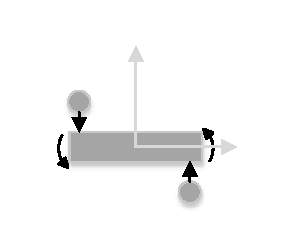
\includegraphics{avgProblem.pdf}
	\caption{Visualization of two alternative preconditions for a positive rotation of the block. The circles represent the actuator while the rectangle represents a block object. The gray arrows symbolize the local coordinate system of the block. Averaging these preconditions in the prototype would result in an invalid precondition.} 
	\label{fig:avgProblem}
\end{figure}

Consider the orientation prototype for positive rotations around the z-axis as shown in the figure. The magnitude of the change is identical in both situations, meaning that normally, the mean of both preconditions should be used as the average. In the given situation, this results in invalid preconditions, where the actuator would be supposed to be in the center of the object. That position is not only not reachable, but it also would not produce the desired change in orientation. 

In order to prevent this, multiple averages are computed in a prototype. Basically, the prototypes store a separate average for each combination of signs in the input data. This model uses three different sign possibilities: \textit{+}, \textit{-} and \textit{0}\footnote{The sign is considered 0 if the feature $||f|| < \epsilon_{Node}$. This threshold depends on the expected change of the features.}.
Going back to the example in figure \ref{fig:avgProblem}, assume that the following four input features are used: relative $x$ and $y$ position and relative $x$ and $y$ velocities of the actuator. All feature are represented in the object's coordinate frame. Table \ref{tab:signCombinations} shows the sign combinations that are experienced in the two given situations. 

\begin{table}
	\centering
	\begin{tabular}{|c|c|c|}
		\hline Feature & Combination 1 & Combination 2 \\ 
		\hline x position & \textit{+} & \textit{-} \\ 
		\hline y position & \textit{-} & \textit{+} \\ 
		\hline x velocity & \textit{0} & \textit{0} \\
		\hline y velocity & \textit{+} & \textit{-} \\ 
		\hline 
	\end{tabular} 
	\caption{The sign combinations of preconditions in the example in figure \ref{fig:avgProblem}.}
	\label{tab:signCombinations}
\end{table}

In this case, averages for both possible combinations are updated in the prototype. More specifically, for each different combination the prototype stores the sum of the contributions, the sum of all inputs as well as the number of times this combination was experienced. 

Unfortunately, noisy data will lead to the creation of multiple combinations that are basically equivalent. For example it might be, that due to some motor or sensor noise, a small $x$ velocity $>\epsilon_{Node}$ was detected in one of the two situations. In that case a third combination with an x velocity sign different from \textit{0} is created as well. As long as this velocity is very small, this combination would still be valid. In the worst case noise can create invalid combinations. An example would be if the sensors pick up a change in the object's orientation although the actuator moved away from the object. Since the model cannot know what is a valid training example and what is invalid noise, all combinations are created equally.

When the prototype is asked to return the averaged preconditions, it tries to find up to two valid combinations for the network. These two combinations would ideally represent two valid but different alternatives, as in the example above. 
In order to create these averages, the following steps are performed:
\begin{enumerate}
\item Merge equivalent (valid) combinations.
\item Select up to two merged combinations with the highest contribution.
\item Compute averages from these two combinations.
\end{enumerate}

\textbf{1) Merging:}

The prototypes try to merge equivalent combinations. This is done, by making a special assumption about features with a \textit{0} sign: If an input feature has been experienced to be close to \textit{0} for a given prototype, then it should be possible to average over all occurrences of this feature. 
In this sense, combinations are considered equivalent and are merged, if they do not have any opposing signs at any of their input features.
Table \ref{tab:signCombinations2} summarizes the sign combinations experienced from the three scenarios in the first example, presented in figure \ref{fig:InverseModel}.
Since a \textit{0} does not oppose either a \textit{+} or a \textit{-}, all three combinations can be merged together.
Depending on the used features and the amount of noise in the data, special care needs to be given when merging combinations. In the example above, the resulting combination should ideally represent a x position close to 0 since that would result in the biggest positional change. In case the weights of either combination 1 or combination 2 is significantly bigger than the other, the average over all three situations would result in an x position different from 0.
In order to further avoid such undesired effects, the merging process can be made more strict by only combining combinations that are similar even in their \textit{0} signs.
This implementation allows only one feature dimension to differ after the opposing sign check in order to better preserve \textit{0} sign feature dimensions.

\begin{table}
	\centering
	\begin{tabular}{|c|c|c|c|}
		\hline Feature & Combination 1 & Combination 2 & Combination 3 \\ 
		\hline x position & \textit{+} & \textit{0} & \textit{-} \\ 
		\hline y position & \textit{-} & \textit{-} & \textit{-} \\ 
		\hline x velocity & \textit{0} & \textit{0} & \textit{0} \\
		\hline y velocity & \textit{+} & \textit{+} & \textit{+} \\ 
		\hline 
	\end{tabular} 
	\caption{Table showing the sign combinations for the example in figure \ref{fig:InverseModel} where the block is pushed at three different positions from below.}
	\label{tab:signCombinations2}
\end{table}

The actual merging process is described in algorithm \ref{alg:combinationMerging}. The sign combination of a given precondition is used as \textit{key} in order to reference the corresponding weights, the sum of preconditions and the number of occurrences of that sign combination. 
In order to avoid merging invalid combinations, the combinations are first filtered. This model assumes, that valid combinations are experienced more often than invalid ones that are results from noise. 
Especially, since small noise can also be filtered out by only considering feature changes above a certain threshold when training the prototypes. That way, all combinations that have been experienced less often then the average number of experiences over all combinations are filtered out. 
The resulting combinations are checked for their equivalence by iteratively comparing the combination with the most \textit{0}s to all other combinations until all have been processed.

\begin{algorithm}[H]
\begin{algorithmic}[1]
	\Require{List of combinations L}
	\Require{Hashmap of combination weights W}
	\Require{Hashmap of combination input sums I}
	\Require{Hashmap of combination occurence numbers N}
	
	\Ensure{Hashmap of merged combination weights W$^*$}
	\Ensure{Hashmap of merged combination input sums I$^*$}
	\Ensure{Hashmap of merged combination occurrence numbers N$^*$}
	\Statex
	\Let{usefulKeys}{filterInvalidCombinations(L, N)}
	\Let{sortedKeys}{sortByNumZeros(usefulKeys)}
	\While{sortedKeys not empty}
		\Let{currentKey}{sortedKeys[0]}
		\Let{tmpWeight}{0}
		\Let{tmpSum}{0}
		\Let{tmpNumber}{0}
		\ForAll{key in sortedKeys}
			\If{isEquivalent(currentKey, key)}
				\Let{tmpWeight}{tmpWeight + W[key]}
				\Let{tmpSum}{tmpSum + I[key]}
				\Let{tmpNumber}{tmpNumber + N[key]}
				\State remove key from sortedKeys
			\EndIf
		\EndFor
		\Let{newKey}{recomputeCombination(tmpSum, tmpWeight)}
		\Let{W$^*$[newKey]}{tmpWeight}
		\Let{I$^*$[newKey]}{tmpSum}
		\Let{N$^*$[newKey]}{tmpNumber}
	\EndWhile
\end{algorithmic}
\caption{Description of the merging process for combinations within a node.}
\label{alg:combinationMerging}
\end{algorithm}

After equivalent combinations have been merged, the resulting input features might represent a new combination. This combination is computed and used as the new key for storing the resulting values. 



\textbf{2) Selecting combinations with the highest contribution:}

If only one combination remained after the merging process, the preconditions from that combination are returned. 
Otherwise, the prototype sorts the resulting combinations based on their average contribution. This can easily be computed by dividing the total weight by the number of experiences for each combination.
In that case the best two combinations are considered if their average contribution is not too far apart\footnote{In this implementation this means, that the second highest average contribution is not less then half of the highest average contribution.}. Otherwise, only the best combination is used as if no alternative exist.

\textbf{3) Compute preconditions:}

From the two combinations with the biggest contribution, two preconditions are computed as described in algorithm \ref{alg:averaging}.

\begin{algorithm}[h]
\begin{algorithmic}[1]
	\Require{$\vec{pre}_1$ Input sum of the first combination}
	\Require{$\vec{pre}_2$ Precondition sum of the second combination}
	\Require{$w_1$ Total weight for the first combination}
	\Require{$w_2$ Total weight for the second combination}
	\Require{$\vec{comp}_1$ Vector containing feature signs for the first combination}
	\Require{$\vec{comp}_2$ Vector containing feature signs for the second combination}
	\Ensure{$\vec{average}_1$}
	\Ensure{$\vec{average}_2$}
	\Statex
	\Let{size}{len($\vec{comp}_1$)}
	\For{i = 1..size}
		\Let{c$_{1i}$}{$\vec{comp}_1$[i]}
		\Let{c$_{2i}$}{$\vec{comp}_2$[i]}
		\If{c$_{1i}$ == c$_{2i}$}
			\Let{$\vec{average}_1$[i]}{$\frac{pre_{1i} + pre_{2i}}{w_1+w_2}$}
			\Let{$\vec{average}_2$[i]}{$\vec{average}_1$[i]}
		\Else
			\Let{$\vec{average}_1$[i]}{$\frac{pre_{1i}}{w_1}$}
			\Let{$\vec{average}_2$[i]}{$\frac{pre_{2i}}{w_2}$ }
		\EndIf
	\EndFor
\end{algorithmic}
\caption{Description of the averaging process within the nodes if at least two combinations are present.}
\label{alg:averaging}
\end{algorithm}

The signs of both combinations are compared and the feature dimensions in the preconditions of both combinations are averaged if their signs are identical.
The feature dimensions are considered separately otherwise.

Using these two components of the network and its prototypes, it is possible to abstract from the actual quantities in feature changes during training and instead focus in the direction. For the purpose of incrementally reaching target configurations this direction is sufficient in combination with the circling strategies explained in sections \ref{sec:pairPlanningReal} and \ref{sec:gatePlanningReal}.


\subsection{Adapted Instantaneous Topological Map \label{sec:ITM}}
%TODO Add pseudo code at the beginning to show general process or nice figure!

The underlying regression and classification model that is used throughout this thesis is an adaptation of the \acrfull{itm} and is therefore called \acrfull{aitm} throughout this thesis.
The \gls{itm} \cite{itm} itself is an adaptation of the \gls{gng} \cite{gng} algorithm to create topological maps. Instead of \glspl{gng} global update rules for inserting new nodes in the map, the \gls{itm} uses local update rules in order to be better suited for correlated inputs. 
In order to be applicable to classification and regression, the \gls{itm} was further extended by an output function using the idea of \gls{llm} \cite{LLM}. In order to extend a topological map with an output function, each node represent the corresponding output vector $\vec{w}^i_{out}$ along its input vector $\vec{w}^i_{in}$. The \gls{llm} extends each node further with a local linear mapping $A^i$. This matrix is used to improve the function approximation within each Voronoi cell. With this, the output of each node given an input vector $\vec{x}$ is computed by equation \ref{eq:llmOut}:

\begin{equation}
\vec{y}^i(\vec{x}) = \vec{w}^i_{out} + A^i \cdot (\vec{x}-\vec{w}^i_{in})
\label{eq:llmOut}
\end{equation}

The output function for the network can be computed in multiple ways. The simplest method is to use the output of the winning node, i.e. the output of the node whose input vector $\vec{w}^i_{in}$ is closest to the given input $\vec{x}$. In order to reduce the effect of the metric problem when finding the closest node, the outputs of multiple nodes can also be mixed together. % using a softmax weighting similar to the idea in \cite{NIPS2010_3895}. 
The evaluations in this thesis interpolate the output functions of the two closest nodes:

\begin{equation}
\vec{y}_{net}(\vec{x}) =  \frac{1}{k_n+k_s} \cdot \left[ k_n \cdot \left(\vec{w}^n_{out} + A^n \cdot \left(\vec{x}-\vec{w}^n_{in}\right)\right) + k_s \cdot  \left(\vec{w}^s_{out} + A^s \cdot \left(\vec{x}-\vec{w}^s_{in}\right)\right)\right]
\end{equation}

where $k_n$ and $k_s$ are the weights or importance for the nearest and the second node respectively. These weights are computed as follows:

\begin{equation}
\begin{split}
k_n = \exp\left(\frac{||\vec{x}-\vec{w}^n_{in}||}{\sigma^2}\right) \\
k_s = \exp\left(\frac{||\vec{x}-\vec{w}^s_{in}||}{\sigma^2}\right) 
\end{split}
\end{equation}

$\sigma$ determines the influence radius of each node, just like in radial basis networks \cite{rbf}.
The nearest node $n$ and the second closest node $s$ are determined by comparing the input vectors of all nodes in $W$ with the given input vector $\vec{x}$:

\begin{equation}
\begin{split}
	nearest: n = \argmin_{c\in W} ||(\vec{x} - \vec{w}^c_{in})|| \\
	second: s = \argmin_{c\in W\backslash\{n\}} ||(\vec{x} - \vec{w}^c_{in})||
\end{split}
\label{eq:itmNearest}
\end{equation}

During training, the network receives an input-output pair and updates its nodes. First, the two closest nodes $nearest$ and $second$ are computed as stated in equation \ref{eq:itmNearest}. Afterwards, only the node $nearest$ is adapted in accordance to the update rules of the \gls{llm}:

\begin{equation}
\begin{split}
\Delta \vec{w}^n_{in} = \eta_{in} \cdot (\vec{x}^\alpha - \vec{w}^n_{in}) \\
\Delta \vec{w}^n_{out} = \eta_{out} \cdot (\vec{y}^\alpha - \vec{y}^n(\vec{x}^\alpha)) + A^n \cdot \delta \vec{w}^n_{in} \\
\Delta A^n = \eta_A \cdot (\vec{y}^\alpha - \vec{y}^n(\vec{x}^\alpha)) \frac{(\vec{x}^\alpha - \vec{w}^n_{in})^t}{||\vec{x}^\alpha - \vec{w}^n_{in}||^2}
\end{split}
\end{equation}

The initial matrix $A$ is a zero matrix with proper dimensions\footnote{Usually one initializes the matrix $A$ at random or with prior knowledge. However, in this thesis a zero matrix is used in order to avoid using invalid linear interpolations while the matrix has not been adapted to the data.}. 
The learning rates $\eta_{in}, \eta_{out}$ and $\eta_A$ are meta parameters that need to be determined. In case $\eta_A$ is set to 0, no linear approximation is learned for each Voronoi cell. This means, that each cell has only the constant output of $\vec{w}^n_{out}$. This thesis uses a $\eta_{in} = 0$ because the differences between $\vec{x}^\alpha$ and  $\vec{w}^n_{in}$ are often very small, which results in numeric instabilities when updating the matrix $A$. 

After the winning node has been updated, the classical \gls{itm} algorithm uses local relations between the new input, the winning node and the second node in order to determine if a new node should be inserted or if some node should be deleted. As long as there are no big jumps in consecutive training samples, this approach works quite well. However, when resetting the environment between consecutive training runs, larger gabs can arise. Furthermore, this network has already been extended by an output function which can now also be used during training. This \gls{aitm} inserts new nodes into the network based on the difference between the current networks output and the target output:

\begin{equation}
||\vec{y}^{net}(\vec{x}^\alpha)-\vec{y}^\alpha|| > \epsilon_{ITM}
\end{equation}

If the output varies too much, a new node at the position of $\vec{x}^\alpha$ is created unless its distance to the winning node is too small

\begin{equation}
||\vec{x}^\alpha - \vec{w}^n_{in}|| \le \epsilon_{max}
\end{equation}

$\epsilon_{max}$ represents the maximum distance nodes should be apart and needs to be chosen to represent the order of magnitude of the norm of the input vectors.
If the new input is too close to the winning node although the output was not similar enough, the output of the winning node is adapted with:

\begin{equation}
\Delta\vec{w}^n_{out} = 0.5 \cdot (\vec{y}^\alpha - \vec{w}^n_{out})
\end{equation}

This ensures, that noisy data does not lead to the creation of multiple nodes with similar input vectors. 

The threshold $\epsilon_{ITM} = 10^d$ is dynamically computed, based on the order of magnitude $d$ of the target output norm:

\begin{equation}
d = \begin{cases}
\lfloor\log_{10}(||\vec{y}^\alpha||)\rfloor & \text{, if $||\vec{y}^\alpha|| > 0$} \\
\lfloor\log_{10}(||\vec{y}^\alpha||)\rfloor-1 & \text{, if $log_{10}(||\vec{y}^\alpha||) = 0$} \\
-k & \text{, otherwise}
\end{cases}
\end{equation}

When the output has a norm of $0$ a fixed threshold $10^k$ is chosen. Ideally $k$ should represent the average order of magnitude of the input. This average can be computed incrementally from the non-zero output norms\footnote{In this prototypes a fixed $k=3$ is chosen instead.}. The benefit of such a dynamic threshold is that it automatically adapts to different use cases. For example, when the \gls{aitm} is used for classification, the output values will be class labels in the form of positive natural numbers. In this case $d$ equals $-1$ which results in a threshold of 0.1 which allows to distinguish conflicting class labels.
In regression tasks however, the output values will be real numbers. It is obvious that different thresholds are required for both types of use case. The \gls{aitm} assumes that the orders of magnitude of the output within one use case are generally rather similar and can be used as an approximation of the desired accuracy.

With every update the two winning nodes are connected as neighbors. Node deletions are performed just as in the traditional \gls{itm}: Second winners are removed if they are too far away from the winning node, i.e.:
\begin{equation}
||\vec{w}^n_{in} - \vec{w}^s_{in}|| > \epsilon_{max}
\end{equation}

Furthermore, isolated nodes will be deleted. A node is considered isolated if it does not have any neighbors left. Neighbor connections are removed if the second winner in an update can replace a previous neighbor:

\begin{equation}
\forall c \in N(n): \text{If~} (\vec{w}^n_{in}-\vec{w}^s_{in}) \cdot (\vec{w}^c_{in}-\vec{w}^s_{in}) < 0 \text{~remove connection (n,c)}
\end{equation}

$N$ denotes the set of neighbors of the winning node $n$.

All norms that are used here are euclidean norms which might not be ideal depending on the used features. However, since the models should not be provided with additional knowledge about the features, this common choice was made.


  \chapter{Evaluation\label{chap:evaluation}}


%Explain simulation and communication
%Evaluate different models task based
%How where the realisations/ideas tested?
%What were the results of those tests?

The implementations of the developed concepts were evaluated with regard to the three requirements stated in the introduction: 

\begin{itemize}
\item Update models incrementally during the interaction
\item Prediction of future object states
\item Incrementally reach a given target configuration
\end{itemize}

In order to evaluate these requirements, the implementations are tested in two different tasks using a physics simulation. The first task, the \textit{Push Task Simulation}, tests the forward models of the different implementations. The actual task as well as the results achieved in that task are explained in section \ref{sec:pushTaskSim}.
The second task, \textit{Move to Target}, tests the implementations' ability to move an object towards a given configuration. This task and its results are explained in section \ref{sec:moveToTarget}.
Both tasks are evaluated using different settings for the implementations.

The used simulation software as well as the simulated environment are explained in section \ref{sec:environment}.


\section{Simulation and environment \label{sec:environment}} 

The models are supposed to learn object manipulation through interaction.
The developed prototype implementations are tested in a simplified simulation. For this work gazebo \cite{gazebo} version 2.2.3 was used with the physics engine Open Dynamics Engine (ODE) \cite{ode}.
Gazebo simulates physics one step at a time at fixed time intervals. It is possible to configure the maximum \textit{step size} for each update step as well as the number of steps to be performed in one second in real time (\textit{real time update rate}). 
The simulation time depends on these two values. For this thesis, the standard step size of 0.001 simulation seconds is used. The real time update rate, which determines how many steps are performed in one second in real time, is used to control the speed at which the simulation runs. 
This thesis uses an update rate of 500 when the models are to be updated at 100Hz in simulation time. By setting the update rate to that half of real time, the models have 0.02 seconds in real time in order to finish their updates and queries. %TODO consider redoing or moving elsewhere
The simulation sends information about the objects every x steps, where x depends on the chosen update rate and step size. When using 100Hz, the simulation publishes the objects' information every 10 steps of physics simulation.

A very simple two dimensional environment is used, only containing a spherical actuator and a rectangular cube object that can be seen in figure \ref{fig:gazeboWorld}. %TODO add another object?
The used action primitives were chosen based on their ease of implementation in the simulation, since it is quite easy to change the global velocity of an object
at runtime. For simplicity the spherical actuator's orientation is fixed to 0 so that the global velocities always correspond to the local coordinate system of the actuator.

The dimensions of all objects as well as their friction coefficients used by the physics simulation are listed in table \ref{tab:environmentObjects}.
The fairly high friction coefficient for the block was chosen in order to better suit the assumption of the object state model. By increasing the friction the block is less likely to slide. The high mass for the actuator was chosen so that the used velocities actually move the other object since forces are not set directly.

\begin{table}
	\centering
	\begin{tabular*}{\textwidth}{@{\extracolsep{\fill} } c c c c c}
			\hline \textbf{Object} & \textbf{Dimension} & \multicolumn{2}{c}{\textbf{Friction coefficients}} & Mass \\ 
			\multicolumn{2}{c}{} & $\mu_1$ & $\mu_2$ & \\
			\hline \hline 
			 Actuator & $0.025m$ & 0.01 & 0.01 & 10\si{\kg} \\
			 Blue rectangular block & $0.5m \times 0.1m \times 0.1m$ & 0.9 & 0.9 & 1\si{\kg} \\  
			 Red square block & $0.5m \times 0.5m \times 0.1m$ & 0.9 & 0.9 & 1\si{\kg} \\  
			\hline 
	\end{tabular*} 
	\caption{Table summarizing the dimensions, friction coefficients and masses for the objects in the environment. If only one dimension is given, it represents the radius. Three dimensions correspond to the width, depth and height of an object.}
	\label{tab:environmentObjects}
\end{table}

\begin{figure} 
	\centering
	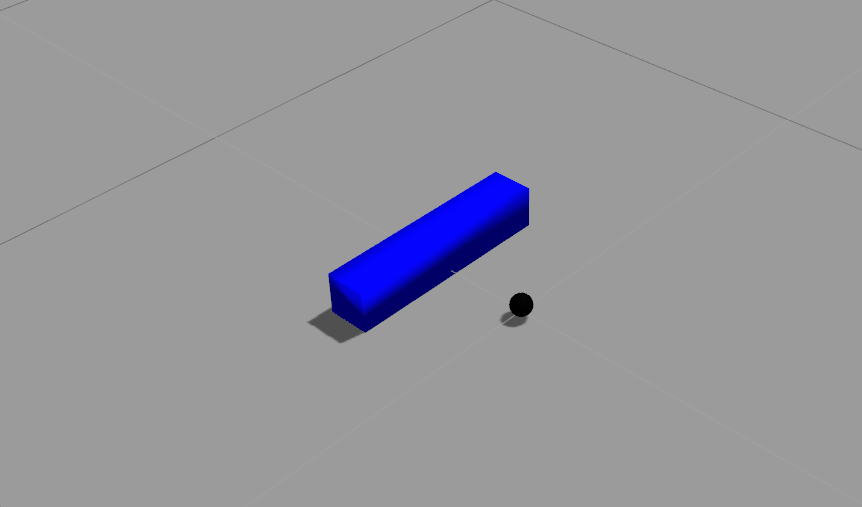
\includegraphics[width=10cm]{gazeboWorld.png} 
	\caption{Overview of the used environment. The black sphere represents the actuator, the models can control using action primitives. The blue square represents the object that the actuator interacts with.}
	\label{fig:gazeboWorld}
\end{figure}


\subsection{Communication}
Gazebo uses a client-server architecture. The actual simulation is being performed by the server.
This server publishes Google Protobuf \cite{protobuf} messages via TCP/IP. Interested clients, for example a graphical user interface, can register themselves as listener to messages of desired types. 
It is also possible to send messages to the server in order to influence the simulation. 

The server can furthermore be extended by writing custom plug-ins that handle self defined messages or perform some sort of additional computation at each update step of the simulation. 

In order for the Python prototypes to communicate with the simulation, an interface on both sides was created.

On the side of the simulation, a custom server plug-in was written. This plug-in publishes the information described in table \ref{tab:availInformation} in the realization chapter at the fixed rate. 
The information for all objects is packed into a custom Protobuf message, which is explained in details in Appendix \ref{sec:protobufMessages}. Basically, this message simply contains a list of object descriptions where each object description contains the information explained in table \ref{tab:availInformation}.
Furthermore, the plug-in receives custom control messages. These messages allow the Python interface to influence the simulation.
While the exact messages are explained in the Appendix \ref{sec:protobufMessages}, table \ref{tab:commands} gives an overview about the possible commands, that can be send to the simulation.

On the Python side, an interface was written with the help of the module pygazebo \cite{pygazebo}, which provides Python bindings for the message passing system used by gazebo. This interface handles the messages that are received from and send to the simulation. 
At each update step, the interface performs four to five actions:
\begin{enumerate}
\item Construct a suitable worldstate from the provided information
\item Get a prediction about the next worldstate from the model using the current worldstate
\item Update the model with the current worldstate
\item Get an action primitive from the model given a target configuration
\item Send the current action primitive to the simulation
\end{enumerate}

The 4th step is only performed in the tasks evaluating the inverse model. In the \textit{Push Task Simulation} a fixed action primitive is predetermined.

Furthermore, the Python interface provides the testing framework of setting up the models and managing training and testing runs as explained in detail below.

\begin{table}
	\centering
	\begin{tabular}{|c|c|}
		\hline \textbf{Command} & \textbf{Meaning} \\ 
		\hline Move Command & Sets the velocity for the actuator \\ 
		\hline Pause & Pauses the simulation \\
		\hline Continue & Continues the simulation \\
		\hline Reset & Resets all objects to starting configuration \\
		\hline Set Pose & Places a specified object at a certain position and orientation \\
		\hline
	\end{tabular} 
	\caption{Overview of all implemented commands to influence the simulation.}
	\label{tab:commands}
\end{table}

\subsection{Sources of noise}

Although the object's attributes can be read accurately from the simulation, some random noise is still present in the data: 

1) The physics simulation and the sensors that record the objects' attributes are run in different threads within the simulation. These threads cannot always be perfectly synchronized which can result in minor differences in consecutive timesteps. 

2) The physics simulation itself might encounter numerical instabilities, especially when computing resting forces. These instabilities
might lead to small oscillations within an object's features, such as position. In order to filter out such small noise, all
information from the simulation is rounded to 3 decimal places while constructing the worldstate. 

3) The strongest variation comes from the fact that the implementation communicates with the simulation via asynchronous messages. 
All runs start in a configuration where all objects are resting. In the very first update step, the Python interface sends the first
action primitive to the simulation, which results in the actuator moving. The exact time when the simulation retrieves and executes
the action is however not deterministic. Depending on the system's load the simulation might have already performed 5 update steps before
it receives and executes the action. In this case, the action affects only half of the update steps. In another situation, the action might
be executed earlier. From the model's point of view, the same action was performed from the same initial situation, but the resulting changes in object states can differ greatly. 

Since this thesis considers a rather simple scenario and these three sources of noise are already present due to the used technologies,
no additional artificial noise was introduced to the system. Both models needed to be flexible enough to learn from the noisy data without
fixating on outliers.

\section{Push Task Simulation \label{sec:pushTaskSim}}

The \textit{Push Task Simulation} is designed to test the accuracy of the forward model of both concepts. 

\subsection{Scenario description}

In this task, the actuator uses a constant action primitive in order to first move towards the block and then push it.
In order to evaluate different interactions, the actuator starts at different starting positions on a line parallel to the block. 

The distance between the starting line and the center block is 25cm. With the used speed, the actuator reaches the block in about 35 update steps after the start of a run. Depending on the third issue explained above, this number can vary a little.

After 150 update steps, a \textit{run} ends and the objects are reseted. This means, that the block will be placed at its resting position and the actuator is moved back to the starting line. 

During a run, the block status can change in a number of ways. In case the actuator goes past the block, it will not change at all. If it is pushed in the center, it will be translated up to \m{0.6}. Furthermore, depending on where the block is pushed, it will be rotated up to \rad{1.02} (around 58°) in either direction. The maximum rotation is experienced when the actuator starts around \m{0.105} away from the origin.

An example starting and end configuration can be seen in figure \ref{fig:pushTaskSim}. 

As the name suggest this task is designed to evaluate the prediction performance of the models during the pushing interaction. The \enquote{simulation} part of the name comes from the fact, that the models will make consecutive predictions based on their last prediction. At the start of each run, the models will make their first prediction based on the current worldstate provided by the simulation. This prediction is then used to construct an appropriate next worldstate which is used at the next update step from the simulation.
Furthermore, the predicted states of both the actuator and the object are send to the simulation for visualization as can be seen in figure \ref{fig:pushTaskSim}.

The models will not get any feedback from the real environment in this setting during testing, which means that they will not be able to adapt their predictions based on the actual interaction. 

In order to be able to make predictions at all, the model will first perform a number of training runs. During these training runs, the models are provided with the current worldstate from the simulation in order to train their local models.

In all runs, an action primitive is used that sets the velocity of the actuator to 0.5m/s straight upwards. Although only a constant global action is used, the prediction task is still challenging enough: \\
The constant action primitive does make it easy for the object state concept to learn the forward model of the actuator. However, the local forward model for the object is not as simple because the velocity is not constant in local coordinates but rather depends on the object's orientation. 
Similarly, in the interaction concept the used action primitive is also transformed to the local coordinate frame of the reference object.

Different kinds of training scenarios are evaluated in this task which are further explained below when their results are presented.


\begin{figure}
	\centering
	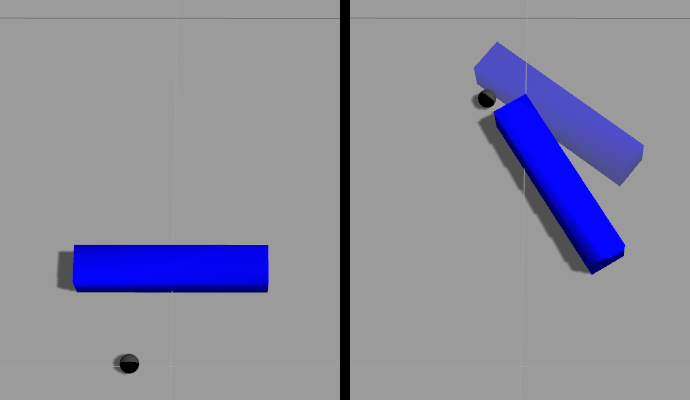
\includegraphics[width=0.8\textwidth]{PushTaskSim.png}
	\caption{Exemplary start and end configuration of a \textit{Push Task Simulation} run. The left side shows the start configuration, while on the right the corresponding end configuration can be seen.
		The darker objects (dark blue and black) represent the actual block and actuator, while the transparent objects symbolize the predicted objects.}
	\label{fig:pushTaskSim}
\end{figure}


\subsection{Evaluation criteria}

This task tries to evaluate the precision of the different models. In order to measure this precision, the distance between the predicted object state and the actual object state is computed at the end of each test run.
In this scenario, the models predict up to two quantities: The position and the orientation. 

As already mentioned before, finding a metric that can adequately combine differences in position and orientation at the same time is difficult. Furthermore, the interpretation of such a measurement is not intuitive. Therefore, the differences in position and orientation are considered separately. 
The positional difference is computed by the euclidean distance between the centers of the predicted and the actual object. The difference in orientation is given by the absolute difference between the predicted and the actual orientation.

Each training and testing setting is repeated 20 times and the average differences in position and orientation as well as their standard deviations are reported. 

\subsection{Evaluated configurations}
%TODO
The implementations of both concepts offer several possible configurations, beginning by using different features, to using hard coded components in the gating concept and choosing different learning rates for the underlying regression and classification models.

In this evaluation, the implementations are evaluated first in the configuration described in the last chapter with meta parameters chosen as indicated by table \ref{tab:parameters}

\begin{table}
	\centering
	\begin{tabular*}{\textwidth}{@{\extracolsep{\fill}} c c c }
			\hline \textbf{Parameter} & \textbf{Interaction} & \textbf{Gate} \\ 
			\hline \hline 
			 $\sigma$ & 0.05 & 0.05 \\
			 $\eta_{max}$ & 0.001 & 0.001 \\  
			\hline 
	\end{tabular*} 
	\caption{Table summarizing the meta parameters used for the presented evaluations.}
	\label{tab:parameters}
\end{table}

\subsection{Results}

\textbf{Generalization on random training data:}

%TODO if another object is added, specify which one is used here
The first test evaluates the prediction accuracy against the number of random training runs. The training run start positions were chosen at random in the range of \m{-0.25} to \m{0.25}. This means that they span the entire width of the block objects.
For each number of training runs that were evaluated, 21 test runs were performed with starting positions from \m{-0.35} to \m{0.35} at \m{0.035} intervals. This means that 6 test runs went past the object without interacting with it.
The averaged results for the block predictions over all folds for the interaction state model in the first configuration can be seen in figure \ref{fig:learnCurveInteraction1}. The averages over all test runs as well as only over the 15 central test positions are shown.

\begin{figure}[h]
\centering
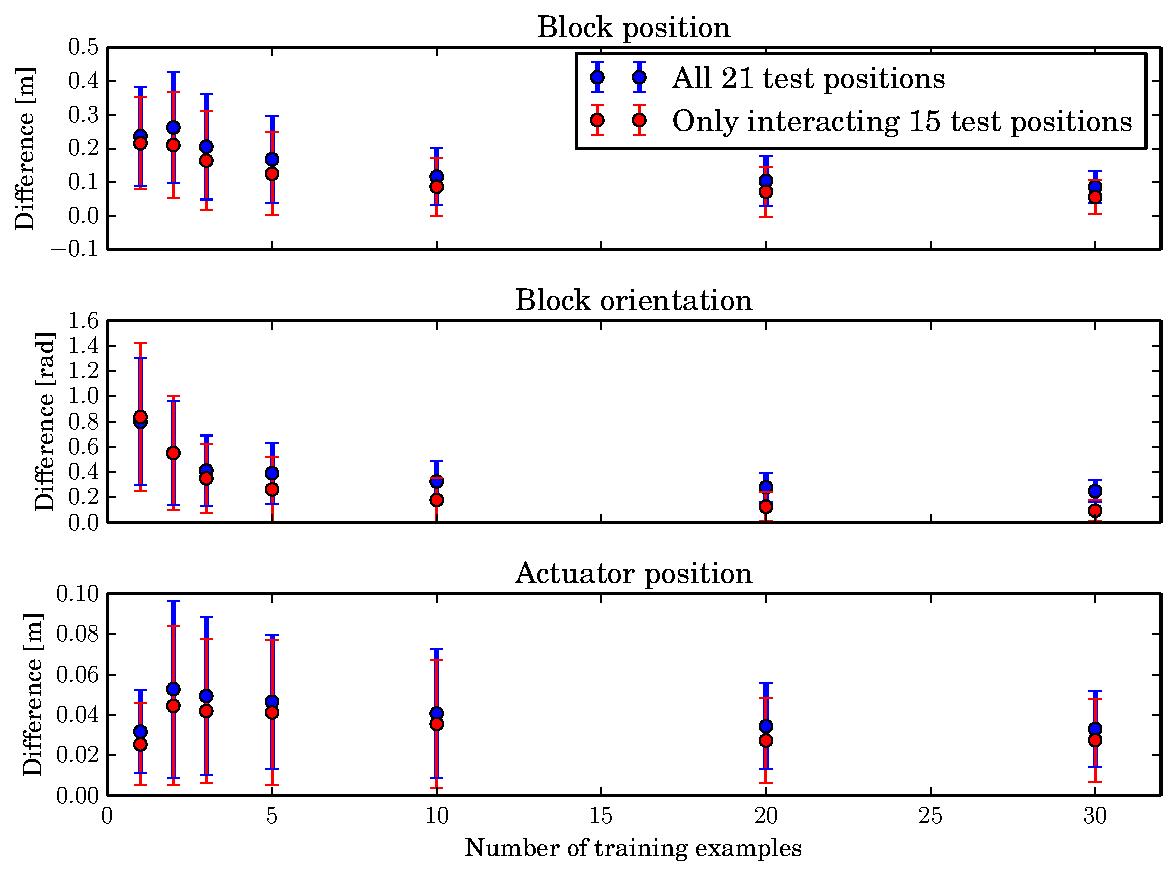
\includegraphics[width=0.7\textwidth]{LearningCurveinteractionModel_C_0E20FoldsSigma005.pdf}
\caption{Learning curve for the interaction concept in the first configuration. Difference in position and orientation for the block predictions and differences for the actuator position at the end of a run are shown. Error bars indicate one standard deviation. Blue error bars represents averages over all 21 test positions, while red error bars only averages over the 15 test positions where the block is actually moved.}
\label{fig:learnCurveInteraction1}
\end{figure}

The positional prediction error starts around \m{0.24} with a standard deviation of around \m{0.15} when the model is only trained with a single training example. The prediction performance improves to roughly \m{0.09} with a standard deviation of around \m{0.05}.
The predicted orientation error starts at an average of about \rad{0.8} with standard deviation of \rad{0.5} but improves to around \rad{0.25} with standard deviation of \rad{0.09} when increasing the number of random training examples.
The performances for position and orientation do not increase much more after the first 10 training runs (\m{0.12} $+/-$ \m{0.08} for position and \rad{0.33} $+/-$ \rad{0.16} for orientation).
The actuator position predictions remain fairly constant with errors around \m{0.03} with a standard deviation of \m{0.02} for all training scenarios.

When only considering the testing positions where the actuator actually interacts with the block (red error bars), predicted errors improve slightly.

The results for the same experiment with the object state with gating function model using the first configuration are presented in figure \ref{fig:learnCurveGate1}.

\begin{figure}[h]
\centering
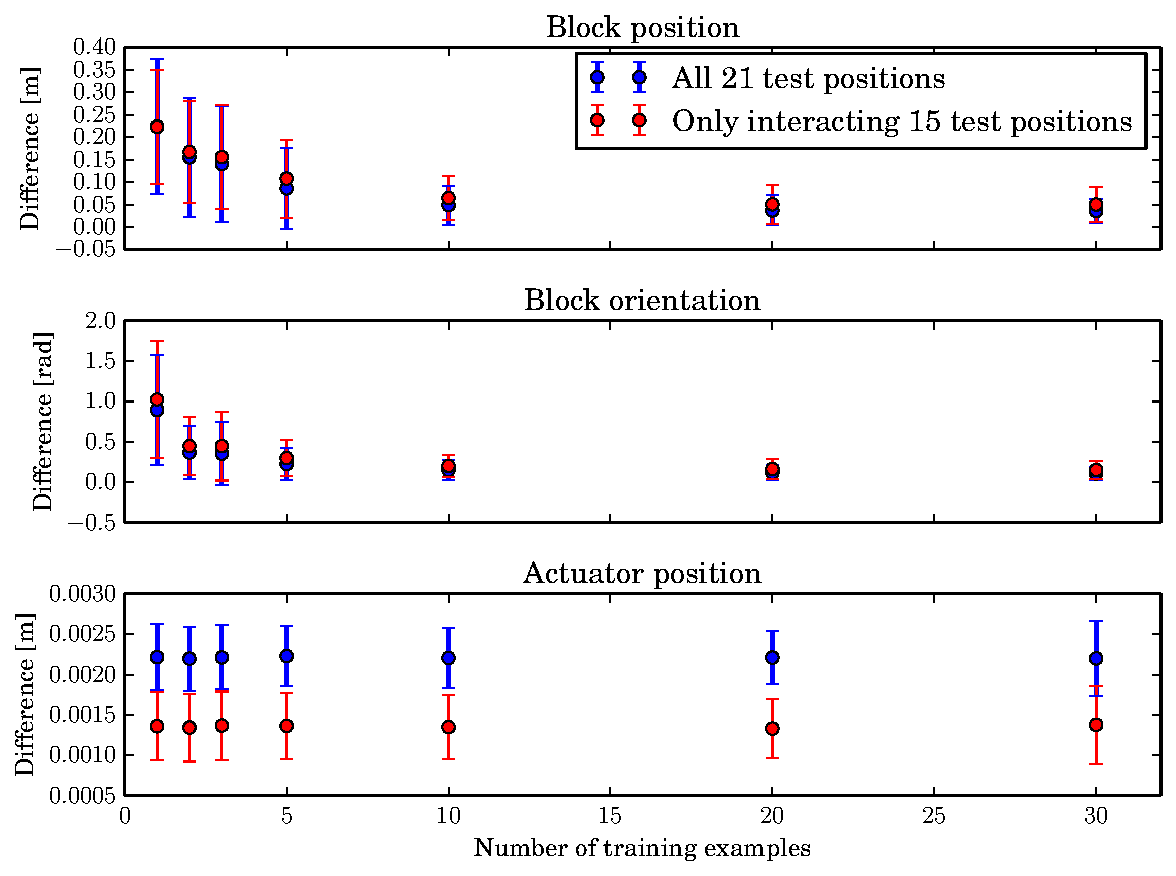
\includegraphics[width=0.7\textwidth]{LearningCurvegateModel_C_0E20FoldsAllGateFSigma005.pdf}
\caption{Learning curve for the object state with gating function concept. Difference in position and orientation for the block predictions and differences for the actuator position at the end of a run are shown. Error bars indicate one standard deviation. Blue error bars represents averages over all 21 test positions, while red error bars only averages over the 15 test positions where the block is actually moved.}
\label{fig:learnCurveGate1}
\end{figure}

The positional prediction error over all testing positions (blue error bars) starts at around \m{0.22} with a standard deviation of \m{0.15} for only one training run in the object state with gating function model. By increasing the number of random training runs to 30, the positional error reduces continuously to around \m{0.04} with standard deviation of only around \m{0.03}.
The predicted orientation error starts at around \rad{0.89} with standard deviation of \rad{0.68}.
After 30 test runs an error of \rad{0.10} with a standard deviation of \rad{0.08} remains.
For this model the performance increases only slightly with more training runs after having seen only 10 training runs for both the error in position (\m{0.05} $+/-$ \m{0.04}) as well as orientation (\rad{0.18} $+/-$ \rad{0.12}).
Predictions for the actuator position are fairly constant around \m{0.002} with a standard deviation of around \m{0.0004}.

Unlike in the other model, prediction errors are slightly worse for the block position and orientation when only considering the 15 testing positions where an actual interaction takes place. Actuator prediction are slightly more accurate however.

Memory-based regression methods such as \gls{nn} approaches often suffer from the increasing computational complexity as the number of training samples increases.
Table \ref{tab:learnCurveGateNodes} shows the average number of update calls and number of nodes in the \glspl{aitm} used by the object state model after training for the different number of training runs. Similarly, table \ref{tab:learnCurveInteractionNodes} presents similar numbers for the interaction state model. Since the number of learned \glspl{ac} varies between the runs, only the number of nodes for the \gls{ac} with the most nodes is recorded. 
Only 149 update calls are made at most for each run because the models are not updated after the 150th timestep.


\begin{table}
\footnotesize 
	\centering
	\begin{tabular*}{\textwidth}{@{\extracolsep{\fill}} c c c c c}
			\hline \textbf{Train runs} & \textbf{Object Updates}&  \textbf{Object Nodes} & \textbf{Gate Updates} &\textbf{Gate Nodes} \\ 
			\hline \hline 
			 1 & 93.5 & 26.55 & 149 & 3.7 \\
			 2 & 194.35 & 39.4 & 298 & 5.55 \\  
			 3 & 287.25 & 67.4 & 447 & 6.4 \\
			 5 & 479.6 & 111.95 & 745 & 6.8 \\
			 10 & 963.7 & 219.65 & 1490 & 7.75 \\
			 20 & 1894.25 & 438.2 & 2980 & 10.4 \\
			 30 & 2883.8 & 603.05 & 4470 & 10.2 \\
			\hline 
	\end{tabular*} 
	\caption{Record of the average number of nodes that resulted from the recorded number of update calls in the regression and classification \gls{aitm} for the object state model.}
	\label{tab:learnCurveGateNodes}
\end{table}

Interestingly, the number of nodes required for the gating function is rather constant whereas the local forward model in the predictor creates a node between every 4th and 5th update call on average. 

\begin{table}
\footnotesize 
	\centering
	\begin{tabular*}{\textwidth}{@{\extracolsep{\fill}} c c c c c}
			\hline \textbf{Train runs} & \textbf{AC Updates}&  \textbf{AC Nodes} & \textbf{ACS Updates} &\textbf{ACS Nodes} \\ 
			\hline \hline 
			 1 & 93.5 & 26.55 & 149 & 3.7 \\
			 2 & 194.35 & 39.4 & 298 & 5.55 \\  
			 3 & 287.25 & 67.4 & 447 & 6.4 \\
			 5 & 479.6 & 111.95 & 745 & 6.8 \\
			 10 & 963.7 & 219.65 & 1490 & 7.75 \\
			 20 & 1894.25 & 438.2 & 2980 & 10.4 \\
			 30 & 2883.8 & 603.05 & 4470 & 10.2 \\
			\hline 
	\end{tabular*} 
	\caption{Record of the average number of nodes that resulted from the recorded number of update calls in the regression and classification \gls{aitm} for the interaction model. Only the number of the \gls{ac} with the most nodes is recorded.}
	\label{tab:learnCurveInteractionNodes}
\end{table}

\textbf{Generalization on selected training data:}

In order to analyze the information required for generalization, another training scheme was used. This time the models were only provided with three predetermined training runs. The starting positions \m{-0.18}, \m{0.0} and \m{0.18} were used in this experiment. These three were chosen in order to provide the models with examples of both possible rotations as well as the lateral movement. The same 21 test runs were performed as before. This time prediction errors at the end of the run are recorded for each starting position separately. Due to the noise explained above, some randomness is still present in the data which is why this experiment was also repeated 20 times and the average errors are reported. 

The results for the interaction model are shown in figure \ref{fig:eachPosInteraction}.

\begin{figure}
\centering
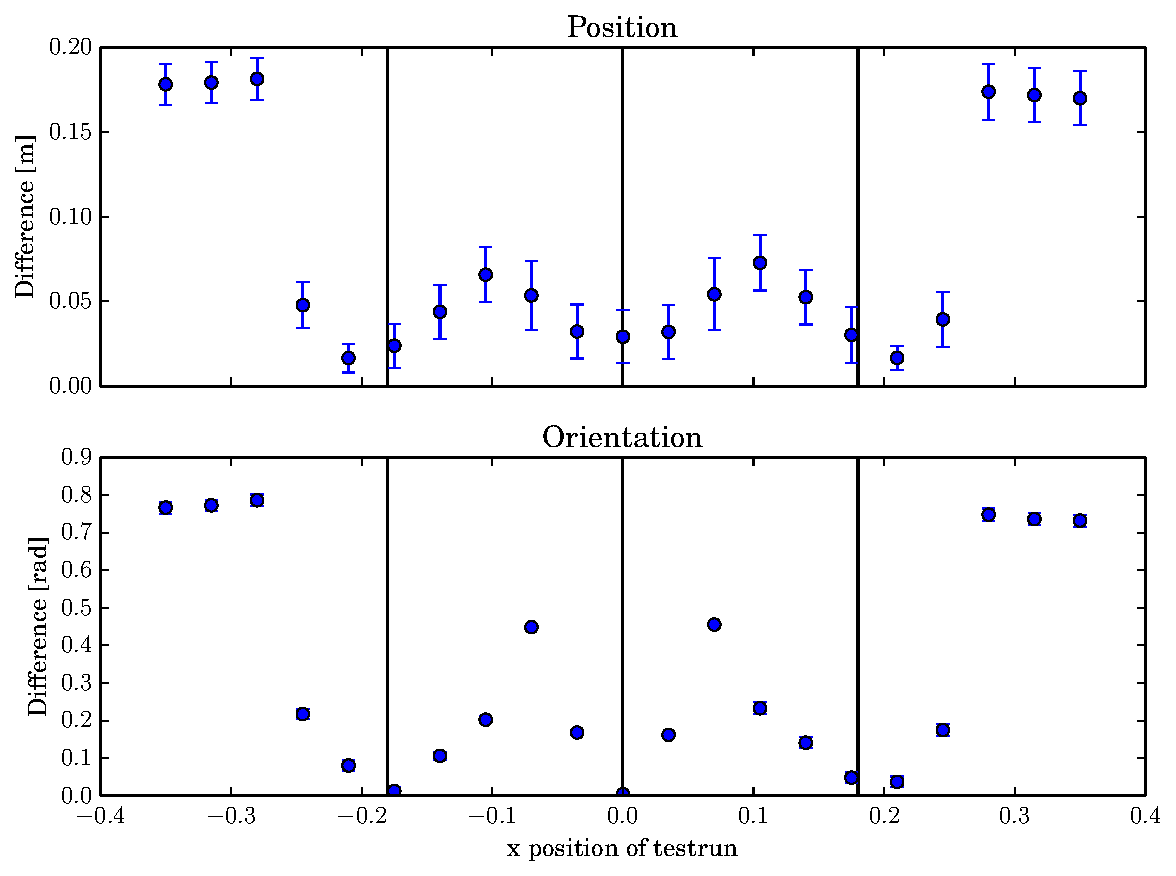
\includegraphics[width=0.7\textwidth]{EachPositioninteractionModel_C_8E20FoldsAllACSFSigma005.pdf}
\caption{Prediction errors for the interaction model at each of the 21 test positions after seeing three exemplary training examples. The training positions are highlighted by the block lines. Error bars indicate one standard deviation.}
\label{fig:eachPosInteraction}
\end{figure}

As mentioned in the previous setting, the predictions for the test runs that do not actually interact with the block, are rather poor. The model predicts an incorrect change in position around \m{0.18} +/- \m{0.01} and in orientation around \rad{0.77} +/- \rad{0.02} on both sides of the object. 
Predictions are quite good close to the seen training examples when the block is actually influenced: The positional error is as low as \m{0.02} +/- \m{0.01} around the two outer training positions and slightly higher for the central position (\m{0.03} +/- \m{0.02}). Generally the same applies for orientation, but the central position has a prediction error for orientation of around 0, while the outer positions are slightly higher (\rad{0.01} +/- \rad{0.01}).
The further away from the training positions, the worse the prediction for both position and orientation becomes. Interestingly, the worst positional prediction of \m{0.07} +/- \m{0.02}  happens \m{0.105} away from the center, while the worst prediction for orientation of \rad{0.45} +/- \rad{0.01} is seen \m{0.07} away from the center.

It is also interesting to note, that the position and orientation are predicted very consistently (most standard deviations below \m{0.02} and all below \rad{0.02}).

The results for the same experiment performed with the object state model are presented in figure \ref{fig:eachPosGate}.

\begin{figure}
\centering
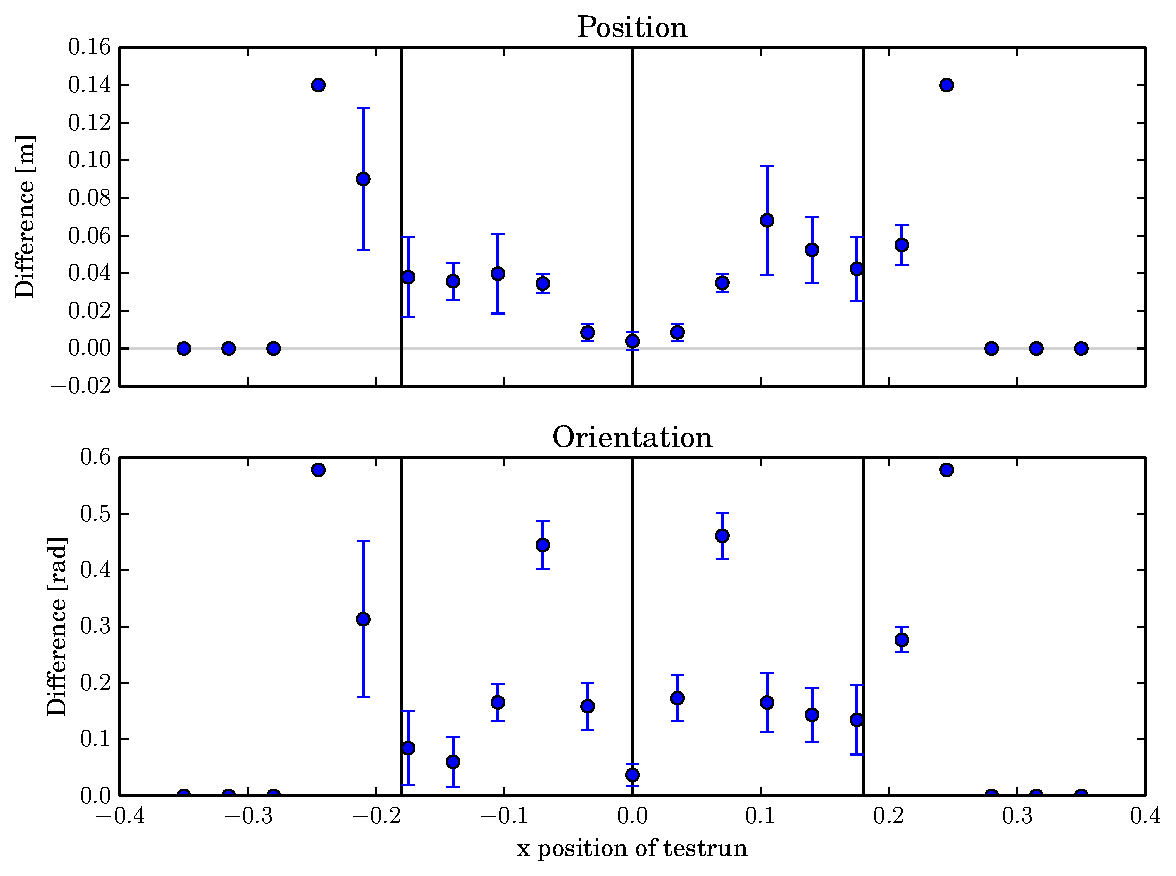
\includegraphics[width=0.7\textwidth]{EachPositiongateModel_C_8E20FoldsAllGateFSigma005.pdf}
\caption{Prediction errors for the object state model at each of the 21 test positions after seeing three exemplary training examples. The training positions are highlighted by the block lines. Error bars indicate one standard deviation.}
\label{fig:eachPosGate}
\end{figure}

The object state with gating function successfully does not make predictions for the test runs that go past the object after seeing the three fixed training runs. However, no predictions are also made for the first interacting test positions on either side which results in constant errors in position of \m{0.14} and in orientation of \rad{0.58}.
For the other test positions that actually interact with the block, the predictions are better for positions close to the training examples as in the other model.
The predicted errors are not quite as symmetric as in the other model.
The central position has a prediction error of close to 0 with a standard deviation below \m{0.01}. 
The predictions for position are slightly more accurate between the left and the middle training position (ranging from \m{0.01} +/- \m{0.0} to \m{0.04} +/- \m{0.02}) when compared to the testing positions between the middle and the right training position (ranging from \m{0.01} +/- \m{0.0} to \m{0.07} +/- \m{0.03}). Outside the training positions, the predictions are better for the 17th testing position than for the fifth one (\m{0.09} +/- \m{0.04} at the fifth and \m{0.06} +/- \m{0.01} at the 17th testing position).

Prediction errors for orientation show a similar trend: 
In the central position the prediction error in orientation is \rad{0.04} +/- \rad{0.02}.
The same outliers for orientation are found as in the other model. The testing positions \m{0.07} away from the center have errors around \rad{0.45} +/- \rad{0.04}
The remaining errors for orientation in between the training positions are ranging from \rad{0.06} +/- \rad{0.04} to \rad{0.16} +/- \rad{0.05}.
As with the positional prediction, the prediction for orientation is slightly worse for the fifth testing position compared to the 17th one, although both have the same distance to the closest training position (\rad{0.31} +/- \rad{0.14} at the fifth and \rad{0.28} +/- \rad{0.02} at the 17th testing position).

In order to be able to interpret these results, figure \ref{fig:EachPosEndPos} shows a final configurations (predicted and actual) for every 2nd testing positions for both models.

\begin{figure}
\centering
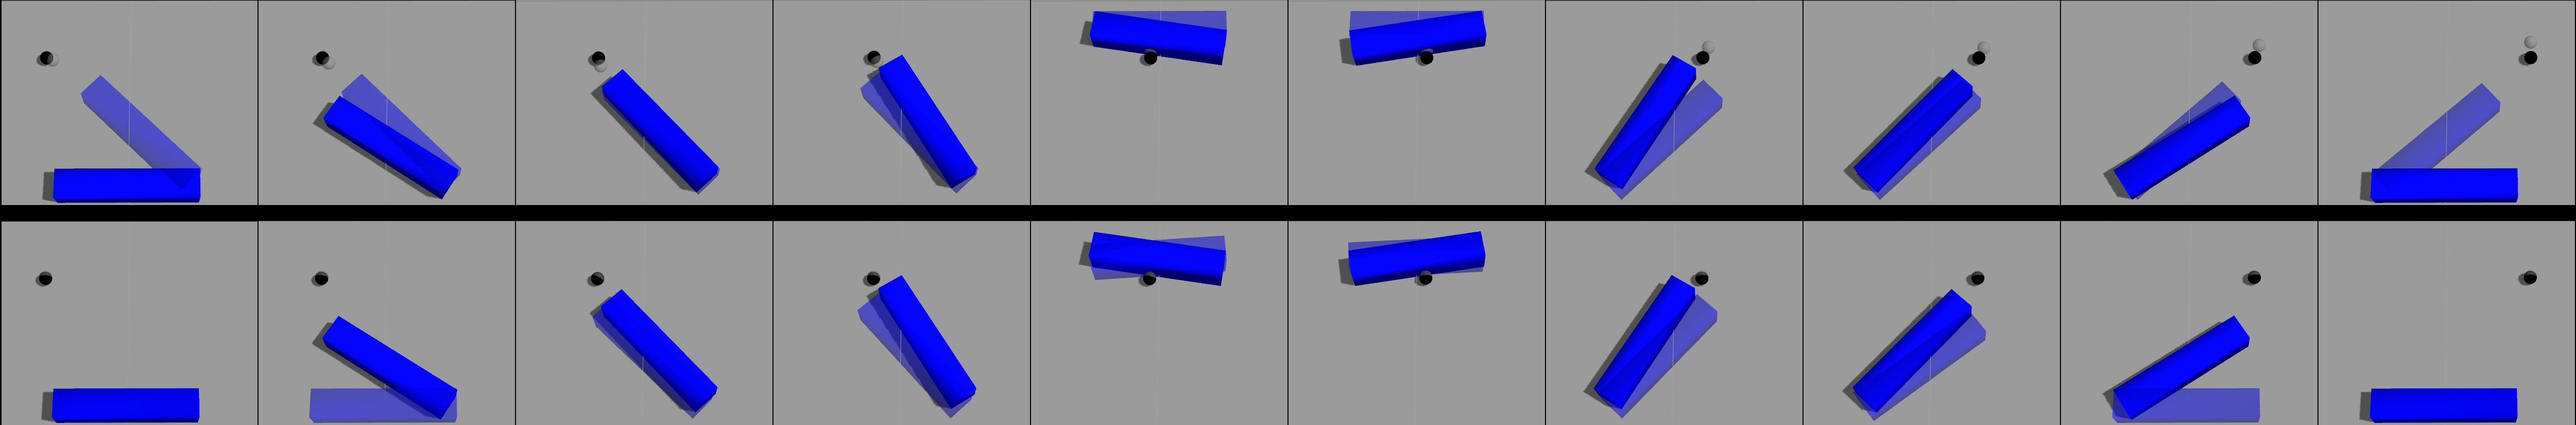
\includegraphics[width=\textwidth]{EachPosEndPos.png}
\caption{Predicted and actual end positions. Transparent objects represent the predictions. Top row shows results for the interaction model, while bottom row shows the results for the object state with gating function model. Every 2nd of the 21 testing positions is shown. The training positions are right next to the third image on either side as well as between the two central images.}
\label{fig:EachPosEndPos}
\end{figure}

\textbf{Generalization in the open loop:}

While the previous scenarios test the accumulated prediction error, it is often not required to make accurate predictions 150 steps into the future. Instead it is more important to adapt to changes in the environment quickly. For that reason, a variation of the \textit{Push Task Simulation} was also evaluated. In this variation, the models are not trained before testing, but will instead continuously receive updates from the environment. That way the models online learning capabilities are evaluated. The models will still make consecutive predictions based on their last prediction. Their last predictions are not corrected based on the actual environment and the models do not get or compute any feedback as to how good their last prediction was. 

A qualitative evaluation is provided in figure \ref{fig:pushTaskSim2}. The figure shows images of consecutive interactions of the object state model with the environment. The transparent object represent the last predictions, while the darker objects represent the actual states of the objects. In order to be able to actually see meaningful differences between consecutive interactions, these images where taken in a setting where the model is only updated every 10Hz, meaning that the model was updated and queried every 0.1 seconds in simulation time instead of the 0.01 seconds used for all the other evaluations. No other adaptation to the model was made. The top row shows the first run the model performs while the second row shows the following run. The testing positions were predefined.

\begin{figure}
\centering
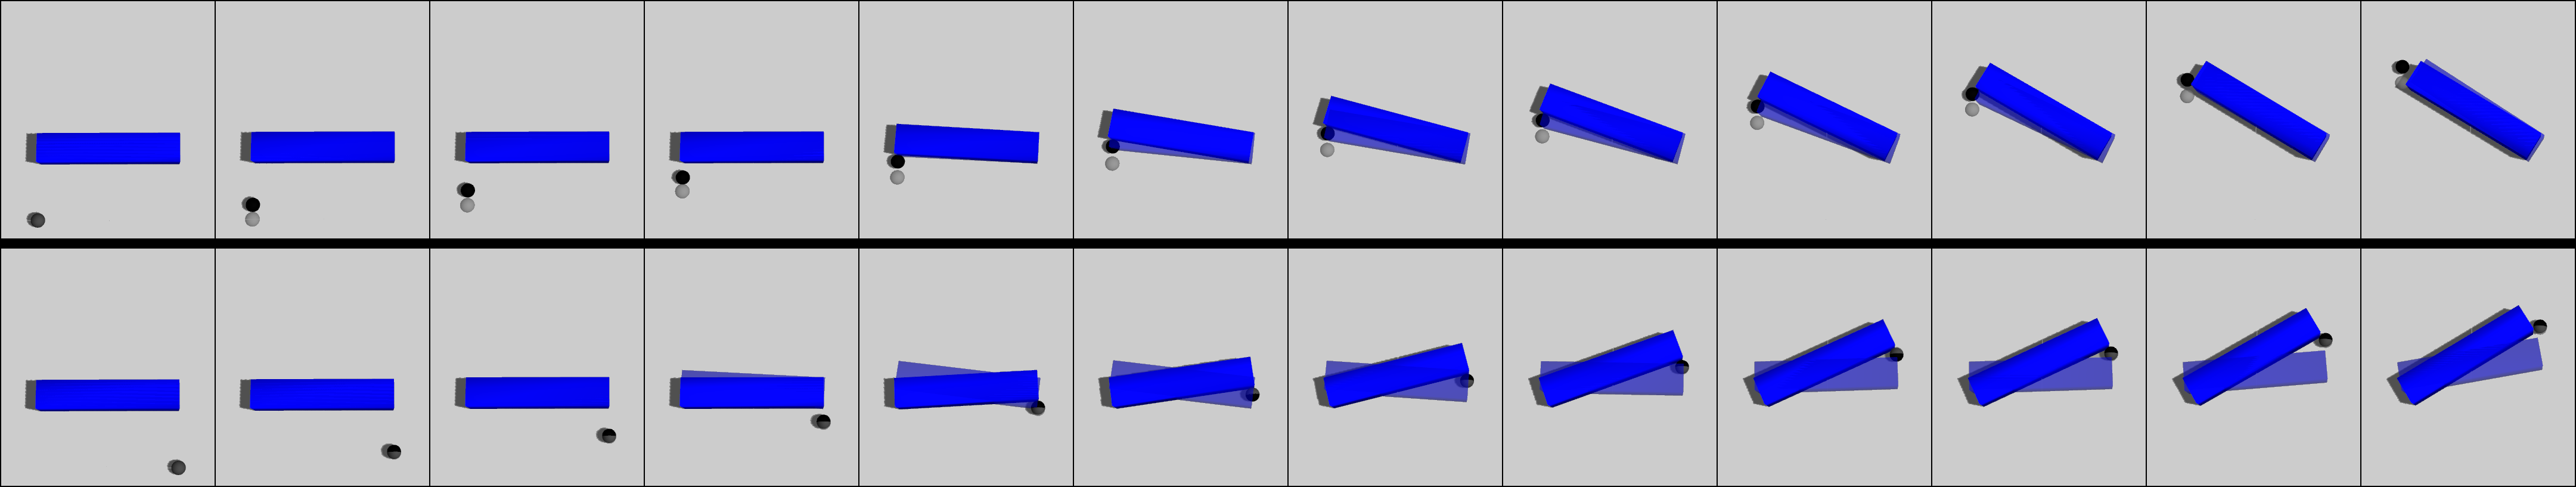
\includegraphics[width=\textwidth]{pushTaskSim2.png}
\caption{Consecutive interactions in the \textit{Push Task Simulation} variation. Top row shows images of the first test run, while the second row shows images of the second test run on the other side of the object. }
\label{fig:pushTaskSim2}
\end{figure}

The leftmost images show the initial configuration at the start of both runs. While no prediction is made for the actuator in the 2nd image of the top row, the actuator is predicted correctly in the 2nd run. The top row continues to lag one frame behind with its predictions. The final block predictions are accurate again.
In the 2nd run, the actuator predictions are good. However, the model predicts the same rotation as in the first run once the actuator comes close to the object. After a few other frames, the predictions start turning in the other direction, but do not catch up to the actual objects.


\subsection{Extension to multiple objects \label{sec:multipleObjects}}

Environments rarely only contain a single object, however, so far in this thesis, only one object was considered. While it is difficult for the interaction model to handle multiple objects due to the reasons explained in section \ref{sec:interactionTheory}, the object state model handles objects separately anyways. In this evaluation the red block described in table \ref{tab:environmentObjects} is added to the scene and six fixed (three interacting with each object) training positions are used. 
A fixed set of 21 testing positions ranging from \m{-0.8} to \m{0.4} in intervals of \m{0.06}.

The model was not altered in any way for the results presented in figure \ref{fig:eachPosTwoObjects}.

\begin{figure}
\centering
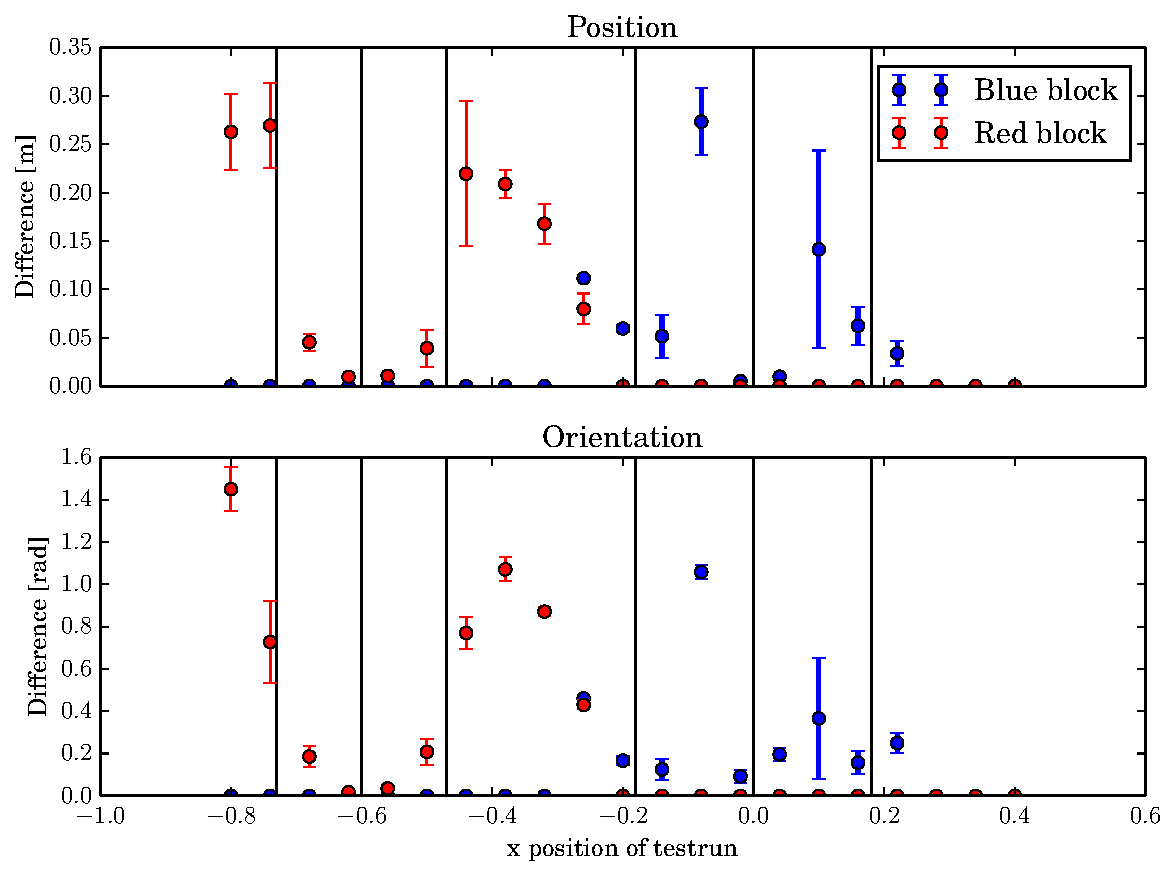
\includegraphics[width=0.7\textwidth]{EachPosgateModel_C_8E2ObjectsV2.pdf}
\caption{Prediction errors for the object state model with two objects. The training positions are highlighted by the black lines. Error bars indicate one standard deviation.}
\label{fig:eachPosTwoObjects}
\end{figure}

The gating function often classifies incorrectly for the red object, but the blue object does not seem to be influenced by the new object at all since the results are basically identical to the ones presented in \ref{fig:eachPosGate}.

By introducing a seventh training position in between both objects, improves the prediction quality due to better performance of the gating function as can be seen in figure \ref{fig:eachPosTwoObjects7Trains}.


\begin{figure}
\centering
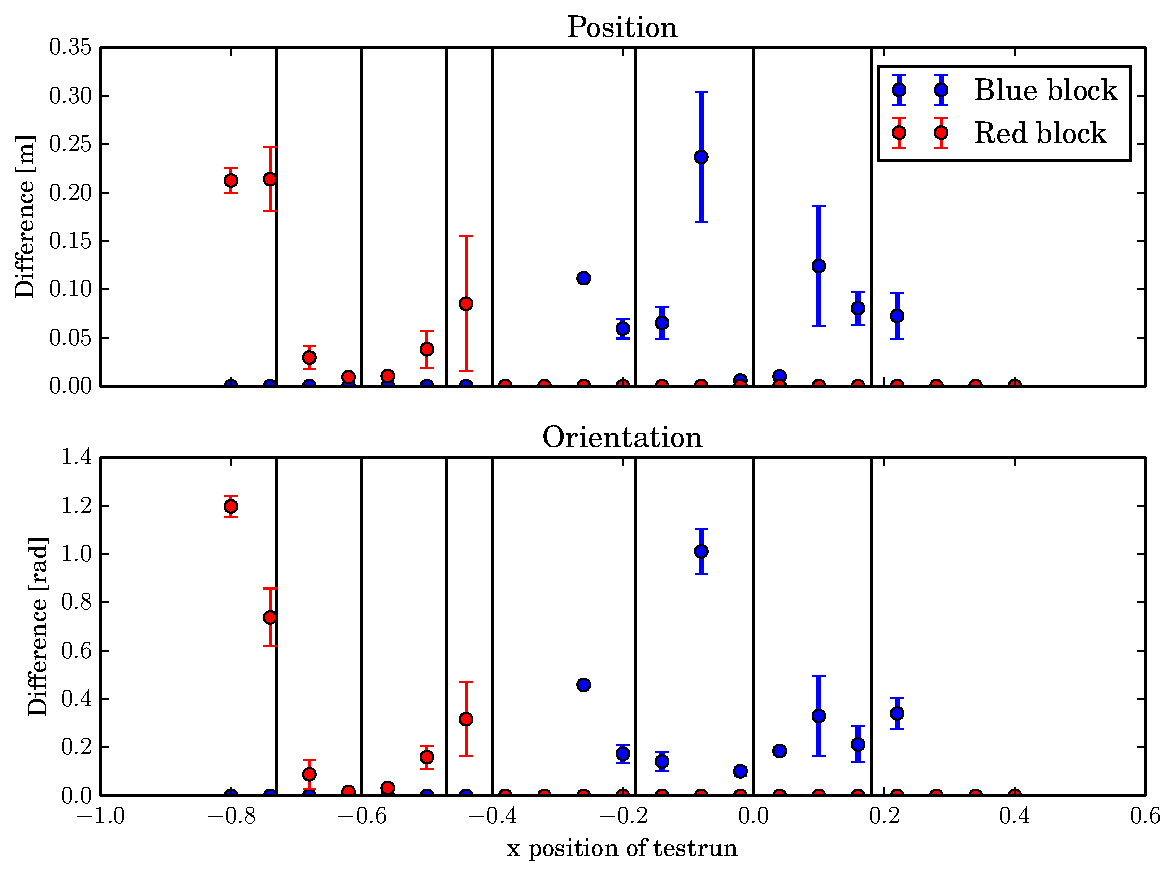
\includegraphics[width=0.7\textwidth]{EachPosgateModel_C_8E20Folds2Objects7Train.pdf}
\caption{Prediction errors for the object state model with two objects with an additional separating training positions. The training positions are highlighted by the black lines. Error bars indicate one standard deviation.}
\label{fig:eachPosTwoObjects7Trains}
\end{figure}


\section{Move to Target \label{sec:moveToTarget}}

The \textit{Move to Target} task is designed to evaluate the concept's ability to reach a given target configuration incrementally. 

\subsection{Scenario description}

In this task only a target configuration for the block object is given to the models. At each update step the models are updated with the current worldstate.
This means that they can adapt their inverse model during testing.
Afterwards, the interface queries the model for the next action primitive which is then send to the simulation. This is repeated until the target configuration is reached or a maximum number of steps of 3000 has been performed.
The models consider a target configuration as reached, if the norm of the difference vector between the target representation and the current situation is smaller than 0.01. This means, that the combined vector of positional difference as well as difference of orientation must have a norm smaller 0.01. The models do not know about the oscillation of the orientation feature, i.e. that an orientation of $-\pi = \pi$ which can lead to false negatives.

The models are first trained on a fixed set of training runs. The set is designed to show important interactions to the models before testing.

The training runs are performed by placing the actuator in a suitable starting position before applying a constant action primitive directed towards the block.
The used action primitives all have a norm of 0.5m/s.

After training, both the actuator and the block are returned to their initial position. The block is located \m{0.25} above the global origin without any rotation, while the actuator is placed directly on top of the global origin.
Figure \ref{fig:moveToTargetScenario} visualizes the situation where the actuator just starts moving after training. The transparent light blue block symbolizes the target configuration of the block.

\begin{figure}
\centering
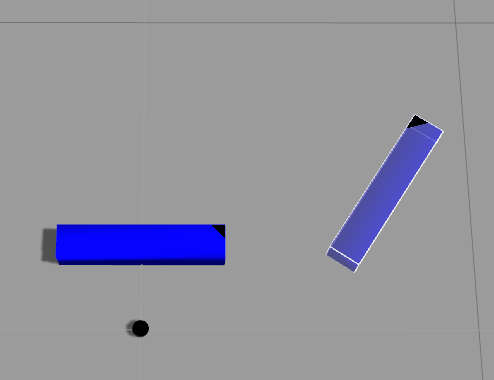
\includegraphics[width=0.5\textwidth]{MoveToTargetScenario.png}
\caption{Visualization of the \textit{Move to Target} task after training. The transparent light blue block indicates the desired target configuration. The blocks have been marked with the black corner to distinguish their orientation.}
\label{fig:moveToTargetScenario}
\end{figure}

\subsection{Evaluation criteria}

The performance of the inverse model is measured by the number of actions required to reach the target. If the target has not been reached within the allowed number of steps, the remaining difference is recorded. Similar to the previous task, position and orientation differences are recorded separately.

While recording the number of required steps, actual interactions where the block is moved and steps where only the actuator moves are distinguished.

Furthermore, the average change in position and orientation per performed action is reported in order to judge the quality of the selected action primitives.

The models are tested with four targets, each translated the same distance from the starting position but with different orientations. Figure \ref{fig:targetPositions} shows the four different target configurations. All target configurations have the same positional difference to the starting position (\m{0.6} in either x direction and \m{0.7} in either y direction) but different orientations: 
\begin{itemize}
\item Target 1: \rad{-2.1}
\item Target 2: \rad{0.75}
\item Target 3: \rad{0.0} 
\item Target 4: \rad{3.1415}
\end{itemize}
For each target, the model is trained separately on the same training set in order to ensure comparability between the targets.

The testing of each target configuration is repeated 5 times and the averages over these runs are reported where possible.

\begin{figure}
\centering
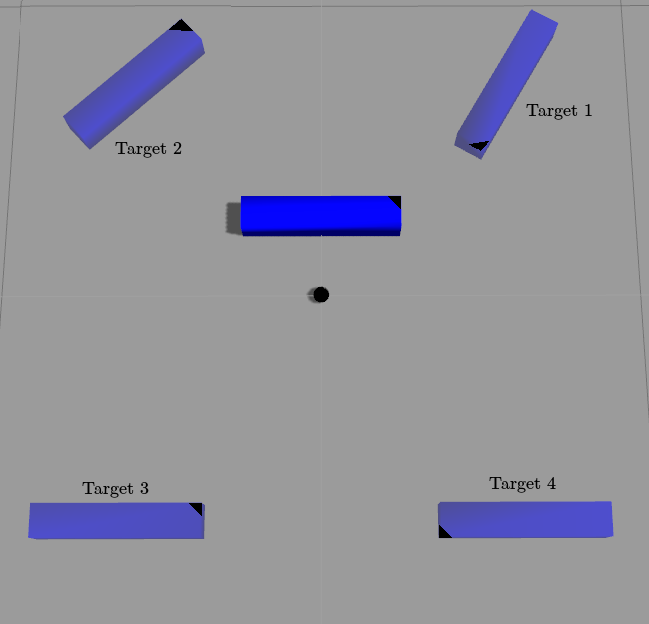
\includegraphics[width=0.5\textwidth]{MoveToTargetTargets.png}
\caption{Visualization of the four target configurations for the \textit{Move to Target} task. The black corners indicate the block's rotation.}
\label{fig:targetPositions}
\end{figure}

\subsection{Results}
The models were first evaluated after seeing the eight training runs visualized in figure \ref{fig:moveToTargetTraining}. These training runs ensure that the inverse models can learn reasonable preconditions for all relevant feature changes.

\begin{figure}
\centering
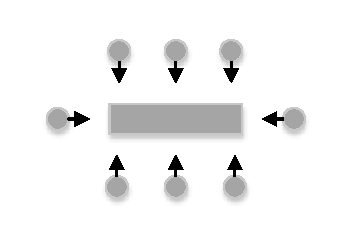
\includegraphics[width=0.5\textwidth]{MoveToTargetTraining.pdf}
\caption{Visualization of the eight training positions for the \textit{Move to Target} task. The circles indicate the relative starting positions of the actuator, while the arrows indicate the used action primitive.}
\label{fig:moveToTargetTraining}
\end{figure}

The results for the interaction models are presented in table \ref{tab:moveToTargetInteractionResults} while the results for the object state with gating function model are presented in table \ref{tab:moveToTargetGateResults}.

\begin{table} %USE V2 sigma 0.05
	\centering
	\begin{tabular*}{\textwidth}{@{\extracolsep{\fill}} c c c c c } %c c}
			\hline \textbf{Target} & \textbf{Reached} & \textbf{Pos} & \textbf{Ori} & \textbf{\# steps} \\%& \textbf{Avg pos} & \textbf{Avg ori} \\ 
			\hline \hline 
			 Target 1 & 3 & 0.55 & 0.002 & 2689.2 (2482) \\ %&  & \\
			 Target 2 & 4 & 0.01 & 0.023 & 2430.4 (2288) \\ %& &  \\  
			 Target 3 & 5 & - & - & 1377.6 \\ %& &  \\  
			 Target 4 & 2 & 0.55 & 2.04 & 2492.2 (1730.5) \\ %& &  \\  
			\hline 
	\end{tabular*} 
	\caption{Evaluation results for the \textit{Move to Target} task for the interaction model. Pos and Ori columns represent the remaining error in position ([m]) and orientation [rad] respectively for the runs that did not reach the target. The number of steps in brackets represents the average over the runs that reached the target.}
	\label{tab:moveToTargetInteractionResults}
\end{table}

The object state with gating function reaches the targets in most cases within the allowed number of steps. 
%TODO redo with hopefully decent data ...
No target is never reached, but the interaction model had a few problems reaching the first and fourth targets. Looking at the combined error of position and orientation for the 3 runs that did not reach the Target 4 in figure \ref{fig:moveToTargetInteractionT4Detail} reveals, that 2 of these runs were actually quite close to the target.

Target 1 appears to be more difficult for the object state model as the average number of steps is significantly higher then for the other target configurations.


\begin{figure}
\centering
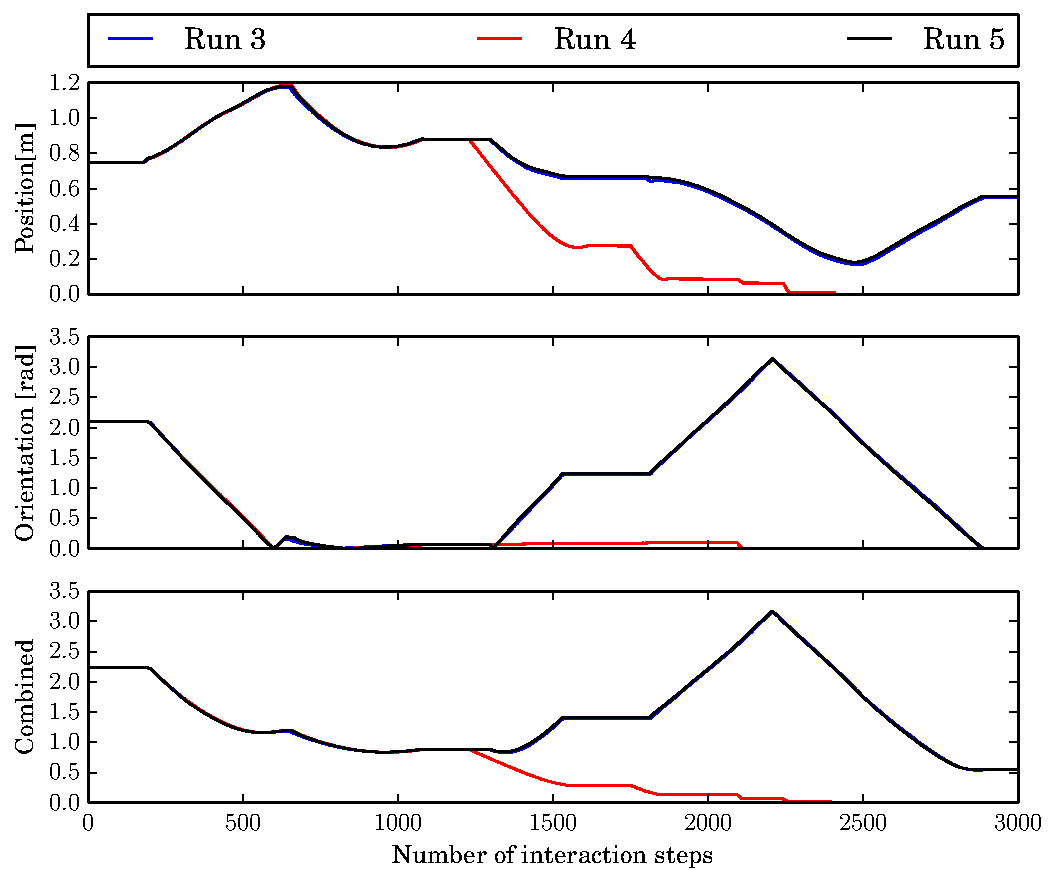
\includegraphics[width=0.8\textwidth]{MoveToTargetInteractionT1Detail.pdf}
\caption{Detailed view of the three runs towards Target 1 that did not reach the target in the interaction model. The errors in position and orientation as well as the combined error over the interaction steps are shown.}
\label{fig:moveToTargetInteractionT1Detail}
\end{figure}

The marked run for Target 4 in the interaction model is shown in greater detail in figure \ref{fig:moveToTargetInteractionT4Detail}. According to the combined error, the target was reached after around 1500 steps, but the model did not detect that and moved the block away from the target position again.
\begin{table}
	\centering
	\begin{tabular*}{\textwidth}{@{\extracolsep{\fill}} c c c c c } %c c}
			\hline \textbf{Target} & \textbf{Reached} & \textbf{Pos} & \textbf{Ori} & \textbf{\# steps} \\ %&  \textbf{Avg pos} & \textbf{Avg ori} \\ 
			\hline \hline 
			 Target 1 & 4 & 0.01 & 0.002 & 2271 (2088.8) \\ %& & \\
			 Target 2 & 5 & - & - & 1695 \\ %& &  \\  
			 Target 3 & 5 & - & - & 1147.4 \\ %& &  \\  
			 Target 4 & 5 & - & - & 1597.4 \\ %& &  \\  
			\hline 
	\end{tabular*} 
	\caption{Evaluation results for the \textit{Move to Target} task for the gate model. Pos and Ori columns represent the remaining error in position ([m]) and orientation [rad] respectively for the runs that did not reach the target. The number of steps in brackets represents the average over the runs that reached the target.}
	\label{tab:moveToTargetGateResults}
\end{table}





  \chapter{Discussion \label{chap:discussion}}

%TODO text here??
\section{Generalization performance}

The first task was designed to evaluate the generalization capabilities of the memory based concepts. It is important to note, that no domain knowledge outside the stated assumptions was provided to either model for this prediction task. Although the used features were selected by hand, no preprocessing of these features is performed and no knowledge about special feature dimensions is provided. It is highly likely, that the generalization performance of both models could be increased by providing fine tuned distance metrics and/or preprocessing the used features.
However, such knowledge is usually not available to the machine when encountering novel situations which is why such optimizations were not considered here.

\subsection{Generalization on random training data}

Prediction performances of both models reach acceptable levels for position and orientation considering 150 timesteps are predicted without correction. 
Both models prediction for the blocks position are on average less then 10cm incorrect after having seen 30 random training runs. The models predict the rotation of the objects correct up to an average error of around 15° for the interaction, and less then 6° for the object state model.

Overall, the object state model outperforms the interaction state model by requiring less training runs while achieving better prediction results as soon as at least 2 training runs have been seen.
%This holds true for both tested configurations as can be seen when comparing figures \ref{fig:learnCurveGate1} and \ref{fig:learnCurveInteraction1}. 
%TODO check if really for both configurations
This performance difference is most likely due to the higher complexity of the Abstract Case Selector compared to the gating function. While the gating function only needs to learn a binary classifier, the Abstract Case Selector, needs to choose from a potentially big number of possible local models. Choosing an incorrect model results in a poor prediction, which will be accumulated over the course of the test run. Furthermore, the gating function is provided with more information than the Abstract Case Selector, due to the features distance and closing, that are introduced in the relative interaction features. 

The better performance of the interaction model after just one training run, is most likely due to the fact, that the gating function needs at least two runs before it works sufficiently well. If the gating function performs poorly, an incorrect choice by the Abstract Case Selector might still result in a better prediction than predicting no change at all.
%In fact these two features are sufficient for the gating function to learn when the actuator influences the block as can be seen by the better results of the second configuration. 
%Since the local forward model for the object group is trained in the same way as in the other configuration, the better overall performance can only be due to the selected features.

%The differences in performance between the two configurations for both models highlights the known problem of memory based regression or classification methods: The performance is dependent on the used distance metric and/or preprocessing of the features, since choosing only a subset of features is equivalent to defining a metric where all other features are weighted with 0.
%This problem becomes more severe the more dimensions are used as input features. %TODO citation for that

The worse performance in predicting the actuator position of the interaction model was expected and is due to the problem of dependency within an interaction state, as already mentioned in section \ref{sec:interactionTheory}. In that model, the actuator is not predicted directly, but only in combination with the block. That way the actuator's prediction is not only inaccurate if the regression model is not sufficiently trained, but also when the Abstract Collection Selector chooses an incorrect \gls{ac}. The dedicated regression model in the object state concept does not suffer from these problems and can learn the direct relation between action primitive and change in actuator state. This does however come at the cost of additional constraints on the model in the form, that the actuator needs to be specified explicitly. While most robots should have some knowledge about their actuators, this introduces another dependency that the interaction concept does not suffer from.

\subsection{Generalization on selected training data}

The evaluations with selected training runs highlight to what extend the proposed models are capable of generalization. Obviously for memory based approaches, the best performance is achieved close to the known positions. However, despite not having seen the situations with the biggest change in orientation, the models are able to interpolate to some extend as can be seen in figure \ref{fig:EachPosEndPos}.

Overall the object state model performs better than the interaction model, which is most likely attributed to the already mentioned complexity discrepancy between the gating function and the Abstract Collection Selector. 
However, around the edges of the object, the interaction model makes better predictions about the orientation. It turns out, that the object state model does not make predictions for the outer testing positions. In this case, the gating function is not sufficiently trained with the provided data.
Despite that, the gating function is able to generalize to unseen situations where the object is not influenced by the actuator. Although the Abstract Collection Selector does know at least one \gls{ac} where only the actuator is moving, it is not able to learn the correct selection on the provided training samples.
Adding another training run, that passes the object on one side results in correct predictions for the testing runs on that side, but usually not on the other one.
%TODO add figure for that?
This generalization capability is due to the additional features of distance and closing in the object state concept. Without these two features, the object state concept performs similar to the interaction concept in these unknown cases.
However, simply adding equivalent features to the interaction model is not guaranteed to produce better results as it further increases the dimensionality of the feature vector and thus of the input space the regression model needs to learn. %TODO citation?

%It is interesting to note, that the object state model appears to be a lot more 	susceptible to the noise in the data since the standard deviations are a lot higher (up to twice as big) than in the interaction state model. It appears that the local forward model of the actuator, which is only trained on the action primitive and the positional change in the actuator, is the cause for this increased variability.
%TODO Not quite true anymore with the new sigma

\subsection{Generalization in the open loop} %TODO maybe rename. don't use open loop

The images in figure \ref{fig:pushTaskSim2} showcase the one-shot learning capabilities of the memory based regression and classification models. While the models lag one timestep behind in the first run, they successfully predict changes in the actuator correctly in the second run. When an unknown situation is encountered with the new block interaction, the only known incorrect rotation is predicted first but quickly adapted in the next time step. This is because the introduced error is small due to the high frequency of the models. The predicted situation is still similar to what the models just learned in the previous timestep from the actual environment. Therefore, the models can apply what they just learned in their next prediction. That way the predicted worldstates stay similar to the actual environment.
If changes between updates are greater, wrong predictions might lead to situations that are too different from what the model has just learned.
%TODO maybe showcase with 100hz

It is important for robotic systems to interact with their environment and quickly adapt to new information, which is provided by these memory based approaches.

\subsection{Extension two multiple objects}

The results in section \ref{sec:multipleObjects} show that the object state model can easily deal with multiple objects in the environment. While the interaction state model suffers from the decision problem between multiple alternative predictions as discussed in section \ref{sec:interactionTheory}, the object state model does not need to be adapted in order to successfully make predictions for different types of objects. 

The results in \ref{fig:eachPosTwoObjects} indicate however, that one global gating function does not work properly for two different objects. This is most likely the case due to the influence of the identifier which is included in the relative interaction features. In the given scenario the blue block has been given an identifier of 15 by the simulation while the green block got an identifier of 27. These values are orders of magnitude bigger than all other features in the relative interaction vector. This discrepancy is most likely causing incorrect similarities in the classifier.

The object state concept...

\section{Reaching target states}

The second task was designed in order to evaluate the learned inverse models of the concepts. Both concepts essentially use the same underlying inverse model, which was designed for the challenges that the incremental learning approach entails. 
For that reason, this section can also be understood as a discussion of the developed inverse model.

The inverse model itself is not provided with any domain knowledge, but does make the assumption about averaging feature dimensions. 
However, it was necessary to provide the models with information about what some feature dimensions represent in order to successfully reach a given target configuration. 
Furthermore, it was required to provide a circling action in order to avoid moving blocks arbitrarily.

Both models reach the target configuration most of the time. Target 1 appears to be more difficult for both models compared to the other targets. 
Looking at the test runs for Target 1 in more detail revealed that the \gls{tiim} often selected suboptimal preconditions in the cases, where the target was not, or just barely reached.
Two possible reasons for this poor performance come to mind:
\begin{enumerate}
\item The merging process produces suboptimal alternatives within the nodes.
\item The network selects the worse of two provided alternatives.
\end{enumerate}

1) Due to numerical inaccuracy as well as noise, some suboptimal combinations can become dominant within a prototype. In this case, the optimal combinations might be lost during the merging process. The likelihood for this is reduced by the stricter merging process described in section \ref{sec:invModelRealization}, but not completely removed.

2) The greedy strategy of the network compares the two alternative preconditions for the currently biggest feature dimension to the alternatives of the second biggest feature dimension. The alternative that is closest to either of the second alternatives is chosen. This decision was motivated by the idea of planning ahead for the next feature dimension in order to avoid unnecessary circling movements around the objects.

In case some of these alternative are suboptimal (e.g. due to the first problem), the network might choose a bad precondition, even if the other alternative would have been optimal. 
Furthermore, not all feature dimensions in the precondition should be considered when looking at closeness. For example, the preconditions for both models contain the relative actuator velocity (in the interaction model this is implicitly given in the included action primitive). 
Different interactions require different velocities in order to produce the desired changes in the object's state. 
However, since the velocity of the actuator can be changed directly, it should not be considered when trying to choose the precondition that is closest to the preconditions required for the next feature. Preprocessed features or a fine tuned distance metric for preconditions would certainly reduce this problem, but is not available in the given setting.

In some cases the network might even oscillate between two valid alternatives (e.g. for turning the object) which results in many circling actions around the object without actually moving it much.

Another thing to note is that the interaction concept generally requires more steps in order to reach the target than the object state concept. Careful analysis of the testing runs revealed that the used circling decision plays a big part in this. The decision, if the model should employ a circling action or not, depends on the distance to the location determined by the preconditions. In case the actuator simply needs to move to the other side of a corner, no circling action is employed but the actuator is moved directly in the direction towards the location. While the object state model uses the gating function in order to determine if this action is safe in the sense that it does not move the object, the interaction state model does not have such a feature. Therefore, the block is often moved in an undesired way which needs to be corrected by additional interactions.

Another problem concerning the used features without additional information was revealed by figure \ref{fig:moveToTargetInteractionT4Detail}: The orientation that is provided by the environment is in the range of $[-\pi,\pi]$ as is often done for angles. The model does not know that turning above $\pi$ results in negative orientations. It also does not know that the orientation $3.14$ and $-3.14$ are actually very close rather than far apart. Which is the reason why the interaction model did not realize that it had already reached the target in the situation of the figure. 

On the positive side, the proposed inverse model does not suffer from the general problem of memory based approaches that they become computational expensive the more training data they receive. This is because the inverse model stores only a nearly constant amount of values in order to compute the averages for each feature dimension. The number of possible sign combinations that are stored separately is limited by the size of the superset of sign combinations. Furthermore, the inverse model successfully allows to deduce action primitive suitable to reduce the distance to a given state. This is also true for distances far greater than anything the model has seen during training. In that sense, the proposed inverse model is capable of enormous extrapolation.

The inverse model does not provide an action plan to reach a given target. Actual action sequences would need to be planned by higher level components of the robot. 
However, the provided forward and inverse model should provide the required tools in order to formulate plans successfully.
In a sense, the models currently do that just that by analyzing the returned preconditions, defining intermediate targets for the actuator and computing a path (circling) in order to reach these intermediate targets without collision. Due to the interactive nature of this setting, the plans are never kept for more than a single update step but rather recomputed at every step in order to adapt to new situations.

\section{The Adapted Instantaneous Topological Mapping} %TODO Change name

Both developed implementations use the same underlying regression and classification model in the form of the \gls{aitm}. Being an adaptation of the \gls{gng} and similar in its output to a \gls{knn} it does suffer from the typical problem of memory based problems when it comes to unnormalized features. 

Nevertheless, combined with the proposed models it is able to make fairly accurate predictions about a complex environment without preprocessing any features or using special distance metrics. Furthermore, the method was also successfully used as a classifier in both the binary and the general case. Only the output interpolation needs to be turned off in order for the identical method to work for classification instead of regression. 

Both implementations do not really adapt the created nodes within the network, but rather rely on the topological mapping for the most part. The main reason for not using learning rates to adapt already learned nodes, is that the learning rates would need to be fine tuned to the given situation. Since the idea of this thesis is to develop and test models that adapt to unknown situations, reducing the number of tuned meta parameters is desired. In fact, having to choose the parameters listed in table \ref{tab:parameters} is already questionable.

Another reason for not using learning rates, especially for the matrix $A$ is that it can require a lot of training iterations before a stable matrix is found. In order not to influence early predictions, the matrix needs to be initialized as a zero matrix of suitable dimensions. Depending on the learning rate and the changes in the data, updating a zero matrix can easily lead to instabilities.
Since the models constantly rely on the regression method, it is better to use a constant output per node instead of adding noise through an incorrect linear interpolation. Especially, since the method already interpolates between the output of two nodes.
In scenarios where more training data and more prior knowledge is available the amount of required nodes is likely to decrease significantly when using positive learning rates.

\section{Concept comparison}

This thesis provides two different concepts in order to incrementally learn simple object manipulations. The main differences between the concepts are summarized in table \ref{tab:comparison}.

\begin{table}
	\footnotesize
	\centering
	\begin{tabular*}{\textwidth}{@{\extracolsep{\fill}} c c c}
			\hline  & \textbf{Pairwise interaction} & \textbf{Object state} \\
			\hline \hline 
			 World representation & Pairwise interaction states & Individual object states  \\ 
			 Actuator representation & Only part of an interaction state & Explicitly modeled \\
			 Action primitive & Influence any interaction state & Influences the actuator \\
			 Subspace creation & Changing feature sets & Object groups \\
			 Interaction separation & None & Gating function \\
			 Prediction & Simultaneously & Subsequently starting at actuator \\
			\hline 
	\end{tabular*} 
	\caption{Summary of the main differences of the two developed concepts.}
	\label{tab:comparison}
\end{table}

Both concepts use the same memory based regression and classification methods for the actual predictions and mainly differ in the way represent their environment. The pairwise interaction concept uses pairwise interaction states between two objects in order to represent both objects together. The object state with gating function concept on the other hand represents the objects individually and uses these to compute pairwise features when required.

Both concepts split the state space they encounter into local subspaces. While this is biologically inspired \cite{kawato1999internal}, the main reason was to reduce the burden on the trained regression models and allow for quicker update and query times.

The object state concept uses a gating function in order to differentiate between interactions that influence another object and those that do not. This greatly reduces the complexity of the local models for each object group. The findings Johansson et al. also provide some evidence for a similar concept in humans, by highlighting the importance of contact events \cite{johansson2001eye}. The predictions of the gating function can be interpreted as contact predictions in this context.

The object state concept is tailored more specifically to the given situation of object manipulation by explicitly representing the actuator. The interaction state concept on the other hand does not even know of different objects for prediction. This knowledge needs to be provided when trying to reach target states.

In that sense, the interaction state concept is better suited for the initial problem of automatically adapting to unknown environments because it makes less assumptions in its structure about the possible environments. 
However, the object state concept's assumption about separating the actuator explicitly might be reasonable in the context of robotics, where the robot should at least be provided with basic knowledge about itself. 




  \chapter{Conclusion \label{chap:conclusion}}


%Discuss pro's and cons of concepts/realisations
%What are the reasons for good/poor results?
%What are the limitations of the ideas/realisations?
%How much do the ideas/realisations solve the initially stated problems?
%How do these results/ideas relate to other previous work?
%What could be possible improvements?
%TODO more in response to related work
The initial goal of this thesis were as follows:
Provide simple (memory-based) models that
\begin{enumerate}
\item Update themselves incrementally during the interaction
\item Allow prediction of simple object interactions
\item Allow the deduction of action primitives required to reach a given target
\end{enumerate}
in the context of simple object interactions.

In order to meet these goals, the two concepts described in chapter \ref{chap:concept} were developed and implemented as described in chapter \ref{chap:modelReal}. 
The first requirement was enforced by the given framework which requires the implementations to be updated and queried quickly. Furthermore, the open loop evaluation in chapter \ref{chap:evaluation} showed one-shot learning capabilities of the developed regression and classification model which is an extension of the well known \gls{gng} similar to the work of Carlevarino et al.\cite{carlevarino2000incremental}.

In the other evaluated tasks it was shown, that both other requirements were at least partly fulfilled since prediction up to 150 steps into the future were possible without preprocessing the used features, or using special metrics. 

Reaching target positions incrementally is mostly successful as long as all possible interaction types have been experienced using a lightweight inverse model which is explained in section \ref{sec:invModel}. By not also predicting and reaching positions but also orientations, these concepts outperform the work in \cite{pushing} at least for simple objects while requiring less training data. 

Overall, this thesis demonstrated that incremental learning in unknown environments is possible with very limited domain knowledge. Different representations can be used where some make more assumptions about the domain (the object state concept) than other (the interaction state concept).



%\begin{itemize}
%	\item Compare to related work where possible (especially with \cite{pushing})
%	\item Discuss if goals are met, or to what extend they are met
%	\item Discuss model limitations (i.e. what will it never be able to do) (consider including possible extensions/solutions directly with the limitations))
%	\begin{itemize}
%		\item Extrapolation to unseen interactions
%		\item Reliance on \enquote{velocity} ?
%		\item Interaction vector required
%		\item Current representation does not account for local differences in the world (only relative features are considered, the absolute position in the world is not taken into account)
%		\item Inverse model/circling can get stuck on loop in rare occasions, due to numeric problems
%	\end{itemize}
%\end{itemize}

\section{Limitations}

\section{Future work/possible improvements}

\begin{itemize}
\item Combine both models: Add gating function to interaction model
\end{itemize}

  \bibliographystyle{ieeetr}

  \bibliography{contents/D_references}

  \printglossaries
  % Anhang
  \appendix
  %Acrynoms printed by \printglossaries
% %\chapter{Acronyms}
%\begin{acronym}[Bash]
% \acro{ITM}{Instantaneous Topological Map}
% \acro{GNG}{Growing Neural Gas}
% \acro{LLM}{Local Linear Map}
%\end{acronym}

\newacronym{itm}{ITM}{Instantaneous Topological Map}
\newacronym{aitm}{AITM}{Adapted Instantaneous Topological Map}
\newacronym{gng}{GNG}{Growing Neural Gas}
\newacronym{llm}{LLM}{Local Linear Map}
\newacronym{nn}{NN}{Nearest Neighbour}
\newacronym{knn}{\textit{k}-NN}{k-Nearest Neighbour}
\newacronym{rnn}{RNN}{recurrent neural network}
\newacronym{bn}{BN}{Bayesian Network}
  %\chapter{Glossar}

\begin{description}
  \item[POSIX] beschreibt etwas ganz interessantes.
  \item[Standard input/output] Eine Beschreibung für das Element.
\end{description}

  \chapter{Additional Information}

\section{Circling action \label{sec:circling}}

The circling action was designed to make do with the features available where possible.
For the interaction model the distance between the actuator and block needed to be computed as well. The distance is required since the explicit use of object shape information outside of the distance computation was not desired. 
The process is described in algorithm \ref{alg:circling}:

\begin{algorithm}
\begin{algorithmic}[1]
\Require{Distance $dist$ between actuator and object}
\Require{Local direction $\vec{d}_{local}$ from actuator to object}
\Require{Global direction $\vec{d}_{global}$ from actuator to object}
\Require{Local direction $\vec{t}$ from target to object}
\Ensure{Velocity vector $\vec{v}$ that moves the actuator around the object towards the target.}
\Statex
\If{$dist < 0.04$} 
	\Let{$\vec{v}$}{$-{norm} \cdot \vec{d}_{global}$} 
\ElsIf{$dist$ > 0.06} 
	\Let{$\vec{v}$}{${norm} \cdot \vec{d}_{global}$} 
\Else 
	\Let{$\vec{v}$}{computeTangent( $\vec{d}_{global}$, $\vec{d}_{local}$, $\vec{t}$)}  
\EndIf
\State \Return{$\vec{v}$}
\Statex
\Function {computeTangent}{$\vec{d}_{global}$, $\vec{d}_{local}$, $\vec{t}$}
	\Let{$\vec{tan}$}{$[-\vec{d}_{global}[1], \vec{d}_{global}[0]]$}
	\State \Return{$\vec{tan}$}
\EndFunction
\end{algorithmic}
\caption{Pseudocode for computing a suitable circling action.}
\label{alg:circling}
\end{algorithm}


Using the distance, the actuator can stay within a save distance of \m{0.04} to \m{0.06} of the object. Outside this area, the actuator moves straight towards or away from the center of the object. This ensures, that the actuator does not collide with the object while circling.
Inside this area, the actuator uses one of the two tangents to the global direction from the actuator to the object. Which tangent to use is determined by the angles of the vectors between actuator-object and target-object with respect to the local x axis of the objects coordinate system. 
The direction, that reduces the difference the most is chosen.

\section{Protobuf messages \label{sec:protobufMessages}}

%
%  Hier steht Text.
%
%  \section{Quelltexte}
%
%  Hier steht auch Text.
%
%    \subsection{Algorithmus 1}
%
%    Hier kommt ein Quelltext.
%
%    \begin{lstlisting}[caption=Standard-Quelltext, label=simple_main]
%      int main (int args, char** argv)
%      {
%        return 0;
%      }
%    \end{lstlisting}
%
%
%    \subsection{Fragebogen}
%
%    Hier ist ein Muster eines Fragebogens, den ich verwendet habe.
  \chapter{Statutory declaration}

  I declare that I have authored this thesis independently, that I have not used other than the declared sources / resources and that I have explicitly marked all material which has been quoted either literally or by content from the used sources. 
%TODO make look nice

% Bielefeld, 1 December 2015
 
\vspace*{1.5\baselineskip}

  \begin{table}[ht!]
        \begin{tabular}{p{150pt}p{150pt}p{100pt}}
           ~ & ~ & ~ \\ \cline{1-1} \cline{3-3}
          Bielefeld, 1 December 2015 & ~ & \centering(signature) \\
        \end{tabular}
  \end{table}
%
%  \vspace*{1.5\baselineskip}
%  
%  \begin{table}[ht!]
%    \begin{center}
%      \begin{tabular}{p{120pt}p{50pt}p{120pt}}
%        ~ & ~ & ~\\ \cline{3-3}
%        ~ & ~ & Pöppel, Jan\\
%      \end{tabular}
%    \end{center}
%  \end{table}



\end{document}
